%%%%%%%%%%%%%%%%%%%%%%%%%%%%%%%%%%%%%%%%%%%%%%%%%%%%%%%%%%%%%%%%%%%%%%
%%%%%%%%%%%%%%%%%%%%%%%%%%%%%%%%%%%%%%%%%%%%%%%%%%%%%%%%%%%%%%%%%%%%%%
\part{Recursion Theory}\label{part:recursion_theory}\cite{czoo14}
%%%%%%%%%%%%%%%%%%%%%%%%%%%%%%%%%%%%%%%%%%%%%%%%%%%%%%%%%%%%%%%%%%%%%%
%%%%%%%%%%%%%%%%%%%%%%%%%%%%%%%%%%%%%%%%%%%%%%%%%%%%%%%%%%%%%%%%%%%%%%

also \emph{Computability Theory} or \emph{Recursive Function Theory}

\emph{Church-Turing}

Point-free

\fist cf. Combinatory Logic

\fist Computational Type Theory (\S\ref{sec:computational_type})



% ====================================================================
\section{Recursion}\label{sec:recursion}
% ====================================================================

Breaking down to reach a Base Case

Self-referential Functions

\fist Cf. \emph{Process Recursion} (\S\ref{sec:process_recursion})

\fist Cf. \emph{Induction Recursion} (\S\ref{sec:induction_recursion})

\fist Recursively Defined Function (\S\ref{sec:recursive_function})

\asterism

2015 - \emph{Coalgebraic Semantics of Reflexive Economics} -
\url{https://www.dagstuhl.de/no_cache/en/program/calendar/semhp/?semnr=15042} --
(FIXME)



% --------------------------------------------------------------------
\subsection{Iterated Function}\label{sec:iterated_function}
% --------------------------------------------------------------------

Fixed-point Iteration (\S\ref{sec:fixedpoint_iteration}) -- method of computing
Fixed Points (\S\ref{sec:fixed_point}) of Iterated Functions

Iterated Function Systems (IFSs \S\ref{sec:ifs}) \fist Fractal Geometry
(\S\ref{sec:fractal_geometry})

Cobweb Plot; \fist Dynamical Systems (\S\ref{sec:dynamical_system})

Chaos Theory (\S\ref{sec:chaos_theory})

\url{https://www.youtube.com/watch?v=nLJU5PiNmwk}: Blockchain as a Braided
Monoidal Category (\S\ref{sec:braided_monoidal})-- Iterated Function
(\S\ref{sec:iterated_function}) view of the ``Betting Cycle'' is a kind of
``Trace'' in the sense of a Trace as a ``feedback operator'' where
``Convergence'' is finding a ``Fixed Point''



\subsubsection{Functional Power}\label{sec:functional_power}

\emph{Flow} (\S\ref{sec:flow}) is a generalizes the Iteration Count as a
\emph{Continuous} Parameter



% --------------------------------------------------------------------
\subsection{Single Recursion}\label{sec:single_recursion}
% --------------------------------------------------------------------

% --------------------------------------------------------------------
\subsection{Multiple Recursion}\label{sec:multiple_recursion}
% --------------------------------------------------------------------

% --------------------------------------------------------------------
\subsection{Direct Recursion}\label{sec:direct_recursion}
% --------------------------------------------------------------------

% --------------------------------------------------------------------
\subsection{Indirect Recursion}\label{sec:indirect_recursion}
% --------------------------------------------------------------------

(or \emph{Mutual Recursion})

A Set of Mutually Recursive Functions are Primitive Recursive
(\S\ref{sec:primitive_recursive})

Recursive Descent Parser (\S\ref{sec:recursive_descent})

Tree Type (\S\ref{sec:tree_type})



% --------------------------------------------------------------------
\subsection{Structural Recursion}\label{sec:structural_recursion}
% --------------------------------------------------------------------

\emph{Structural Induction} (\S\ref{sec:structural_induction})

Recursive Definition (\S\ref{sec:recursive_definition})

Well-ordering (\S\ref{sec:well_order})

Inductive Type (\S\ref{sec:inductive_type})



% --------------------------------------------------------------------
\subsection{Transfinite Recursion}\label{sec:transfinite_recursion}
% --------------------------------------------------------------------

Transfinite Induction (\S\ref{sec:transfinite_induction})



% --------------------------------------------------------------------
\subsection{Well-founded Recursion}\label{sec:wellfounded_recursion}
% --------------------------------------------------------------------

Well-founded Relation (\S\ref{sec:well_founded})

Well-founded Set (\S\ref{sec:wellfounded_set})



% --------------------------------------------------------------------
\subsection{Non-well-founded Recursion}
\label{sec:nonwellfounded_recursion}
% --------------------------------------------------------------------

\subsubsection{Guarded Recursion}\label{sec:guarded_recursion}

mention \cite{abramsky-gay-nagarajan96} p.12

\cite{atkey-mcbride13}



% ====================================================================
\section{Corecursion}\label{sec:corecursion}
% ====================================================================

Building up from a Base Case

Self-referential Data

\url{https://ro-che.info/notes/2017-02-25-biological-development-corecursive}



% --------------------------------------------------------------------
\subsection{Primitive Corecursion}\label{sec:primitive_corecursion}
% --------------------------------------------------------------------

Apomorphism (\S\ref{sec:apomorphism})

1999 - \emph{Primitive (Co)Recursion and Course-of-Value (Co)Iteration,
  Categorically} - Tarmo Uustalu, Varmo Vene

Recursion Schemes (\S\ref{sec:recursion_scheme})

Course-of-value Iteration: Histomorphisms, Futumorphisms



% ====================================================================
\section{Generative Recursion}\label{sec:generative_recursion}
% ====================================================================

% ====================================================================
\section{Computability}\label{sec:computability}
% ====================================================================

\begin{itemize}
\item Zero-function
\item Successor functions
\item Projection functions
\end{itemize}

Closed under:

\begin{itemize}
\item Composition
\item Primitive Recursion (\S\ref{sec:primitive_recursive})
\item Minimization (\S\ref{sec:mu_recursion})
\end{itemize}

If Minimization is not included, the resulting Functions are Primitive
Recursive Functions that are halting, but do not include all Total
Computable Functions (the Primitive Recursive Functions are a Strict
Subset of the Total $\mu$-recursive Functions).

The Minimization Operator (Unbounded $\mu$-operator) allows for
Unbounded Search and thus the definition of all Computable Functions.



% --------------------------------------------------------------------
\subsection{Decision Problem}\label{sec:decision_problem}
% --------------------------------------------------------------------

\fist Constraint Satisfaction Problem
(\S\ref{sec:constraint_satisfaction})

Fundamental (Undecidable) Decision Problems in Group Theory (\S\ref{sec:group_theory}):
\begin{itemize}
  \item Word Problem (\S\ref{sec:word_problem})
  \item Conjugacy Problem
  \item Group Isomorphism Problem
\end{itemize}



% --------------------------------------------------------------------
\subsection{Effective Calculability}\label{sec:effective_method}
% --------------------------------------------------------------------

A \emph{Function} (\S\ref{sec:set_function}) or \emph{Decision
  Problem} (\S\ref{sec:decision_problem}) is \emph{Effectively
  Calculable} if there exists an \emph{Effective Method} for solving
that problem.

An \emph{Effective Method} is a mechanical procedure for solving a
Function or Decision Problem of a specific \emph{Complexity Class}
(\S\ref{sec:complexity_theory}).

See \emph{Computable Function} (\S\ref{sec:computable_function}),
\emph{Computation Models} (\S\ref{sec:computation_model}) and
\emph{Algorithms} (\S\ref{sec:algorithm}).

Effective Topos (\S\ref{sec:effective_topos})



% --------------------------------------------------------------------
\subsection{Divergence}\label{sec:computation_divergence}
% --------------------------------------------------------------------

Computation does not Terminate or Terminates in an (Unobservable)
Exceptional State

Partial Computable Function (\S\ref{sec:partial_computable})

Abstract Rewriting (\S\ref{sec:abstract_rewrite}): Rewrite Convergence
(\S\ref{sec:rewrite_convergence}) if Confluent
(\S\ref{sec:rewrite_confluence}) and Terminating
(\S\ref{sec:rewrite_termination})

Denotational Semantics (\S\ref{sec:denotational_semantics}): $f : A
\cup \{\bot\} \rightarrow B \cup \{\bot\}$ where $\bot$ occurs the
Argument or Function Diverges.

In Process Calculi (\S\ref{sec:process_calculus}): Computation fails
to be Productive (???) %FIXME

Partiality Effect (\S\ref{sec:partiality_effect})



% ====================================================================
\section{Recursively Defined Function}\label{sec:recursive_function}
% ====================================================================

Recursive Definition (\S\ref{sec:recursive_definition})

$\lambda$-recursive, $\mu$-recursive

%FIXME this section is mostly for xrefs

Recursive Functions are defined as Fixed Points
(\S\ref{sec:fixedpoint_combinator}) of regular Functions

in a similar manner (Nested) Data Structures
(\S\ref{sec:data_structure}) can be defined as Fixed Points of regular
Type Constructors (\S\ref{sec:type_constructor})



% --------------------------------------------------------------------
\subsection{Iterative Function}\label{sec:iterative_function}
% --------------------------------------------------------------------

\emph{Tail-recursive Function}

every Recursive Call in the body of a Function is a \emph{Tail-call}

Non-iterative Function (or Linear or Affine ???) %FIXME



% ====================================================================
\section{Computable Function}\label{sec:computable_function}
% ====================================================================

\emph{Computable Number} (\S\ref{sec:computable_real})

\emph{Computable Functions} are the formalized analogues of
\emph{Algorithms} (\S\ref{sec:algorithm}); that is a Function that
is \emph{Effectively Calculable} by an Effective Method
(\S\ref{sec:effective_method}).

\emph{Computable Functions} may be broadly divided into two Classes by
whether they are \emph{Partial} or \emph{Total}. A Total Computable
Function is sometimes called a (Total) \emph{Recursive} or
\emph{Decidable Function}.

There are several equivalent definitions of the class of Computable
Functions, which have reference to different \emph{Models of
  Computation} (\S\ref{sec:computation_model}):
\begin{enumerate}
\item Turing-computable Functions
\item $\mu$-recursive Functions
\item $\lambda$-recursive Functions
\end{enumerate}



% --------------------------------------------------------------------
\subsection{Partial Computable Function}\label{sec:partial_computable}
% --------------------------------------------------------------------

A \emph{Partial Computable Function} (\emph{Partial Recursive
  Function}) is also called \emph{Semidecidable} or \emph{Recursively
  Enumerable} and are the Class of Functions capable of generating
\emph{Recursively Enumerable Sets}
(\S\ref{sec:recursively_enumerable}). A Set, $T$, is
\emph{Co-recursively Enumerable} if the Compliment $\mathbb{N} \ T$ is
Recursively Enumerable.

\emph{Recursively Enumerable} $\mathsf{coRE}$

The Lattice (\S\ref{sec:lattice}) of $\mathsf{RE}$ Sets under
Inclusion is denoted $\mathcal{E}$.

For a Computational Model of Partial Computable Functions see
$\mu$-recursion (\S\ref{sec:mu_recursion}).



\subsubsection{Admissible Numbering}\label{sec:admissible_numbering}

\subsubsection{Markov Algorithm}\label{sec:markov_algorithm}

String Rewriting System (\S\ref{sec:string_rewriting})



% --------------------------------------------------------------------
\subsection{Total Computable Function}\label{sec:total_computable}
% --------------------------------------------------------------------

A \emph{Total Recursive Function} (or \emph{General Recursive
  Function}) is any Total Unbounded $\mu$-recursive Function
(\S\ref{sec:mu_recursion}). \emph{Primitive Recursive Functions}
(\S\ref{sec:primitive_recursive}) are a Strict Subset of General
Recursive Functions.



\subsubsection{Primitive Recursive Function}
\label{sec:primitive_recursive}

Paramorphism (\S\ref{sec:paramorphism})

The Class of \emph{Primitive Recursive Functions}, $\mathsf{PR}$, are
those given by three Axioms:
\begin{enumerate}
  \item The $0$-ary \emph{Constant Function}, $0$, is Primitive
    Recursive
  \item The $1$-ary \emph{Successor Function}, $S(k) = k + 1$, is
    Primitive Recursive
  \item The $n$-ary \emph{Projection Function}, $P_i^n = k_i$,
    (returning the $i$th argument) is Primitive Recursive
\end{enumerate}
and the Operations:
\begin{enumerate}
  \item \emph{Composition}: Given a $k$-ary function, $f$, and $k$
    $m$-ary Primitive Recursive Functions, $g_1, \ldots, g_k$,
  \item \emph{Primitive Recursion}: Bounded $\mu$-recursion
    (\S\ref{sec:mu_recursion})
\end{enumerate}

Primitive Recursive Functions can be of four types: \cite{kleene52}

\begin{enumerate}
\item Number-theoretic Functions ($\mathbb{N} \rightarrow \mathbb{N}$)
\item Predicates ($\mathbb{N} \rightarrow \{T,F\}$)
\item Propositional Connectives ($\{T,F\} \rightarrow \{T,F\}$)
\item Representing Functions ($\{T,F\} \rightarrow \mathbb{N}$
\end{enumerate}



% --------------------------------------------------------------------
\subsection{Universal Function}\label{sec:universal_function}
% --------------------------------------------------------------------

\emph{UTM Theorem}

$u : \mathbb{N}^2 \rightarrow \mathbb{N}$

relation between Chaotic Systems and Universal Computation (FIXME)



% ====================================================================
\section{Semicomputable Function}\label{sec:semicomputable_function}
% ====================================================================

\emph{Upper Semicomputable}

\emph{Lower Semicomputable}

A Partial Function that is both Upper and Lower Semicomputable is just
a Computable Function.



% ====================================================================
\section{Noncomputable Function}\label{sec:noncomputable_function}
% ====================================================================

also \emph{Undecidable Function}

\emph{Algorithmically Unsolvable}

\emph{Turing Degree}

Well-defined (\S\ref{sec:well_defined})



% ====================================================================
\section{Higher-order Function}\label{sec:higherorder_function}
% ====================================================================

sometimes called a \emph{Functional}, not to be confused with Functionals in
Calculus of Variations (\S\ref{sec:functional})

\fist See also Combinatory Logic (\S\ref{sec:combinatory_logic}), SKI
Combinator Calculus (\S\ref{sec:ski_calculus})

\fist Functional Analysis (\S\ref{sec:functional_analysis}), Functional
Integration (\S\ref{sec:functional_integration})



% ====================================================================
\section{Models of Computation}\label{sec:computation_model}
% ====================================================================

\fist For Models of Concurrent Computation see Process Calculus
(\S\ref{sec:process_calculus}), Actor Model Theory
(\S\ref{sec:actor_model}) and Geometry of Interaction
(\S\ref{sec:interaction_geometry})

\fist Complexity Theory (\S\ref{sec:complexity_theory})

\asterism

(Stay-Meredith16):

Milner92 \cite{milner92} -- now ``standard'' presentation of a Computational
Calculus:
\begin{itemize}
  \item Grammar (\S\ref{sec:formal_grammar}) describing the primary Data Type
    over which \emph{Computations} are carried out
  \item Structural Equivalence (\S\ref{sec:structural_equality}) used to erase
    Syntactic differences that are ``irrelevant'' to Computation
  \item Set of Rewrite Rules (\S\ref{sec:abstract_rewrite}) describing how to
    ``realize'' Computation through Operations on Data Structures
\end{itemize}
generalizing the Generators and Relations Presentations
(\S\ref{sec:presentation}) of Universal Algebra (\S\ref{sec:universal_algebra})
with the Grammar replacing the Generators as the ``free construction'' and the
Structural Equivalence replacing the Relations, and the Rewrite Rules providing
the Computational Semantics (\S\ref{sec:computational_semantics})

\asterism

Guy Blelloch OPLSS18 (lectures)
--
Abstract Machine Models, Language-based Models

two parts to Computational Model:
\begin{itemize}
\item the Model itself -- ``simple'', well-defined Semantics close to
  Programming Paradigm
\end{itemize}
and:
\begin{itemize}
  \item Simulation -- mapping of ``\emph{costs}'' (good bounds when simulated on
    ``realistic'' machines); ``verification'' that it is a realistic Model,
    usually by comparison with another Model, e.g. a Model based on physical
    implementation considerations
\end{itemize}

as an example of an ``unrealistic model'':
\begin{quote}
if you have a RAM with unbounded word size [register length] and multiplication
then you can prove that P=NP...you can simulate parallelism in a word ... and
could do an exponential amount of work on every single step
\end{quote}

examples of (Abstract) Machine Models (vanLeeuwen94):
\begin{itemize}
  \item Turing Machines (\S\ref{sec:turing_machine}); \emph{not} inherently
    Parallel
  \item Random Access Machines (SRAM, RAM, MRAM, LRAM, RAM-L)
  \item Pointer Machines (SMM, KUM, pure, impure)
  \item Parallel Machine Models (Circuit Models, PSPACE, PRAM Turing Machine
    with Alternation, Vector Models, SIMDAG, $k$-PRAM)
\end{itemize}

examples of Language-based Models:
\begin{itemize}
  \item $\lambda$-calculus -- inherently Parallel; extended with built-in
    Constants for Integers
  \item ... TODO
\end{itemize}

advantages of Language-based Models over Machine Models: naturally Parallel,
Model closer to code and Algorithms, closer in terms of Simulation Costs to
``practical'' Machine Models (e.g. RAM); can be Simulated on PRAM



% --------------------------------------------------------------------
\subsection{$\mu$-recursion}\label{sec:mu_recursion}
% --------------------------------------------------------------------

\emph{$\mu$-recursion} or \emph{Minimization}

\emph{$\mu$-recursive} or \emph{Partially Recursive Functions}

\emph{Bounded $\mu$-recursion}

\emph{Unbounded $\mu$-recursion}



% --------------------------------------------------------------------
\subsection{Post-Turing Machine}\label{sec:post_turing}
% --------------------------------------------------------------------

(wiki): ``program formulation'' of a simple type of Turing Machine
(\S\ref{sec:turing_machine})



% --------------------------------------------------------------------
\subsection{Untyped $\lambda$-calculus}\label{sec:untyped_lambda}
% --------------------------------------------------------------------

\emph{Untyped $\lambda$-calculus} describes a Semantics for Computable
Functions (\S\ref{sec:computable_function}).

(Stay-Meredith16): $\lambda$-calculus is a paradigmatic model of Functional
Programming with a single Data Type, the Lambda Term, described by a one-line
Grammar, where Computation consists of repeatedly applying a single Rewrite Rule
called $\beta$-reduction-- the Rewrite Rule matches the current Term to a
pattern and rearranges parts of the Term and when the Term no longer matches the
pattern the Rewriting stops and the resulting Term is taken as the ``answer'';
cf. $\pi$-calculus (\S\ref{sec:pi_calculus}) as a paradigmatic model of
Concurrent Programming with a structured Data Type called a ``Process''
described by a simple Grammar and Computations carried out by repeated
application of Rewrite Rules, primarily the $\mathsf{comm}$-rule

\fist Equational Theory of $\beta\eta$-equivalence (\S\ref{sec:beta_eta})

Operational Semantics can be given using Call-by-name, Call-by-value, or other
Evaluation Strategies (\S\ref{sec:evaluation_strategy}).

Untyped $\lambda$-calculus can be seen as a Typed $\lambda$-calculus
with a single Type (\S\ref{sec:type}).

Since Simply-typed $\lambda$-calculus with $\beta\eta$-equivalence is the
Internal Language of Cartesian Closed Categories (CCCs
\S\ref{sec:cartesian_closed}) with Types corresponding to Objects and Morphisms
are Equivalence Classes of Terms, Untyped $\lambda$-calculus can then be seen
as a CCC with a single Object.

Dana Scott - Set $D$ Isomorphic to Function Space $D \rightarrow D$ of
Functions on itself can be defined if only Continuous Functions are
considered, providing a Model for $\lambda$-calculus. cf. Denotational
Semantics (\S\ref{sec:denotational_semantics})

\fist see also Combinatory Logic (\S\ref{sec:combinatory_logic})

\fist An embedding of $\lambda$-calculus into $\pi$-calculus
(\S\ref{sec:pi_calculus}) is given in Milner92 \cite{milner92}; for an
analogous embedding of Simply-typed $\lambda$-calculus
(\S\ref{sec:simply_typed}) into a Session-typed $\pi$-calculus
(\S\ref{sec:sessiontyped_pi}) see Toninho-Caires-Pfenning12
\cite{caires-pfenning-toninho12}

Interaction Category (\S\ref{sec:interaction_category}) $\cat{SProc}$
(\S\ref{sec:sproc}) of Synchronous Processes is a Model for Typed
$\lambda$-calculus.

Reduction Models:
\begin{enumerate}
  \item Partial Sharing Graphs
  \item ... TODO
\end{enumerate}


Shutt14 - \emph{Continuations and Term-rewriting Calculi} -
\url{http://fexpr.blogspot.com/2014/03/continuations-and-term-rewriting-calculi.html}:

Existential and Universal Quantifiers

$\Sigma(F)$ -- ``there exists some Value $v$ such that $F(v)$ is True

$\Pi(F,G)$ -- ``for all Values $v$ such that $F(v)$ is True, $G(v)$ is
True''

\url{http://fexpr.blogspot.com/2013/07/bypassing-no-go-theorems.html}

``first-class'' Functions in $\lambda$-calculus facilitate a form of
the Richard Paradox (\S\ref{sec:richard_paradox})

Curry's Paradox (\S\ref{sec:currys_paradox}) arises when
$\lambda$-calculus is embedded in a Logic with Modus Ponens (Binary
Implication Operator)



\subsubsection{$\lambda$-expression}\label{sec:lambda_expression}

A \emph{$\lambda$-expression} is an Expression
(\S\ref{sec:expression}) in the Language of Untyped
$\lambda$-calculus.

The Language of Untyped $\lambda$-calculus consists of the Symbols:
\begin{itemize}
  \item Variables $V = \{ x_1, x_2, \ldots, x_n, \ldots \}$
  \item Abstraction Symbols $\{ \lambda, . \}$
  \item Parentheses $\{ (, ) \}$
\end{itemize}

The Set of $\lambda$-expressions, $\Lambda$, is defined Inductively:
\begin{enumerate}
  \item $x \in V \Rightarrow x \in \Lambda$
  \item $x \in V \wedge M \in \Lambda \Rightarrow (\lambda x.M) \in
    \Lambda$ (\emph{Abstraction} \S\ref{sec:lambda_abstraction})
  \item $M,N \in \Lambda \Rightarrow (M N) \in \Lambda$
    (\emph{Application} \S\ref{sec:lambda_application})
\end{enumerate}
Notational conventions:
\begin{itemize}
  \item Outermost parentheses may be dropped:
    \[
      (M N) \equiv M N
    \]
  \item Applications are left-associative:
    \[
      M N P \equiv (M N) P
    \]
  \item Body extends as far right as possible:
    \[
      \lambda x.M N \equiv \lambda x.(M N)
    \]
  \item Sequences of Abstractions are contracted:
    \[
      \lambda x.\lambda y.\lambda z.M \equiv
      \lambda xyz.M
    \]
\end{itemize}

A $\lambda$-expression with no Free Variables is \emph{Closed}, or
sometimes referred to as \emph{Combinators}, equivalent to Terms in
Combinatory Logic (\S\ref{sec:combinatory_logic}).

A Function $f : \mathbb{N} \rightarrow \mathbb{N}$ is a Computable
Function (\S\ref{sec:computable_function}) if and only if there is a
$\lambda$-expression $F$ such that:
\[
  \forall x,y \in \mathbb{N} (f(x)=y \leftrightarrow F x =_\beta y)
\]



\subsubsection{$\lambda$-abstraction}\label{sec:lambda_abstraction}

\emph{$\lambda$-abstraction} is the definition of an \emph{Anonymous
  Function} by the Abstraction Operator $\lambda$ applied to a
Variable (or \emph{Formal Parameter}) $x \in V$ as Binding all Free
occurences of that Variable in the \emph{Body} following the '$.$'
Symbol.

The Variable named by the $\lambda$-abstraction is
\emph{$lambda$-bound} (or just \emph{Bound}) by the Abstraction.



\paragraph{Free Variable}\label{sec:free_variable}\hfill

A \emph{Free Variable} is one not $\lambda$-bound by a Lambda
Abstraction.

\begin{itemize}
  \item The Free Variables of a Term $x$ consisting of the Variable
    $x$ is just $x$
  \item The Free Variables of $\lambda x.t$ are the Free Variables of
    $t$ without $x$
  \item The Free Variables of $ts$ is the Union of the Free Variables
    of $t$ and the Free Variables of $s$
\end{itemize}

A Free Variable is Bound by its ``nearest'' abstraction:
\[
  \lambda x.y (\lambda x.z x)
\]
The Free occurence of $x$ is Bound by the second Abstraction.



\subsubsection{$\beta\eta$-equivalence}\label{sec:beta_eta}

Equational Theory of Untyped $\lambda$-calculus (and Simply-typed
$\lambda$-calculus \S\ref{sec:simply_typed})



\subsubsection{Lambda Application}\label{sec:lambda_application}

\emph{Application}

The application of a Function $t$ to an Input $s$: $ts$ or $t(s)$



\subsubsection{Lambda Term}\label{sec:lambda_term}

A \emph{Lambda Term} is a Term (\S\ref{sec:term}) in the Language of
Untyped $\lambda$-calculus with the following Inductive definition:
\begin{itemize}
  \item a Variable $x$ is a Lambda Term
  \item for a Lambda Term $t$ and a Variable $x$, the Lambda
    Abstraction $(\lambda x.t)$ is a Lambda Term
  \item for Lambda Terms $t$ and $s$, the Application $(ts)$ is a
    Lambda Term
\end{itemize}
Bracketing may be needed to disambiguate Terms.

By the \emph{Church-Rosser Theorem} (\S\ref{sec:church_rosser}), the
Reduction Rules (\S\ref{sec:reduction_strategy}) of $\lambda$-calculus
are Confluent, so every Lambda Term has at most one Normal Form. In
general there is no Effective method for deciding whether two
arbitrary Lambda Terms are Equivalent.




\subsubsection{Substitution}\label{sec:lambda_substitution}

For a Lambda Term $t$ with Free Variable $x$, a \emph{Substitution}
$t[x/s]$ is the replacement of all occurences of $x$ by a Term $s$.

Substitution is defined uniquiely up to $\alpha$-equivalence
(\S\ref{sec:alpha_equivalence}).

\fist See also Substitution (Logic \S\ref{sec:substitution})



\paragraph{Capture-avoiding Substitution}\label{sec:capture_avoiding}\hfill

\emph{Capture-avoiding Substitution}

\emph{Freshness Condition}



\paragraph{Explicit Substitution}\label{sec:explicit_substitution}\hfill



\subsubsection{Contraction}\label{sec:contraction}\cite{seldin03}

Replacement of Subterms:
\begin{enumerate}
  \item $\lambda x . M =_\alpha \lambda y . [y/x]M$
  \item $(\lambda x . M)N =_\beta [N/x]M$
\end{enumerate}



\subsubsection{Church Encoding}\label{sec:church_encoding}

\subsubsection{Deductive $\lambda$-Calclulus}\label{sec:deductive_lambda}

\emph{Intensional Equality} (or \emph{Point-free Equality}): Equal if
$\alpha$-convertible (equality of Function implementations)

\emph{Extensional Equality} (or \emph{Point-wise Equality}): Equal if
Functionally equivalent (perform the same mapping on the same inputs)

Untyped $\lambda$-calculus with Intensional Equality is Inconsistent
as a Deductive System.

Rice's Theorem (\S\ref{sec:rices_theorem})

Von Neumann Universe (\S\ref{sec:vonneumann_universe})



\subsubsection{Evaluation Strategy}\label{sec:evaluation_strategy}

\fist Note that Evaluation Strategies and Reduction Strategies
(\S\ref{sec:reduction_strategy}) are similar but distinct concepts.

Evaluation Function (\S\ref{sec:evaluation_function})

determine when to Evaluate the Arguments of a Function Call
(Operation, Method, Relation, etc.), and what kind of Value to pass
the Function.

Remote Evaluation

Short-circuit Evaluation

In a Typed $\lambda$-calculus (\S\ref{sec:typed_lambda}), a Type
System has Subject Reduction (\S\ref{sec:subject_reduction}) if
Evaluation of Expressions Preserves Types.

Non-strict: improved Composability %FIXME

\url{https://existentialtype.wordpress.com/2011/04/24/the-real-point-of-laziness/}:

``Lazy Languages have Products but not Sums, Eager Languages have Sums
but not Products''

Lazy Languages: Strictness Conditions %FIXME

Eager Languages: Totality Conditions %FIXME


\asterism


\cite{selinger01}:

Isomorphism of Call-by-value and Call-by-name $\lambda\mu$-calculi
(\S\ref{sec:lambda_mu}) in the presence of Product and Disjunction
Types

Duality: ``Argument-driven'' Computation into ``Demand-driven''
Computation by exchanging Input/Output throughout

Term $M : A_1 \wedge \cdots \wedge A_n \rightarrow B_1 \vee \cdots
\vee B_m$ is a Function of $n$ Arguments with $m$ possible Result
Types

Under Duality of Call-by-value and Call-by-name, $M$ is mapped to a
Function in $m$ Arguments with $n$ possible Result Types

Duality exchanges Functional and Imperative features: Purely
Functional Call-by-value Term is mapped to a Call-by-name Term that
relies (almost exclusively) on Control Operators %FIXME



\paragraph{Strict Evaluation}\label{sec:strict_evaluation}\hfill

\emph{Eager Evaluation}

Call-by-value \\
Call-by-reference -- Function Application Evaluates the Argument
before proceeding to Evaluation of the Function Body: allows lookup of
the current Value of the Argument as well as modofication via
Assignment

nLab:

in Denotational Semantics, Positive Types (\S\ref{sec:positive_type}),
i.e. Types whose Constructors are Primary, are ``Well-behaved'' with
respect to Eager Evaluation Strategies



\subparagraph{Call-by-value}\label{sec:call_by_value}\hfill

Applicative Order (or Leftmost Innermost)



\subparagraph{Call-by-reference}\label{sec:call_by_reference}\hfill

(Call-by-address)

Call-by-sharing



\subparagraph{Call-by-copy-restore}\label{sec:call_by_copy_restore}\hfill

(Copy-in Copy-out, Call-by-value-result, Call-by-value-return)

Special case of Call-by-reference



\subparagraph{Partial Evaluation}\label{sec:partial_evaluation}\hfill



\paragraph{Non-strict Evaluation}\label{sec:nonstrict_evaluation}\hfill

\subparagraph{Call-by-need}\label{sec:call_by_need}\hfill

\emph{Lazy Evaluation}

Normal-order (or Leftmost Outermost)

Applicative Simulation (encoding Lazy $\lambda$-calculus into
$\pi$-calculus) \cite{milner92}

Asymptotically Optimal wrt. Time % FIXME



\subparagraph{Call-by-name}\label{sec:call_by_name}\hfill



\paragraph{Nondeterministic Evaluation}\hfill
\label{sec:nondeterministic_evaluation}



\subparagraph{Full $\beta$-reduction}\label{sec:full_beta_reduction}\hfill

\subparagraph{Call-by-future}\label{sec:call_by_future}\hfill

\subparagraph{Optimistic Evaluation}\label{sec:optimistic_evaluation}\hfill



\subsubsection{Reduction Strategy}\label{sec:reduction_strategy}

Complex Expression

Simple Expression

\emph{Redex}: Reducible Expression

\fist Note that Evaluation Strategies
(\S\ref{sec:evaluation_strategy}) and Reduction Strategies are similar
but distinct concepts.

Abstract Reduction (or Rewrite) System (\S\ref{sec:abstract_rewrite})

Reduction Relation (\S\ref{sec:reduction_relation})

Reduction Semantics (\S\ref{sec:reduction_semantics})

$\beta$-reduction (\S\ref{sec:beta_reduction})



\paragraph{Church-Rosser Theorem}\label{sec:church_rosser}\hfill

\paragraph{Call-by-push-value}\label{sec:call_by_pushvalue}\hfill



\subsubsection{Predicate Abstraction}\label{sec:predicate_abstraction}

\emph{Law of Abstraction}



% --------------------------------------------------------------------
\subsection{Multi-threaded $\lambda$-calculus}\label{sec:mtlc}
% --------------------------------------------------------------------

\begingroup

\newcommand{\chpos}{\mathbf{chpos}}
\newcommand{\chneg}{\mathbf{chneg}}
\newcommand{\channelsend}{\mono{channel\_send}}
\newcommand{\chanpossend}{\mono{chanpos\_send}}
\newcommand{\channegsend}{\mono{channeg\_send}}
\newcommand{\channelrecv}{\mono{channel\_recv}}
\newcommand{\chanposrecv}{\mono{chanpos\_recv}}
\newcommand{\channegrecv}{\mono{channeg\_recv}}
\newcommand{\channelclose}{\mono{channel\_close}}
\newcommand{\chanposclose}{\mono{chanpos\_close}}
\newcommand{\channegclose}{\mono{channeg\_close}}
\newcommand{\Send}{\mathsf{Send}}
\newcommand{\Recv}{\mathsf{Recv}}
\renewcommand{\Unit}{\mathsf{\mathbf{1}}}

Xi-Ren-Wu-Blair15 - \emph{Session Types in a Linearly typed
  Multi-threaded Lambda-Calculus} -- embedding in ATS (Applied Type
System \S\ref{sec:ats}) Programming Language with code generation for
Erlang

\emph{Global Progress}: Deadlock-freedom (\S\ref{sec:deadlock}) --
\emph{DF-reducibility}

\fist \textbf{MTLC$_0$} (\S\ref{sec:mtlc_0}): MTLC equipped with a
Linear Type System

\fist \textbf{MTLC$_{ch}$} (\S\ref{sec:mtlc_ch}): MTLC$_0$ extended
with support for Session Types (\S\ref{sec:session_type})

Recursively Defined Session Types specify \emph{Unbounded Sessions}
containing an indefinite number of Sends and Receives


Dual Channel Types:

$\chpos(S)$ -- \emph{Positive Channel}: equal to $\chneg(S^\bot)$

$\chneg(S)$ -- \emph{Negative Channel}: equal to $\chpos(S^\neg)$

$\hat{T}$ -- ranges over Linear Types (including Non-linear Types as a
special case)

$\channelsend$ splits into $\chanpossend$ and $\channegrecv$:

$\chanpossend : (!\chpos(\Send(\hat{T})::S) \gg \chpos(S), \hat{T})
\rightarrow \Unit$

$\channegrecv : (!\chneg(\Recv(\hat{T})::S) \gg \chneg(S), \hat{T})
\rightarrow \Unit$

$\channelrecv$ splits into $\chanposrecv$ and $\channegsend$:

$\chanposrecv : (!\chpos(\Recv(\hat{T})::S) \gg \chpos(S))
\rightarrow \hat{T}$

$\channegsend : (!\chneg(\Send(\hat{T})::S) \gg \chneg(S))
\rightarrow \hat{T}$

equivalent $\chanpossend$ and $\chanposrecv$ used in formalization:

$\chanpossend : (\chpos(\Send(\hat{T})::S), \hat{T}) \rightarrow \chpos(S)$

$\chanposrecv : (\chpos(\Recv(\hat{T})::S)) \rightarrow \chpos(S)
\otimes \hat{T}$

where $\otimes$ is a Linear Tuple Type

$\channelclose$ splits into $\chanposclose$ and $\channegclose$

the non-split versions of the above functions can still be used in ATS
thanks to overloading

\endgroup



\subsubsection{Parallel Reduction Calculus}
\label{sec:parallel_reduction_calculus}

%FIXME

Takahashi95 \emph{Parallel Reduction}

Shi-Xi13:

\fist $\mathcal{L}^\parallel_0$ (\S\ref{sec:l_par_zero}) --
Parallel Reduction with a simple Linear Type System (Viewtypes
\S\ref{sec:viewtype})

\fist $\mathcal{L}^\parallel_{\forall,\exists}$
(\S\ref{sec:l_par_quant}) -- $\mathcal{L}^\parallel_0$ with
Universally and Existentially Quantified (Polymorphic and Dependent)
Viewtypes and support for Programming with Theorem Proving (PwTP)



% --------------------------------------------------------------------
\subsection{SKI Combinator Calculus}\label{sec:ski_calculus}
% --------------------------------------------------------------------

Combinatory Logic (\S\ref{sec:combinatory_logic})

the Types of the Terms $S$, $K$, and $I$ correspond to the Axiom
Schemata of Positive Implicational Logic
(\S\ref{sec:positive_implicational})

Linear and Affine analogues: BCI Combinatory Logic
(\S\ref{sec:bci_logic}), BCK Combinatory Logic (\S\ref{sec:bck_logic})



% --------------------------------------------------------------------
\subsection{Tag System}\label{sec:tag_system}
% --------------------------------------------------------------------

also \emph{Post Tag Machine}

Post Production System %FIXME

Normal Systems

DeMol16 \emph{Generating, solving and the mathematics of Homo Sapiens.
  Emil Posts's views on computation}



% --------------------------------------------------------------------
\subsection{Register Machine}\label{sec:register_machine}
% --------------------------------------------------------------------

\subsubsection{Counter Machine}

\subsubsection{Pointer Machine}

\subsubsection{Random Access Machine}

\subsubsection{Random Access Stored Program Machine}



% --------------------------------------------------------------------
\subsection{Vau Calculus}\label{sec:vau_calculus}
% --------------------------------------------------------------------

%FIXME move this section ???

Shutt10 - \emph{Fexprs as the Basis of Lisp Function Application; or
  $\mono{\$vau}$: The Ultimate Abstraction} (PhD thesis, 416pp.)

\url{http://fexpr.blogspot.com/2014/03/continuations-and-term-rewriting-calculi.html#sec-contin-ins}

Co-hygiene (\S\ref{sec:cohygiene})

$\mono{fexpr}$ -- Lisp run-time Syntactic Abstraction (avoided by more
recent Lisp languages such as Scheme and Racket by more elaborate
Macro Systems), ``Quotation'' -- Wand98 - \emph{The Theory of Fexprs is Trivial}

$\lambda$ -- Binds Partial-evaluation Variables

$\kappa$ -- (Catch) Binds Control Variables

\emph{As a final, bemusing note, there's a curious analogy (which I
  footnoted in my dissertation) between variables in the full
  side-effectful vau-calculus, and fundamental forces in physics. The
  four forces of nature traditionally are gravity, electromagnetism,
  strong nuclear force, and weak nuclear force; one of these —gravity—
  is quite different from the others, with a peculiar sort of
  uniformity that the others lack (gravity is only attractive). Whilst
  in vau-calculus we have four kinds of variables (partial-evaluation,
  control, environment, and query), of which one —partial-evaluation—
  is quite different from the others, with a peculiar sort of
  uniformity that the others lack (each of the other kinds of variable
  has an α-renaming substitution to maintain hygiene, and one or more
  separate kinds of substitution to aid its purpose in rewriting; but
  partial-evaluation variables have only one kind of substitution, of
  which α-renaming is a special case).}


\url{http://fexpr.blogspot.com/2013/07/bypassing-no-go-theorems.html}

G\"odel's Theorems

\begin{itemize}
\item Intuitionistic Logic: lacks Law of Excluded Middle
\item $\lambda$-calculus: (lacks ???) Reductio ad Absurdum;
  Church-Rosser Theorem (\S\ref{sec:church_rosser})-- each Term is
  Equivalent to at most one Irreducible Form; using
  Diverging Computations to represent ``Paradoxes''
\end{itemize}



% ====================================================================
\section{Recurison Scheme}\label{sec:recursion_scheme}
% ====================================================================

Meijer-Fokkinga-Paterson91 %FIXME cite

Uustalu-Vene99: Histomorphisms, Futumorphisms

Iteration: Catamorphisms (\S\ref{sec:catamorphism})

Co-iteration: Anamorphisms (\S\ref{sec:anamorphism})

\url{http://blog.sumtypeofway.com/recursion-schemes-part-iv-time-is-of-the-essence/}

Thomson14 - An Introduction to Recursion Schemes -
\url{http://blog.sumtypeofway.com/an-introduction-to-recursion-schemes/}:

automating the process of ``Traversing'' and Recursing through nested
Data Structures

Clojure: $\mono{clojure.walk}$

Recursion Schemes: ``Implicit Recursion'' (cf. ``Explicit Recursion'')



% --------------------------------------------------------------------
\subsection{Paramorphism}\label{sec:paramorphism}
% --------------------------------------------------------------------

Primitive Recursion (\S\ref{sec:primitive_recursive})



\subsubsection{Catamorphism}\label{sec:catamorphism}

Iteration

Unique Homomorphism from Initial $F$-algebra
(\S\ref{sec:initial_algebra}) into some other $F$-algebra
(\S\ref{sec:f_algebra})

\emph{Fold}

(Milewski - Understanding F-Algebras):

\[
  Cata : (F (A) \rightarrow A) \rightarrow (Fix (F) \rightarrow A)
\]\[
  Cata (\alpha) = \alpha \circ (fmap (Cata (\alpha))) \circ unFix
\]

allows Evaluation of arbitrarily nested Expressions

Catamorphism creates a Recursive Evaluator for a Nested Data Structure
(the Fixed Point \S\ref{sec:fixed_point} of $F$) a generalization of
List Folding to arbitrary Recursive Data Structures
(\S\ref{sec:data_structure}).

``Bananas'' (???) %FIXME

$\llparenthesis \varphi \rrparenthesis$

\fist Cf. Anamorphism (\S\ref{sec:anamorphism}) ``Lenses'' $\llense
\psi \rlense$ (note these are not \emph{Lenses} as in Haskell)



\paragraph{Fusion}\label{sec:fusion}\hfill



% --------------------------------------------------------------------
\subsection{Apomorphism}\label{sec:apomorphism}
% --------------------------------------------------------------------

Primitive Corecursion (\S\ref{sec:primitive_corecursion})



\subsubsection{Anamorphism}\label{sec:anamorphism}

Coiteration

\emph{Unfold}

Coinduction (\S\ref{sec:coinduction})

Terminal Coalgebra (\S\ref{sec:terminal_coalgebra})

$\theta : A \rightarrow F(A)$
\[
  Ana : (A \rightarrow F (A)) \rightarrow A \rightarrow Fix F
\]\[
  Ana (\theta) = Fx \circ (fmap (Ana (\theta))) \circ \theta
\]

``Lenses'' (note these are not \emph{Lenses} as in Haskell)

$\llense \psi \rlense$

\fist Cf. Catamorphism (\S\ref{sec:catamorphism}) ``Bananas''
$\llparenthesis \varphi \rrparenthesis$



% --------------------------------------------------------------------
\subsection{Hylomorphism}\label{sec:hylomorphism}
% --------------------------------------------------------------------

Composition of Anamorphism followed by Catamorphism

Deforestation



% --------------------------------------------------------------------
\subsection{Metamorphism}\label{sec:metamorphism}
% --------------------------------------------------------------------

Composition of Catamorphism followed by Anamorphism



% ====================================================================
\section{Data Flow}\label{sec:data_flow}
% ====================================================================

\fist Flow Graph (\S\ref{sec:flow_graph})

Monads (\S\ref{sec:monad})

Hughes Arrows (\S\ref{sec:hughes_arrow})

Shivers91 - traditional Data-flow Analysis techniques require an
explicit Control-flow Graph (\S\ref{sec:control_flow}) at Compile Time

Categorical Semantics (\S\ref{sec:categorical_semantics}): Traced
Premonoidal Categories (\S\ref{sec:traced_premonoidal})



% ====================================================================
\section{Control Flow}\label{sec:control_flow}
% ====================================================================

\fist Flow Graph (\S\ref{sec:flow_graph})

\fist Cf. Control Theory (\S\ref{sec:control_theory})

Declarative (Functional?): Implicit Control Flow

Imperative: Explicit Control Flow

(Bakker-Vink96):

Semantics of Imperative Languages: Operational and Denotational
Semantics based on Topological Spaces (Topological Semantics)

Uniform Languages (Stateless), Non-uniform Languages (Stateful)

Imperative Program Composition Operators:
\begin{itemize}
  \item Sequential Composition, Choice
  \item Recursion, Iteration
  \item Parallel Composition
\end{itemize}

Static and Dynamic Configuration

Locality and Scope

Dynamic Scope

Denotational: Limit of a Computation (Metric Spaces), Banach
Fixed-point Theorem (\S\ref{sec:banach_fixedpoint}) %FIXME

for a Uniform Language with a Recursive Operator ($\mathcal{L}_{rec}$)
the Operational Semantics $\mathcal{O}$ and Denotational Semantics
$\mathcal{D}$ are Equivalent

2016 - Downen, Maurer, Ariola, Jones - Typed $\lambda$-calculus
(\S\ref{sec:typed_lambda}) arises canonically as the Term Language for Natural
Deduction (\S\ref{sec:natural_deduction}); Sequent Calculus
(\S\ref{sec:sequent_calculus}) can also be seen as a Programming Language with
an emphasis on Control Flow-- the Language resembles Continuation-passing Style
and the division between Assumptions and Conclusions in the Logic gives a
divide between Programs that \emph{yield Results} and Continuations that
\emph{Observe} those Results in the Language


\asterism


Shivers91 - traditional Data-flow Analysis (\S\ref{sec:data_flow})
techniques require an Explicit Control-flow Graph at Compile Time

Non-strict: improved Composability %FIXME


wiki:

Control-flow Statements:
\begin{itemize}
  \item Continuation (\S\ref{sec:continuation}) at a different
    Statement -- Unconditional Branch, Jump
  \item Executing a Set of Statements zero or one or more times
    depending on whether some Condition is met -- Conditional Branch
    (Choice), Loop
  \item Executing a Set of ``distant'' Statements after which Control
    ``usually'' Returns -- Subroutine, Coroutine, Continuation
  \item stopping Execution -- Unconditional Halt
\end{itemize}
%FIXME

``Block'' -- Set of Statements, Lexical Scope %FIXME

Imperative Control-flow Statement (Operator?): Execution results in a
choice being made of two or more ``Paths''

Label -- fixed position in Source Code

Sequence -- Structured Programming

\emph{Structured Program Theorem}: any Program with $\mono{goto}$s can
be transformed into a $\mono{goto}$-free version using only Choice
($\mono{if}\ldots\mono{then}\ldots\mono{else}$) and Loops
($\mono{while}\ldots\mono{do}\ldots$), and possibly duplicated Code
and/or Boolean Variables. Choice can also be replaced by Loops and
more Boolean Variables.


\asterism


\cite{selinger01}:

Isomorphism of Call-by-value and Call-by-name $\lambda\mu$-calculi
(\S\ref{sec:lambda_mu}) in the presence of Product and Disjunction
Types

Duality: ``Argument-driven'' Computation into ``Demand-driven''
Computation by exchanging Input/Output throughout

Term $M : A_1 \wedge \cdots \wedge A_n \rightarrow B_1 \vee \cdots
\vee B_m$ is a Function of $n$ Arguments with $m$ possible Result
Types

Under Duality of Call-by-value and Call-by-name, $M$ is mapped to a
Function in $m$ Arguments with $n$ possible Result Types

Duality exchanges Functional and Imperative features: Purely
Functional Call-by-value Term is mapped to a Call-by-name Term that
relies (almost exclusively) on Control Operators %FIXME

Control Category (\S\ref{sec:control_category}): Categorical Semantics
(\S\ref{sec:categorical_semantics}) for Call-by-name
$\lambda\mu$-calculus



% --------------------------------------------------------------------
\subsection{Control Operator}\label{sec:control_operator}
% --------------------------------------------------------------------

\subsubsection{Call-with-current-continuation}\label{sec:callcc}

Scheme -- $\mono{call/cc}$

Signature as the Method of the Type Class of Continuation Monads $T$:
\[
  \callCC : ((A \rightarrow T B) \rightarrow T A) \rightarrow T A
\]

\fist Similar Effect to $\mono{throw}$ and $\mono{catch}$ (Exceptions
\S\ref{sec:exception_effect})



% --------------------------------------------------------------------
\subsection{Continuation}\label{sec:continuation}
% --------------------------------------------------------------------

Abstract Representation (???) of the Control State of a Computer
Program; Reifies the Program Control State

\emph{Continuation Monad}: Computations which can be interrupted and
resumed; (Gonzales - The Continuation Monad): ``transforming
Handlers'' $(b \rightarrow r) \rightarrow (a \rightarrow r)$;
Callbacks, ``interface'' to user code: ``Frameworks''
%FIXME

Continuations are an example of a Non-algebraic Effect (Computational
Effect \S\ref{sec:computational_effect}, cf. Algebraic Effect
\S\ref{sec:algebraic_effect}) i.e. Continuations do not arise from an
Equational Presentation; see Delimited Continuations
(\S\ref{sec:delimited_continuation}) for a form of Continuation that
can be represented as an Algebraic Effect.

Continuation-passing Style (CPS): Primitive Operations -- any $O(1)$
Operation is considered Primitive; sufficient to express Delimited
Continuations (\S\ref{sec:delimited_continuation})

2016 - Downen, Maurer, Ariola, Jones - Typed $\lambda$-calculus
(\S\ref{sec:typed_lambda}) arises canonically as the Term Language for Natural
Deduction (\S\ref{sec:natural_deduction}); Sequent Calculus
(\S\ref{sec:sequent_calculus}) can also be seen as a Programming Language with
an emphasis on Control Flow-- the Language resembles Continuation-passing Style
and the division between Assumptions and Conclusions in the Logic gives a
divide between Programs that \emph{yield Results} and Continuations that
\emph{Observe} those Results in the Language


Continuation as the ``Future'' of a Computation

Filinski89 - \emph{Declarative Continuations and Categorical Duality} --
Values and Continuations can be seen as Categorically Dual concepts

Shutt14 - \emph{Continuations and Term-rewriting Calculi} -
\url{http://fexpr.blogspot.com/2014/03/continuations-and-term-rewriting-calculi.html}

Continuations as \emph{Sequential Control} Side-effects
(\S\ref{sec:effect_system})

Orthogonality of Continuation Control-flow to Function Applications


\asterism


youtube Byrd13 - Intro to continuations, call/cc, and CPS:

Stack in Programming Languages

First-class Continuations: (in Heap) %FIXME

Identity Continuation


\asterism


Direct Style, Continuation Passing Style (CPS)

CPS may be useful where Stack space is limited

Example Identity Function in Direct Style:
\[
  (\lambda x . x) : a \rightarrow a
\]

Example Identity Function in Continuation Passing Style:
\[
  (\lambda x k.k x) : a \rightarrow (a \rightarrow r) \rightarrow r
\]

Cayley's Theorem (\S\ref{sec:cayleys_theorem}): every Group is a
Subgroup of a Canonical Group of Permutations
(\S\ref{sec:permutation_group})

Yoneda Lemma (\S\ref{sec:yoneda_lemma}): every Category is a
Subcategory of a Canonical Functor Category
(\S\ref{sec:functor_category})

Filinski \cite{filinski99}/Piponi: every Monad is a Submonad (???) of
a Canonical Continuation (\S\ref{sec:continuation}) Monad
%FIXME cite piponi, xref submonad

cf. Continuation Passing Style and Emergent Behavior in Open Games
(\S\ref{sec:open_game}) --
\url{https://julesh.com/2017/04/22/on-compositionality/}


\asterism


$\lambda\mu$-calculus (\S\ref{sec:lambda_mu}) has Operators
corresponding to Continuations

\cite{selinger01}: Control Categories (\S\ref{sec:control_category})
give Categorical Semantics (\S\ref{sec:categorical_semantics}) for
$\lambda\mu$-calculus

Continuation Category (\S\ref{sec:continuation_category})


\asterism


Thielecke01 %FIXME

Exceptions (\S\ref{sec:exception_effect})

Continuations: Classical -- Exceptions: Intuitionistic

Classical Logic (\S\ref{sec:classical_logic}): a Term that Backtracks
Witnesses Excluded Middle $\neg A \vee A$; Proof by Contradiction as
the Logical analogue of ``jumping''

$\lambda + \mathbf{cont}$

$\lambda + \mathbf{exn}$

$\lambda + \mathbf{state}$

$\lambda + \mathbf{cont} + \mathbf{exn}$

in a base Language without State, Exceptions cannot express
Continuations

in a base Language without State, Continuations cannot express
Exceptions; Exceptions can break a Contextual Equivalence that holds
in the presence of Continuations--Exceptions can detect parts of the
``Dynamically Enclosing Evaluation Context'' by means of Handlers
contained inside it, first-class Continuations can only be Invoked
with some Value to find out anything about them
%FIXME

Exceptions and Continuations combined in a Language cannot express
State

\fist Note that depending on how Exceptions and Continuations are
combined, this may not be the case

Exceptions and State cannot express Continuations

Continuations allow Backtracking which breaks an Equivalence that
holds in the presence of Exceptions; in the presence of Exceptions,
Continuations are used \emph{Linearly} (whereas general Continuations
can be used multiple times)

$\callcc$ -- Reifies ``Current Continuation'' as a first-class Value
and passes to its Argument %FIXME

$\callcc(\lambda k.M)$ -- Bind the Current Continuation to $k$ in $M$

$\mono{throw}$ -- Invokes a Continuation with an Argument

$\mono{throw}\;k\;42$ -- ``Jump'' to $k$ (like $\mono{goto}$)

Continuations represent \emph{Evaluation Contexts}

in $\lambda + \mathbf{cont} + \mathbf{exn}$, ``Reification'' of the
Current Continuation includes the Exception Handler in that
Continuation; ``Throwing'' to the Continuation later ``re-installs''
the Exception Handler

Contextual Equivalence, Separation %FIXME

there are Expressions which are Contextually Equivalent in $\lambda +
\mathbf{exn}$ but can be Separated in $\lambda + \mathbf{cont}$

Simulation Relations



\subsubsection{Delimited Continuation}\label{sec:delimited_continuation}

(or \emph{Composable Continuation} or \emph{Partial Continuation})

Algebraic Effect (\S\ref{sec:algebraic_effect})

Representable by an Algebraic Theory (\S\ref{sec:algebraic_theory})

similar to ``Yield'' Operator (???) %FIXME

possible to represent any Control Flow Operator ? %FIXME

Haskell wiki: ``markers'', ``prompts'', ``regions'', ``contexts'',
Sub-programs, Sub-continuations

wiki: Delimited Continuations return a Value


(Dybvig-Jones-Sabry07):

more expressive than traditional ``Abortive'' Continuations

CPS is sufficient to express Delimited Continuations

\emph{Delimited Continuations} (or \emph{Subcontinuations}) represent
only part of the remainder of a (Sub-)Computation

Composition of Continuations

Control Operators: Operational Semantics, Continuation Semantics

any Program with Delimited Continuations can be Evaluated via a single
standard CPS translation when provided with appropriate Meta-arguments
and Run-time versions of Operators that manipulate the Meta-arguments

Undelimited, Partial Continuations between Delimiters

Continuation Semantics:
\begin{enumerate}
  \item Monadic Language specifies order of Evaluation
  \item Control Operators
\end{enumerate}

$\mathsf{runCC}$: Operator encapsulates a Computation that uses Control
Effects (???) internally but is Purely Functional when viewed
externally %FIXME

Operators

$\mathsf{newPrompt}$,
$\mathsf{withSubCont}$ -- Functions

$\mathsf{pushPrompt}$,
$\mathsf{pushSubCont}$ -- Syntactic Constructs

Prompt, Frame

\asterism

(\url{https://www.youtube.com/watch?v=uN3hyzywzZk}): Delimited Continuations are
\emph{Co-monadic} (\S\ref{sec:comonad}); Delimited Continuations arise from the
notion of \emph{Evaluation Contexts}

\emph{Shift}

\emph{Reset}

McBride08 - \emph{Clowns to the left of me, jokers to the right (pearl):
  Dissecting data structures}

(Co-monadic) notion of \emph{Derivative} for Polynomial
Functors (TODO)

Delmited Continuations arise from \emph{Reification} (Metalanguage to Language)
of Evaluation Contexts

First-class Continuations

$D$-register, $E$-register



% ====================================================================
\section{Complexity Theory}\label{sec:complexity_theory}
% ====================================================================

Implicit Complexity

cf. Asymptotic Analysis (\S\ref{sec:asymptotic_analysis}) %FIXME: move here ?

Light Affine Lambda Calculus corresponds to the Complexity Class PTIME
%FIXME

Natural Proofs %FIXME

\asterism

\emph{Firewalls, AdS/CFT, and the Complexity of States and Unitaries: A Computer
  Science Perspective}
(video lectures)
-
\url{https://video.ias.edu/PiTP/2018/0719-ScottAaronson}

Circuit Complexity (\S\ref{sec:circuit_complexity}) of a
Unitary Transformation (\S\ref{sec:unitary_transformation})

Circuit Complexity of an $n$-qubit Quantum State (\S\ref{sec:quantum_state})

Circuit Complexity can play a similar role to Entropy (\S\ref{sec:entropy}) in
``breaking Symmetries''

Symmetry of Conditional Entropy (\S\ref{sec:conditional_entropy})

modern Cryptography: Asymmetry between Multiplying and Factoring

One-way Functions (TODO: xref): ``easy'' to Compute in forward direction and
hard to Invert

Injective OWF, One-way Permutation, Trapdoor OWF

BQP, Post-selection

\begin{quote}
  If $P$ were equal to $NP$, then there could be no One-way Functions...because
  Inverting a One-way Function is a perfect example of an $NP$ question, because
  it's easy to check the answer if someone does it. We have many, many candidate
  One-way Functions, it's just that for none of them has it been unconditionally
  Proven that it's One-way. And it can't be, unless one first Proves $P \neq
  NP$. Going in the converse direction has actually been an open problem for 40
  years: could one show that One-way Functions exist under the sole assumption
  that $P \neq NP$?
\end{quote}

\emph{Quantum Circuits}

Part II: \url{https://www.youtube.com/watch?v=_i9zODajDuo}

\emph{Reduction Arguments}

\emph{Oracles}

HH Decoding Problem

Goldreich-Levin Theorem, Hard-core Predicates (TODO: xref)

Unitary Synthesis Problem

the Circuit Complexity of a State is not an Observable

\url{https://video.ias.edu/PiTP/20180720-ScottAaronson} -- Reversible Cellular
Automata (\S\ref{sec:cellular_automaton}): for any problem solvable with a
Polynomial amount of Space (PSPACE Problem), making the Computation Reversible
incurrs only a constant factor increase in the amount of space that is needed
(1996 - Lange, McKenzie, Papp - \emph{Reversible Space Equals Deterministic
  Space})


\asterism


Guy Blelloch OPLSS18 --

Jan van Leeuwen - 1994 - Handbook of Theoretical Computer Science

Abstract Machine Models

Language-based Cost Models

Simulation -- mapping of ``\emph{costs}'' (good bounds when simulated on
``realistic'' machines); ``verification'' that it is a realistic Model,
usually by comparison with another Model, e.g. a Model based on physical
implementation considerations

as an example of an ``unrealistic model'':
\begin{quote}
if you have a RAM with unbounded word size [register length] and multiplication
then you can prove that P=NP...you can simulate parallelism in a word ... and
could do an exponential amount of work on every single step
\end{quote}

advantages of Language-based Models over Machine Models: naturally Parallel,
Model closer to code and Algorithms, closer in terms of Simulation Costs to
``practical'' Machine Models (e.g. RAM); can be Simulated on PRAM

Language-based Models; ``Cost Model'' based on a ``Cost Semantics'' instead of a
Machine; \emph{Costs}: number of \emph{Reduction Steps} does not capture Space,
Parallelism

$\lambda$-calculus -- inherently Parallel

some existing Cost Models based on $\lambda$-calculus:
\begin{itemize}
  \item SECD machine (Landin64)
  \item Call-by-need, Call-by-value for $\lambda$-calculus (Plotkin75)
  \item Cost Semantics (Sands, Roe)
  \item Call-by-Value $\lambda$-calculus (BG95, FPGA), CBV $\lambda$-calculus
    with Arrays (BG96, ICFP)
  \item Call-by-need with Speculation (Martini, Dal Lago, Accattoli, SGM)
  \item Call-by-value Cache Model (Harper12, POPL)
\end{itemize}

\emph{Cost Model for Parallel CBV $\lambda$-calculus}

\begin{itemize}
  \item \emph{Work}: $w$ -- Sequential Work; the ``number of operations''
  \item \emph{Span}: $d$ -- Parallel Depth; captures \emph{Dependence Depth};
    cf. Depth of Circuit Models
\end{itemize}

$e \Downarrow v; w,d$

Expression $e$ Evaluates to $v$ with Work $w$ and Span $d$

Application Rule adds Work and Span adds Sequentially and Maximum in Parallel

Simulation on RAM (Sequential) or PRAM (Parallel)

Sequential Simulation -- CEK Machine (Control, Environment, Continuation): a
State Transition System; note that \emph{Substitution} is useful for Semantics
but not efficient for implementation, instead an \emph{Environment} is used
which keeps a map from Variables to Values; the \emph{Control} is given by types
of Expression (Application, Abstraction, Variable Insertion/Lookup),
\emph{Continuation} gives the ``Stack''; Logarithmic in number
of Variable Names

Parallel Simulation -- P-CEK Machine; instead of a single CEK (Control State)
triple, there is a \emph{Sequence} of CEK-triples which can be Evaluated
\emph{in Parallel}; a \emph{Scheduler} decides order in which to Evaluate

Simulation Bounds



% --------------------------------------------------------------------
\subsection{Algorithm}\label{sec:algorithm}
% --------------------------------------------------------------------

An \emph{Algorithm} may be formalized as a sequence of operations that
can be simulated by a Turing-complete system and any Function that is
computable by Algorithm is a Computable Function
(\S\ref{sec:computable_function}).



\subsubsection{Algorithmic Randomness}\label{sec:algorithmic_randomness}



% --------------------------------------------------------------------
\subsection{Advice}\label{sec:advice}
% --------------------------------------------------------------------

$P/poly$ -- Complexity Class of Languages Recognized by a Polynomial-time Turing
Machine with a Polynomial-bounded Advice Function; contains an Un-countable
Infinity of problems



% --------------------------------------------------------------------
\subsection{Function Problem}\label{sec:function_problem}
% --------------------------------------------------------------------

% --------------------------------------------------------------------
\subsection{Complexity Class}\label{sec:complexity_class}
% --------------------------------------------------------------------

\[
  \mathsf{PR} \subset \mathsf{R} = \mathsf{RE} \cap \mathsf{coRE}
\]

$P/poly$ -- Complexity Class of Languages Recognized by a Polynomial-time Turing
Machine with a Polynomial-bounded Advice Function (\S\ref{sec:advice}); contains
an Un-countable Infinity of problems; equivalently defined as class $PSIZE$ of
Languages having Polynomial-size Circuits; contains every Undecidable Unary
language; \emph{Aldeman's Theorem}: $BPP \subseteq P/poly$

\emph{Firewalls, AdS/CFT, and the Complexity of States and Unitaries: A Computer
  Science Perspective}
(video lectures)
-
\url{https://video.ias.edu/PiTP/2018/0719-ScottAaronson}

in order to put a problem in $P$ the Circuits themselves must be ``findable''
efficiently: there has to be an ``overall'' efficient algorithm that is able
given $n$ as Input to output a description of the $n$th Circuit in Time
Polynomial in $n$ (\emph{Uniformity} requirement); without the Uniformity
requirement the Complexity Class is $P/poly$ ($P$ with Polynomial size Advice
where an Infinite Sequence of Polynomial size Circuits where a completely
different Circuit for every $n$ is allowed

$TALLY$ -- Complexity Class of Unary (Tally) Languages

TODO: xrefs



\subsubsection{Double Exponential}\label{sec:double_exponential}

Cylindrical Algebraic Decomposition
(\S\ref{sec:cylindrical_algebraic_decomposition}): Quantifier Elimination of
the Reals



% --------------------------------------------------------------------
\subsection{Decidable Set}\label{sec:decidable_set}
% --------------------------------------------------------------------

\emph{Semi-decidable Set}



% --------------------------------------------------------------------
\subsection{Recursive Set}\label{sec:recursive_set}
% --------------------------------------------------------------------

\subsubsection{Recursively Enumerable Set}\label{sec:recursively_enumerable}



% --------------------------------------------------------------------
\subsection{Hyperarithmetic Set}\label{sec:hyperarithmetic_set}
% --------------------------------------------------------------------

\emph{Hyperarithmetic Sets} are the Class of Sets denoted as
$\Delta^1_1$ in the \emph{Analytic Hierarchy}
(\S\ref{sec:analytic_hierarchy}).



% --------------------------------------------------------------------
\subsection{Analytical Set}\label{sec:analytical_set}
% --------------------------------------------------------------------

% --------------------------------------------------------------------
\subsection{Hierarchies}\label{sec:complexity_hierarchy}
% --------------------------------------------------------------------

\[
  \mathsf{AC^0} \subseteq \mathsf{L} \subseteq \mathsf{NC} \subseteq
  \mathsf{P} \subseteq \mathsf{PSPACE} \subseteq \mathsf{EXP}
  \subseteq \mathsf{ALL}
\]

\[
  \Delta_0 = \Sigma_0 = \Pi_0 = \mathsf{R}
\]\[
  \Sigma_1^0 \leftrightarrow \mathsf{RE}
\]\[
  \Pi_1^0 \leftrightarrow \mathsf{coRE}
\]

\emph{$\mathsf{NC}$} is the Class of problems decidable in
Polyalgorithmic Time on a Parallel Computer with a Polynomial number
of Processors.

\emph{Lightface} (no \emph{Set Parameters}) %FIXME explain ``set parameters''
\[
  \Sigma, \Pi, \Delta
\]

\emph{Boldface} (standard hierarchy of Borel Sets)
\[
  \mathbf{\Sigma}, \mathbf{\Pi}, \mathbf{\Delta}
\]

Formulas are considered in \emph{Prenex Normal Form}
(\S\ref{sec:prenex_normal}).
\[
  \Sigma^k_n \cap \Pi^k_n = \Delta^k_n
\]
\begin{itemize}
  \item $k$ is the type of objects being Quantified over with type
    $0 = \mathbb{N}$, and type $i + 1$ are Functions from type $i
    \rightarrow \mathbb{N}$.
  \item $n$ is the number of alternating blocks of Existential and
    Universal Quantifiers
\end{itemize}
The outermost Quantifier block for $\Sigma$ Classes is Existential,
and for $\Pi$ Classes is Universal.

BQP (Bounded-error Quantum Polynomial Time) -- Quantum analogue of
BPP (Bounded-error Probabilistic Polynomial Time)

EQP (or QP; Exact Quantum Polynomial Time) -- Quantum analogue of P

Blelloch OPLSS18 - ``if you have a RAM with unbounded word size [register
  length] and multiplication then you can prove that P=NP...you can simulate
parallelism in a word ... and could do an exponential amount of work on every
single step''



\subsubsection{Arithmetic Hierarchy}\label{sec:arithmetic_hierarchy}

The \emph{Arithmetic Hierarchy} Classifies the Complexity of Formulas
in \emph{First-order Arithmetic}
(\S\ref{sec:firstorder_arithmetic}). The Arithmetic Hierarchy is
extended by the \emph{Hyperarithmetic} and \emph{Analytic
  Hierarchies}.

Every Formula in the Language of First-order Arithmetic is in
$\Sigma^0_n$ or $\Pi^0_n$ for $n \in \mathbb{N}$. Formulas with only
\emph{Bounded Quantifiers} (\S\ref{sec:quantifier}) are in
$\Sigma^0_0$ or $\Pi^0_0$. $\Sigma^0_n$ and $\Pi^0_n$ are defined
Inductively for $n \in \mathbb{N}$:

\begin{itemize}
  \item $\phi = \exists x_1 \exists x_2 \cdots \exists x_k\psi, \psi
    \in \Pi^0_n \rightarrow \phi \in \Sigma^0_{n+1}$
  \item $\phi = \forall x_1 \forall x_2 \cdots \forall x_k\psi, \psi
    \in \Sigma^0_n \rightarrow \phi \in \Pi^0_{n+1}$
\end{itemize}

Thus a $\Sigma^0_n$ Formula begins with Existential Quantifiers and
alternates $n-1$ times between series of Existential and Universal
Quantifiers. The dual is true for $\Pi^0_n$.

By the addition of redundant Quantifiers, a Formula of $\Sigma^0_n$ or
$\Pi^0_n$ is also $\Sigma^0_m$ and $\Pi^0_m$ for $m > n$.

Sets of Natural Numbers that are definable in First-order Arithmetic
are assigned to Classes $\Sigma^0_n$ or $\Pi^0_n$, and to $\Delta^0_n$
if they are both $\Sigma^0_n$ and $\Pi^0_n$.

Turing Computable Sets are at level $\Delta^0_1$.

The \emph{Hyperarithmetic Sets} (\S\ref{sec:hyperarithmetic_set})
are defined as $\Delta^1_1$.

\paragraph{Relativized Arithmetical Hierarchies}\hfill



\subsubsection{Analytic Hierarchy}\label{sec:analytic_hierarchy}

The \emph{Analytic Hierarchy} extends the Arithmetic Hierarchy to
Second-order Formulas. The Classification is of \emph{Analytical Sets}
(\S\ref{sec:analytical_set} of Natural Numbers by the difficulty of
specifying in Second-order Arithmetic
(\S\ref{sec:second_order_arithmetic}), that is Second-order Formulas which
include Quantifiers over $\mathbb{N}$ and Functions from $\mathbb{N}$
to $\mathbb{N}$.

Every Formula in the Language of Second-order Arithmetic is in
$\Sigma^1_n$ or $\Pi^1_n$ for $n \in \mathbb{N}$.

Second-order Arithmetic with no Function Quantifiers:
\[
  \Delta^1_0 = \Sigma^1_0 = \Pi^1_0
\]

Second-order Arithmetic with Existential Function Quantifiers only:
\[
  \Sigma^1_1
\]

Second-order Arithmetic with Universal Function Quantifiers only:
\[
  \Pi^1_1
\]
Both $\Sigma^1_1$ and $\Pi^1_1$ are strictly larger than $\Delta^1_0$.

Second-order Arithmetic with both Existential and Universal Function
Quantifiers-- the class of \emph{Hyperarithmetic Sets}:
\[
  \Delta^1_1 = \Sigma^1_1 \cap \Pi^1_1
\]
is larger than $\Delta^1_0$.

$\Pi^1_1$ Formulas quantified over by Existential Functional
Quantifiers results in the Class $\Sigma^1_2$.

$\Sigma^1_1$ Formulas quantified over by Universal Functional
Quantifiers results in the Class $\Pi^1_2$.

Again, $\Delta^1_2$ is the Intersection of $\Sigma^1_2$ and $\Pi^1_2$
and Inductively this procedure extends to $\Sigma^1_n$, $\Pi^1_n$, and
$\Delta^1_n$.



\subsubsection{Projective Hierarchy}\label{sec:projective_hierarchy}

\emph{Pointclass} (\S\ref{sec:pointclass})

Pointclass of all \emph{Analytic Sets} (\S\ref{sec:analytic_set})
\[
  \mathbf{\Sigma^1_1}
\]

\paragraph{Borel Hierarchy}\hfill



\subsubsection{Counting Hierarchy}

\subsubsection{Exponential Hierarchy}

\subsubsection{Fourier Hierarchy}

\subsubsection{Polynomial Hierarchy}

\paragraph{Pseudo-polynomial}\label{sec:pseudo_polynomial}\hfill

\subsubsection{Polynomial Communication Hierarchy}

\subsubsection{Boolean Hierarchy}




\subsubsection{Blum Complexity Measure}

\emph{Blum Axioms}



% --------------------------------------------------------------------
\subsection{Exponential Time Hypothesis}\label{sec:exponential_time_hypothesis}
% --------------------------------------------------------------------

unproven Computational Hardness Assumption

states that 3-SAT or any of several related NP-complete problems cannot be
solved in Subexponential Time in the worst case, and if true would imply that
$P \neq NP$



% --------------------------------------------------------------------
\subsection{Circuit Complexity}\label{sec:circuit_complexity}
% --------------------------------------------------------------------

\emph{Firewalls, AdS/CFT, and the Complexity of States and Unitaries: A Computer
  Science Perspective}
(video lectures)
-
\url{https://video.ias.edu/PiTP/2018/0719-ScottAaronson}

Circuit Complexity of a Unitary Transformation
(\S\ref{sec:unitary_transformation})

Circuit Complexity of an $n$-qubit Quantum State (\S\ref{sec:quantum_state})

Circuit Complexity can play a similar role to Entropy (\S\ref{sec:entropy}) in
``breaking Symmetries''

one can think of Classical Computation as a Circuit, i.e. a Sequence of simple
Boolean Logic Gates (AND, OR, NOT), and very roughly the Class $P$ would
correspond to those collections of Boolean Functions that are Computable by a
family of Circuits where the Circuit for the Functions with $n$ Inputs would
have Size Polynomial in $n$-- ``roughly'' because in order to put a problem in
$P$ the Circuits themselves must be ``findable'' efficiently: there has to be an
``overall'' efficient algorithm that is able given $n$ as Input to output a
description of the $n$th Circuit in Time Polynomial in $n$ (\emph{Uniformity}
requirement); without the Uniformity requirement the Complexity Class is
$P/poly$ ($P$ with Polynomial Size Advice \S\ref{sec:advice}) where an Infinite
Sequence of Polynomial Size Circuits where a completely different Circuit for
every $n$ is allowed

\emph{Quantum Circuits}

typically a Quantum Algorithm is thought of as a Classical Algorithm that given
some $n$ as Input (e.g. the size of the problem or number of Qubits to work
with) then outputs a description of a Quantum Circuit acting on those $n$
Qubits, consisting of a Polynomial in $n$ number of Quantum Operations (or
Quantum Gates)

a Quantum Circuit $C$ consists of a Sequence of Unitary Transformations
(\S\ref{sec:unitary_transformation}), each of which acts on only a small number
of Qubits, so is a Tensor Product of a Unitary on those Qubits with the Identity
on the remaining Qubits that are not being acted on; the (Pure) State $\Psi$ of
the System at any point in Time is an Element of $(\comps^2)^{\otimes n}$, i.e.
a Unit Vector in a $2^n$-dimensional Vector Space

the Complexity Measure of a Circuit is \emph{Polynomially} related to the Size
$|C|$ of the Circuit $C$ given by the \emph{number of Gates} (used in preparing
State or applying Unitary Transformations) in it

(wiki) \emph{Solovay-Kitaev Theorem}: if a Set of Single-qubit Quantum Gates
generates a Dense Subset (\S\ref{sec:density}) of the Special Unitary Group
(\S\ref{sec:unitary_group}) $SU(2)$, then that Set is guaranteed to ``fill SU(2)
quickly'', implying a good approximation of any desired Gate can be created
using ``fairly short sequences'' of Gates from the generating Set

Topological Quantum Field Theory: any Quantum Computation can be expressed as
approximating the value of the Jones Polynomial (\S\ref{sec:jones_polynomial})
of some Knot

``(Quantum) Polynomial-time Church-Turing Thesis''

Hilbert Spaces:
\begin{itemize}
  \item Toplogical Quantum Computation -- no natural Tensor Product
    Decmposition; still a notion of ``Elementary Operations'' corresponding to
    basic operations on a Knot, but gives rise to the same Model of Quantum
    Computation, modulo Complexity Class
  \item Linear Optical Quantum Computation -- Hilbert Space is a Fox Space
    (number of Photons per ``Mode''); also not a Tensor Product Space but
    equivalent to BQP Model under Polynomial ``losses'' (FIXME: clarify)
  \item ...
\end{itemize}

Complexity Measures of State Transformations, States, Unitary Transformations

for a \emph{generic} $n$-qubit state, its Circuit Complexity will almost always
be $2^n$, i.e. almost every $n$-qubit State requires an Exponentially large
Circuit to ``Prepare'' it; to prove any \emph{particular} case has Exponential
Complexity is much harder

\emph{Universal Set} of Gates -- a Finite Set of Gates such that by Composing
enough of them one can approximate any Unitary Transformation on any number of
Qubits to any desired precision:
\begin{itemize}
  \item ... TODO: examples
\end{itemize}

there are different ways to define Circuit Complexity of Mixed States which may
be inequivalent to eachother

\emph{Firewall Paradox}

2013 - Harlow, Hayden - \emph{Quantum Computation vs. Firewalls}

\emph{Harlow-Hayden Decoding Problem} -- assume Quantum Polynomial Time
Church-Turing Thesis, from which it follows that all knowledge of the relevant
Laws of Physics could be encapsulated by specifying what Quantum Circuit takes
the Initial State of the in-falling Matter into a Black Hole and produces the
Quantum State of the Hawking Radiation and the Black Hole at a later Time; given
a Circuit $C|0 \cdots 0\rangle = |\psi\rangle_{RBH}$ that maps the all Zero
State to some Pure State $\psi$ that can be entangled between the three regions
$R$ (the Hawking Radiation, i.e. degrees of freedom which have already ``come
out'' of the Black Hole), $B$ (some Hawking Quantum which is just now emerging
from the Black Hole), $H$ (inaccessible degrees of freedom in the Black Hole);
\emph{task}: apply some Unitary Transformation $U_R$ to $R$ only that should
have the effect of putting $B$ and some designated Qubit of $R$ (say, the last
Qubit), into a Bell State (\S\ref{sec:bell_state}), ``decoding'' or ``making
manifest'' the Entanglement between $R$ and $B$-- this is \emph{possible}, i.e.
there is \emph{Maximal Entanglement} between $R$ and $B$; if the Observer were
to \emph{fall into} the Black Hole later, would give them an Observable
violation of the ``monogamy'' of Entanglement, when combined with the
Entanglement that is supposed to be present between just inside and outside the
Event Horizon because of Quantum Field Theory, implying a ``Firewall'' or
breakdown of Quantum Mechanics



% --------------------------------------------------------------------
\subsection{Communication Complexity}\label{sec:communication_complexity}
% --------------------------------------------------------------------



% ====================================================================
\section{Hypercomputation}\label{sec:hypercomputation}
% ====================================================================

Unbounded Non-determinism (\S\ref{sec:unbounded_nondeterminism})



% --------------------------------------------------------------------
\subsection{Oracle}\label{sec:oracle}
% --------------------------------------------------------------------

% --------------------------------------------------------------------
\subsection{$\alpha$-recursion Theory}\label{sec:alpha_recursion}
% --------------------------------------------------------------------

% --------------------------------------------------------------------
\subsection{Hyperarithmetical Theory}\label{sec:hyperarithmetical_theory}
% --------------------------------------------------------------------



% ====================================================================
\section{Trace Theory}\label{sec:trace_theory}
% ====================================================================

% --------------------------------------------------------------------
\subsection{Trace Monoid}\label{sec:trace_monoid}
% --------------------------------------------------------------------

Free Partially-commutative Monoid

Isomorphic to History Monoids (\S\ref{sec:history_monoid}) and to the
Monoid of Dependency Graphs (\S\ref{sec:dependency_graph})

Free Object (\S\ref{sec:free_object})

$\Sigma^*$ -- Free Monoid (\S\ref{sec:free_monoid}) on Alphabet
(\S\ref{sec:alphabet}) $\Sigma$

A Dependency Relation (\S\ref{sec:dependency_relation}) $D$ Induces an
Independency Relation $I$ on $\Sigma$ defining Sets of Commuting
Letters, which Induces a Binary Relation $\sim$ on $\Sigma^*$ where $u
\sim v$ if and only if there exist $x,y \in \Sigma^*$ and $(a,b) \in
I$ such that:
\begin{align*}
  u &= xaby \\
  v &= xbay
\end{align*}
The Symmetric Transitive Closure of $\sim$ gives an Equivalence
Relation $\equiv_D$ called the \emph{Trace} (\S\ref{sec:trace}) that
Partitions the Free Monoid $\Sigma^*$ into a Set of Equivalence
Classes giving a Quotient Monoid called the \emph{Trace Monoid},
$M(D)$:
\[
  M(D) = \Sigma^*/\equiv_D
\]

Canonical Homomorphism:
\[
  \phi_D : \Sigma^* \rightarrow M(D)
\]
%FIXME universal property

analogous to Free Monoid providing the underpinnings of Formal
Languages (\S\ref{sec:formal_language})

In Concurrent Computation (see Process Calculi
\S\ref{sec:process_calculus}), Commuting Letters are portions of a
``Job'' that can execute Independently of one another and
Non-commuting Letters are Locks, Synchronization Points, or Thread
Joins. %FIXME

\emph{Cancellation Property}

\emph{Dependency Morphism}

Lexicographic Normal Form

Foata Normal Form



\subsubsection{Trace}\label{sec:trace}

A \emph{Trace} $\equiv_D$ is the Transitive Symmetric Closure of the
Binary Relation $\sim$ Induced by Independency Relation $I$ Induced by
the Dependency Relation (\S\ref{sec:dependency_relation}) $D$.

Set of Strings where certain Letters in the String are allowed to
Commute



% --------------------------------------------------------------------
\subsection{Trace Language}\label{sec:trace_language}
% --------------------------------------------------------------------

A \emph{Trace Language} $L$ is a Subset of all Possible Traces $M(D)$
(the Trace Monoid \S\ref{sec:trace_monoid}).

analogous to Free Monoids and Formal Languages
(\S\ref{sec:formal_language})

Trace Closure of a Set of Strings:
\[
  [L]_D = \{[w]_D \mid w \in L\}
\]

Set of Strings in a Set of Traces:
\[
  \bigcup T = \{w \mid [w]_D \in T\}
\]

Trace Language:
\[
  L = \bigcup [L]_D
\]



% --------------------------------------------------------------------
\subsection{History Monoid}\label{sec:history_monoid}
% --------------------------------------------------------------------

Isomorphic to Trace Monoids (\S\ref{sec:trace_monoid}), i.e. Free
Partially-commutative Monoids and to the Monoid of Dependency Graphs
(\S\ref{sec:dependency_graph})

Semi-abelian Categorical Product in $\cat{Mon}$

Histories of Concurrent Processes (see Process Calculus
\S\ref{sec:process_calculus})

Provides a Set of Synchronization Primitives (e.g. Locks, Mutexes,
Thread Joins, etc.) for providing Rendezvous Points between a Set of
Independently Executing Processes (or Threads or Machines).

$A = (\Sigma_1, \ldots, \Sigma_n)$ -- $n$-tuple of Alphabets
$\Sigma_k$

$P(A) = \Sigma_1^* \times \cdots \times \Sigma_n^*$ -- ``Product
Monoid'', all possible combinations of Finite Strings from the
Alphabets %FIXME xref product monoid?

Component-wise Composition:
\begin{align*}
  \vect{u} &= (u_1, \ldots, u_n) \\
  \vect{v} &= (v_1, \ldots, v_n) \\
  \vect{uv} &= (u_1 v_1, \ldots, u_n v_n)
\end{align*}
for all $\vect{u},\vect{v} \in P(A)$A.

$\Sigma = \Sigma_1 \cup \cdots \cup \Sigma_n$ -- Union Alphabet (Set
Union \S\ref{sec:set_union}, not Disjoint Union)

$\pi_k : \Sigma^* \rightarrow \Sigma_k^*$ -- String Projection
(\S\ref{sec:string_projection})

\emph{Distribution}:
\begin{align*}
  & \pi : \Sigma^* \rightarrow P(A) \\
  & \pi(w) \mapsto (\pi_1(w), \ldots, \pi_n(w))
\end{align*}

The Tuple $\pi(a)$ for a Letter $a \in \Sigma$ is called the
\emph{Elementary History} of $a$ giving an Indicator Function
(\S\ref{sec:indicator_function}) for the Inclusion of a Letter $a$ in
an Alphabet $\Sigma_k$:
\[
  \pi(a) = (a_1, \ldots, a_n)
\]
where:
\[
  a_k =
  \begin{cases}
    a \text{if} a \in \Sigma_k \\
    \varepsilon \text{otherwise} \\
  \end{cases}
\]

The \emph{History Monoid} $H(A)$ is the Submonoid
(\S\ref{sec:submonoid}) of the Product Monoid $P(A)$ Generated by the
Elementary Histories.

The Elements of $H(A)$ are called \emph{Global Histories}.

The Projections of a Global History are called \emph{Individual
  Histories}: in Computer Science it is a record of the Sequence of
States of a Process (or Thread or Machine) where the Alphabet
$\Sigma_k$ is the Set of States of the Process.

A Letter that occurs in two or more Alphabets is a
\emph{Synchronization Primitive} between Individual Histories.

The History Monoid $H(\Sigma_1, \ldots, \Sigma_n)$ is Isomorphic to
the Trace Monoid $M(D)$ with Dependency Relation:
\[
  D = (\Sigma_1 \times \Sigma_1) \cup \cdots
    \cup (\Sigma_n \times \Sigma_n)
\]



% ====================================================================
\section{Non-deterministic Computation}
\label{sec:nondeterministic_computation}
% ====================================================================

Denotational Semantics: Power Domains (\S\ref{sec:power_domain})

\url{http://okmij.org/ftp/tagless-final/nondet-effect.html} -
\emph{Non-determinism: a sublanguage rather than a monad} - 2017



% --------------------------------------------------------------------
\subsection{Bounded Non-determinism}\label{sec:bounded_nondeterminism}
% --------------------------------------------------------------------

Programs containing only Guarded Commands as the only sources of
Non-determinism (\emph{Choice Non-determinism}) have only Bounded
Non-determinism (Dijkstra76, Plotkin76)

\fist Non-deterministic Automata
\S\ref{sec:nondeterministic_turing_machine})

\fist Process Calculi (\S\ref{sec:process_calculus})



% --------------------------------------------------------------------
\subsection{Unbounded Non-determinism}
\label{sec:unbounded_nondeterminism}
% --------------------------------------------------------------------

wiki:

a property of Concurrency by which the amount of delay in Servicing a
Request may become \emph{Unbounded} as a result of \emph{Arbitration}
of Contention for Shared Resources, while still guaranteeing that the
Request will \emph{eventually} be Serviced

Back80 -- \emph{Semantics of Unbounded Nondeterminism}

\fist Hypercomputation (\S\ref{sec:hypercomputation})

\fist Actor Model (\S\ref{sec:actor_model}), Timed Diagrams Model
(\S\ref{sec:timed_diagrams})

Fairness

wiki:

Arbiter -- used to deal with the circumstance that Computer Clocks
operate Asynchronously with Input from the Outside (e.g. Keyboard
Input, Disk Access, Network Input, etc.), so it could take an
Unbounded Time for a Message sent to a Computer to be Received and in
the meantime the Computer could traverse an Unbounded number of States


\url{https://channel9.msdn.com/Shows/Going+Deep/Hewitt-Meijer-and-Szyperski-The-Actor-Model-everything-you-wanted-to-know-but-were-afraid-to-ask}:

\emph{Indetermism} (Unbounded Non-determinism)



% ====================================================================
\section{Concurrent Computation}\label{sec:concurrent_computation}
% ====================================================================

Denotational Semantics: Power Domains (\S\ref{sec:power_domain})

\fist Process Calculi (\S\ref{sec:process_calculus}): Bounded
Non-determinism (\S\ref{sec:bounded_nondeterminism}; \fist
Non-deterministic Automata \S\ref{sec:nondeterministic_turing_machine})

\fist Actor Model (\S\ref{sec:actor_model}): Unbounded Non-determinism
(\S\ref{sec:unbounded_nondeterminism}; \fist Hypercomputation
\S\ref{sec:hypercomputation}))

\fist Concurrent Logic Programming (\S\ref{sec:concurrent_logic_programming})

2014 - Guiterrez, Woolridge - \emph{Equilibria of Concurrent Games on Event
  Structures}

``Event Structures form a canonical model of \emph{Concurrent Behavior} which
has a natural Game-theoretic Interpretation''

wiki:

earliest Concurrent Programs: Interrupt Handlers %FIXME

Concurrency Control (\S\ref{sec:concurrency_control}): Concurrency
with Shared Memory; Isolation of Concurrent Transactions -- Mutual
Exclusion: Semaphores (Dijkstra), Monitors (Hoare, Hansen) --
Serializer Construct (Hewitt, Atkinson)



% --------------------------------------------------------------------
\subsection{Concurrency Control}\label{sec:concurrency_control}
% --------------------------------------------------------------------

Concurrency with Shared Memory; Isolation of Concurrent Transactions

\emph{Concurrent Transaction}



% --------------------------------------------------------------------
\subsection{Parallel Computation}\label{sec:parallel_computation}
% --------------------------------------------------------------------

% --------------------------------------------------------------------
\subsection{Distributed Computation}\label{sec:distributed_computation}
% --------------------------------------------------------------------

all Properties of Distributed Computation can be expressed in terms of
\emph{Safety} (\S\ref{sec:safety}) and \emph{Liveness}
(\S\ref{sec:liveness})

\fist Distributed Systems (\S\ref{sec:distributed_system})

\asterism

2013 - Meredith - Monadic Design Patterns for Distributed Programming, Pt. 1 -
\url{https://www.youtube.com/watch?v=UFyhTEO2fYM}, Pt. 2 -
\url{https://www.youtube.com/watch?v=-CcBuJxCeW8}:

Functional Programming (Intuitionistic Logic) -- no Law of Excluded Middle

one can show that $\neg(\neg A) \Rightarrow A$, but \emph{cannot show} that
$A \Rightarrow \neg(\neg A)$

thinking of the ``Negation Operation'' as a type of ``Closure Operation'': if
you take a collection and apply a Closure Operation to the collection ``you may
throw more stuff in''; once it's ``Closed'' if you apply the Closure Operation
again, typically you get back that ``Closed'' entity, so everything that is in
the Closed entity includes what was in the original collection, but the other
way around may not hold-- (FIXME: clarify)

in the ``Distributed'' setting, one can give a Constructive interpretation of
the classical notion of the Law of Excluded Middle

Duality between Data and Query

no Data at the Key for a Query, store the \emph{Continuation} (what would be
done with the Data) at the Key

no Continuation at the Key for a (Data) Post, store the \emph{Data} at the Key

when a Data and Continuation are found together

Polarities: Produce/Consume

Ephemeral/Persistent

Persistent Data, Ephemeral Continuations -- standard Database Operations (Store,
Read)

Ephemeral/Persistent Data with Persistent Continuations -- Publish/Subscribe
Operations

Ephemeral Data, Ephemeral Continuation -- Put/Get ``item-level locking'' in a
Distributed setting

as a Logical principle (Data consistency constraint):

$A$ -- a witness of $A$

$\neg A$ -- expecting an $A$

guarantees a Continuation will never be ``fired'' unless there is Data present

correspondence in $\pi$-calculus

Caires04 - \emph{Behavioral and Spatial Observations in a Logic for the
  $\pi$-Calculus} -- Spatial Logic (\S\ref{sec:spatial_logic}),
Spatial-Behavioral Types (\S\ref{sec:spatial_behavioral})

``automatic'' load balancing



\subsubsection{Safety}\label{sec:safety}

\fist Session Types (\ref{sec:session_type})



\subsubsection{Liveness}\label{sec:liveness}

\paragraph{Deadlock}\label{sec:deadlock}\hfill

Global Progress



% ====================================================================
\section{Process Calculus}\label{sec:process_calculus}
% ====================================================================

(or \emph{Process Algebra})

Family of approaches for modelling Concurrent Systems

\begin{itemize}
\item Communicating Sequential Processes (CSP \S\ref{sec:csp})
\item Calculus of Communicating Systems (CSP \S\ref{sec:ccs})
\item $\pi$-calculus (\S\ref{sec:pi_calculus})
\item $\psi$-calculus (\S\ref{sec:psi_calculus})
\item $\rho$-calculus (\S\ref{sec:rho_calculus})
\item Chemical Abstract Machine (???)
\item Petri Nets (\S\ref{sec:petri_net})
\end{itemize}

\fist the \emph{Actor Model} (\S\ref{sec:actor_model}) is
another system for modelling Concurrent Digital Computation but
differs from Process Calculi:
\begin{itemize}
  \item Actors have Identities; Processes (\S\ref{sec:process}) are
    Anonymous
  \item Actors Send Messages to ``Addresses'' (``Mailboxes'');
    Processes Send Messages on Channels (\S\ref{sec:process_channel})
  \item the Actor Model can be said to be Physically motivated while
    Process Calculus is Algebraically motivated
\end{itemize}

\fist Behavioral Types (\S\ref{sec:behavioral_type}); Behavioral
Theory uses Bisimulations (\S\ref{sec:bisimulation}) to describe
Process Equivalences (i.e. ``\emph{Substitutability}'' of Processes)

2006 - Sangiorgi - \emph{The Bisimulation Proof Method: Enhancements and Open
  Problems}

2010 - Meredith, Snyder - \emph{Knots as processes: a new kind of invariant}

\url{https://johncarlosbaez.wordpress.com/2018/05/12/rchain/}: the definition
of a Process Calculus must specify \emph{Structural Congruence} expressing the
Equivalences between Processes


Process Calculi: \emph{Bounded Non-determinism}
(\S\ref{sec:bounded_nondeterminism}; \fist Non-deterministic Automata
\S\ref{sec:nondeterministic_turing_machine})

Actor Model: \emph{Unbounded Non-determinism}
(\S\ref{sec:unbounded_nondeterminism}; \fist Hypercomputation
\S\ref{sec:hypercomputation})) Power Domain (\S\ref{sec:power_domain})

Process Theory (FIXME: ``Motivation Theories''-- Content Theories vs. Process
Theories); cf. Symmetric Monoidal Category of Open Games
(\S\ref{sec:open_games})

Curry-Howard (\S\ref{sec:curry_howard}) for Process Calculi:
\begin{itemize}
  \item Propositions \emph{as} Session Types (\S\ref{sec:session_type})
  \item Proofs \emph{as} Processes (\S\ref{sec:process})
  \item Cut-elimination (\S\ref{sec:cut_elimination}) \emph{as}
    Communication (\S\ref{sec:communication})
\end{itemize}

Curry-Howard for $\lambda$-calculus identifies a Fragment that is
(Strongly?) Normalizing; Curry-Howard for Concurrency identifies a
Fragment of Process Calculus which is free from Deadlock
(\S\ref{sec:deadlock}): $\pi$-DILL
(\S\ref{sec:sessiontyped_pi}), CP
(\S\ref{sec:classical_processes}), GV (\S\ref{sec:good_variation})

Non-well-founded Set Theory (\S\ref{sec:non_wellfounded}), Systems
(\S\ref{sec:system})


\asterism

Programming Languages:

? -- Scribble

$pi$-calculus (\S\ref{sec:pi_calculus}) -- Pict


\asterism


\cite{winskel-nielsen93}: Atomic Actions over which the Behavior of a
System is Defined %FIXME

Behavior expresses the Patterns of Actions that a System can perform,
capturing aspects such as Deadlock (\S\ref{sec:deadlock}), Mutual
Exclusion (???), Starvation (???), etc.

\fist Note Winskel \& Nielsen \cite{winskel-nielsen93} use the term
\emph{Reactive System} for Distributed (Concurrent) Systems, cf. with
Functional Reactive Programming (\S\ref{sec:frp}).
%FIXME

\[
  \text{Sender} \leftrightarrow \text{Medium}
    \leftrightarrow \text{Receiver}
\]


\textbf{Interleaving}

\emph{Interleaving Model}: Abstracts away Independent Components and
Models Behavior in terms of Sequential Patterns of Actions; Formal
Behavior expressed in terms of Nondeterministic Merging (or
Interleaving) of Sequential Behaviors of Components; e.g. Transition
Systems (\S\ref{sec:state_transition}), Synchronization Trees
(\S\ref{sec:synchronization_tree}), Acceptance Trees (???), Hoare
Traces (???) %FIXME

\emph{Non-interleaving Model}: retains Independent Components in the
Model to allow expression of certain Behavioral Properties such as
Liveness Properties (???); e.g. Petri Nets (???), Event Structures
(???), Mazurkiewicz Traces (???)


\textbf{Nondeterminism}

\emph{Linear-time Model}: Nondeterministic Behavior expressed as Set of
Possible (Determinate) Computation Paths; e.g. Hoare Traces,
Mazurkiewicz Traces, Pratt Pomsets

\emph{Branching-time Model}: e.g. Synchronization and Acceptance
Trees, Petri Nets, Event Structures (CTL$^*$ (\S\ref{sec:ctl_star},
Computation Tree Logic (\S\ref{sec:ctl})


in Interleaving Models, Parallel activities are expressed in terms of
Nondeterminism


\textbf{States vs. Actions}

Explicit Representation of (possibly repeating) States in a System:
e.g. Petri Nets

Abstraction of States in a System, instead focusing on Behavior in
terms of Patterns of occurrences of Actions over Time: Trees, Event
Structures, Traces


Relationships between Behaviors (e.g. Refinement, Component, etc.)
expressed as Moprhisms between Transition Systems

The Inclusion Functor (\S\ref{sec:inclusion_functor}) of
Synchronization Trees (\S\ref{sec:synchronization_tree}) in Transition
Systems is Left-adjoint (\S\ref{sec:adjoint_functor}) to a Functor
``unfolding'' Transition Systems to Synchronization Trees. Ignoring
the Branching of Computation Paths results in Languages
(\S\ref{sec:formal_language}) as Models of Processes (i.e. the Set of
Strings of Actions a Process can perform), and there is also an
Adjoint Inclusion Functor from Languages to Synchronization Trees:
\[
  \text{Languages} \hookrightarrow \text{Synchronization Trees}
    \hookrightarrow \text{Transition Systems}
\]

other Models...

Categories, Operations of Process Calculi as Universal Constructions

certain kinds of Adjunctions (i.e. Reflection
\S\ref{sec:reflection_adjunction} and Coreflection
\S\ref{sec:coreflection_adjunction}) provide a way to express that one
Model is Embedded in (is more Abstract than)


\asterism


Any Proof Reduction or Conversion corresponds to either a Computation
Step or Proces Equivalence \cite{caires-pfenning10}

History Monoid (\S\ref{sec:history_monoid})

Session \S\ref{sec:session}: Sequence of Communications

Linear Logic (\S\ref{sec:linear_logic})

Interaction Categories (\S\ref{sec:interaction_category})


Communication Primitives:
\begin{itemize}
  \item Data Passing (\S\ref{sec:data_passing})
  \item Label Branching (\S\ref{sec:label_branching})
  \item Delegation (\S\ref{sec:delegation})
\end{itemize}


Constructions for Concurrent Programming:
\cite{honda-vasconcelos-kubo98}
\begin{itemize}
  \item Parallel Composition \S\ref{sec:parallel_composition}
  \item Name Hiding \S\ref{sec:name_hiding}
  \item Conditional \S\ref{sec:conditional}
  \item Recursion \S\ref{sec:process_recursion}
\end{itemize}

Inaction $\mono{inact}$ (Unit of $|$)


Session + Recursion $\Rightarrow$ Unbounded Thread of Communications
(\S\ref{sec:unbounded_interaction}) \cite{honda-vasconcelos-kubo98}

Summation-less Asynchronous $\pi$-calculus
(\S\ref{sec:asynchronous_pi_calculus}) \cite{honda-vasconcelos-kubo98}

Asynchronous Polyadic $\pi$-calculus
(\S\ref{sec:polyadic_pi_calculus}) with Branching
\cite{honda-vasconcelos-kubo98}

\fist Reflective Higher-Order (RHO) Calculus (\S\ref{sec:rho_calculus}) --
variant of Asynchornous Polyadic $\pi$-calculus


$\otimes$

$\parr$



% --------------------------------------------------------------------
\subsection{Structural Congruence}\label{sec:structural_congruence}
% --------------------------------------------------------------------

Operational Semantics, Reduction Semantics, Labelled Transition Semantics

\url{https://johncarlosbaez.wordpress.com/2018/05/12/rchain/}: the definition
of a Process Calculus must specify \emph{Structural Congruences} expressing the
\emph{Equivalences between Processes}, e.g. $(\{P\},|,0)$ forms a Commutative
Monoid



% --------------------------------------------------------------------
\subsection{Petri Net}\label{sec:petri_net}
% --------------------------------------------------------------------

State Transition System (\S\ref{sec:state_transition}) of Distributed
Processes

Reaction Networks (Chemistry)

Markov Processes (\S\ref{sec:markov_process}) can be seen as a special
case of Petri Nets where Transitions have a single Input and a single
Output

\fist Network Theory (\S\ref{sec:network_theory})

2017 - Baez, Pollard - \emph{A Compositional Framework for Reaction Networks}
-- Petri Nets: Open Reaction Networks; Dynamical Systems
(\S\ref{sec:dynamical_system}); Cospan Categories (\S\ref{sec:cospan_category})

\url{https://golem.ph.utexas.edu/category/2018/04/dynamical_systems_and_their_st.html}



\subsubsection{Stochastic Petri Net}\label{sec:stochastic_petri_net}

Reachability Graph of Stochastic Petri Nets can be mapped directly to
a Markov Process (\S\ref{sec:markov_process})

\fist cf. Stochastic $\pi$-calculus (\S\ref{sec:stochastic_pi_calculus})



% --------------------------------------------------------------------
\subsection{Process}\label{sec:process}
% --------------------------------------------------------------------

\emph{Process}

\emph{Agent}

Terms

Free Names

Free Channels

Free Variables

Free Process Variables

Null Process (\S\ref{sec:null_process})


\asterism


Synchronization Trees (\S\ref{sec:synchronization_tree}) in
Interaction Categories (\S\ref{sec:interaction_category})

$\cat{SProc}$ (\S\ref{sec:sproc}) -- Interaction Category for
Synchronous Processes

$\cat{ASProc}$ (\S\ref{sec:asproc}) -- Interaction Category for
Asynchronous Processes

Processes: ``Relations Extended in Time''

In $\cat{SProc}$, Morphisms are Processes as Labelled Transition
Systems (\S\ref{sec:labelled_transition}) Modulo Strong Bisimulation
(\S\ref{sec:bisimulation})

Non-well-founded Set Theory (\S\ref{sec:non_wellfounded}), Systems
(\S\ref{sec:system})



\subsubsection{Program}\label{sec:program}

A \emph{Program} is a Process with no Free Variables or Free Channels



\subsubsection{Replicated Input Process}
\label{sec:replicated_input_process}

Replicated Input (\S\ref{sec:replicated_input})

$!x(y).P$

\emph{Server} waiting on Channel $x$ to be Invoked
(\S\ref{sec:invocation}) by \emph{Clients}



\paragraph{Invocation}\label{sec:invocation}\hfill

Replicated Input Process $!x(y).P$ (Server)

\emph{Invocation} by Client Spawns a new copy of the Process $P[a/y]$
with $a$ the Name passed by the Client to the Server during the
Invocation



\paragraph{Shared Server}\label{sec:shared_server}\hfill

Session-typed $\pi$-calculus (\S\ref{sec:sessiontyped_pi})

Replicated Server

$!A$ Shared Server for Sessions of Type $A$



\subsubsection{Recursive Process}\label{sec:recursive_process}

Process Recursion (\S\ref{sec:process_recursion})



\paragraph{Variable Agent}\label{sec:variable_agent}\hfill



% --------------------------------------------------------------------
\subsection{Channel}\label{sec:process_channel}
% --------------------------------------------------------------------

\emph{Channel}

allows for a Sequence of Communications (\S\ref{sec:communication}),
Messages (\S\ref{sec:message})

Private Port Designating a Session (\S\ref{sec:session}) through which
Communication (\S\ref{sec:communication}) is performed
\cite{honda-vasconcelos-kubo98}

\fist Cf. Information Theory \S\ref{sec:channel} Channels

Channels form a distinct Syntactic Domain (\S\ref{sec:formal_grammar})
\cite{honda-vasconcelos-kubo98}

Homogeneous Channel (all Messages have the same Type)

Heterogeneous Channel (Messages may have different Types)

Bidirectional Channel

Atomic Interactions:
\begin{itemize}
  \item \emph{Data Passing} \S\ref{sec:data_passing} (Value Passing,
    Name Passing, Synchronous Message Passing as in $\pi$-calculus
    \S\ref{sec:pi_calculus})
  \item \emph{Label Branching} \S\ref{sec:label_branching} (Method
    Invocation without Value Passing)
  \item \emph{Delegation} \S\ref{sec:delegation} (Channel Passing)
\end{itemize}

Channel Generation (???)

\fist Cf. Control Variables in $\lambda\mu$-calculus
(\S\ref{sec:lambda_mu}) can be seen as Named Channels



\subsubsection{Session Channel}\label{sec:session_channel}

Session-typed $\pi$-calculus (\S\ref{sec:sessiontyped_pi})

Heterogeneous Bidirectional Communication Channel: each Message
(\S\ref{sec:message}) has a different Type and the possible Sequences
of Messages are determined by the Channel's Session Type
\cite{neubauer-thiemann04}



\subsubsection{Standard Channel}\label{sec:standard_channel}

$!A$ Non-session (Non-linearized, Shared) Channel used by Server to
spawn arbitrary number of Sessions of Type $A$

Session-typed $\pi$-calculus (\S\ref{sec:sessiontyped_pi})



% --------------------------------------------------------------------
\subsection{Communication}\label{sec:communication}
% --------------------------------------------------------------------

\emph{Communication} (or \emph{Dyadic Interaction} or \emph{Reciprocal
  Interaction})

Interaction Category (\S\ref{sec:interaction_category})

Communication Effect (\S\ref{sec:communication_effect})

Remote Procedure Calls and Method Invocation as Session Type
(\S\ref{sec:session_type}) Abstractions
\cite{honda-vasconcelos-kubo98}

\emph{Passing}: Sending/Receiving

Communication Primitives (Atomic Interactions):
\cite{honda-vasconcelos-kubo98}
\begin{itemize}
  \item Data Passing \S\ref{sec:data_passing}) (Value Passing, Name
    Passing, Synchronous Message Passing as in $\pi$-calculus
    \S\ref{sec:pi_calculus})
  \item Label Branching \S\ref{sec:label_branching} (Method Invocation
    without Value Passing)
  \item Delegation \S\ref{sec:delegation} (Channel Passing)
\end{itemize}
organized by Sessions (\S\ref{sec:session})


Combining Communication Primitives:
\cite{honda-vasconcelos-kubo98}
\begin{itemize}
  \item Parallel Composition \S\ref{sec:parallel_composition}
  \item Name Hiding \S\ref{sec:name_hiding}
  \item Conditional \S\ref{sec:conditional}
  \item Recursion \S\ref{sec:process_recursion}
\end{itemize}


Interaction at Channels: Deterministic

Interaction at Names: Non-deterministic

Interaction Structure



\subsubsection{Data Passing}\label{sec:data_passing}

Value, Name Passing

\emph{Synchronous Message Passing}

Message (\S\ref{sec:message})

Expressions $e_i$

Variables $x_i$

$!$ Send

$?$ Receive

\[
    k![e_1 \cdots e_n]; P
    \quad\quad\quad
    k?(x_1 \cdots x_n) \; \mono{in} \; P
\]



\paragraph{Value Passing}\label{sec:value_passing}\hfill

\paragraph{Name Passing}\label{sec:name_passing}\hfill



\subsubsection{Label Branching}\label{sec:label_branching}

Label Branching/Selection

Method Invocation (without Value Passing)

Labels $l$

\[
  k \lhd l; P
  \quad\quad\quad
  k \rhd \{ l_1 : P_1 \llbracket \cdots \rrbracket l_n : P_n \}
\]



\subsubsection{Delegation}\label{sec:delegation}

Channel Passing

Distributed Programming

\[
  \mono{throw} \; k[k']; P
  \quad\quad\quad
  \mono{catch} \; k(k') \; \mono{in} \; P
\]

$\otimes_n P$

Client is unaware of Delegation in Server

Session (\S\ref{sec:session}) Delegation can be allowed as long as
there is no aliasing (Jespersen-Munksgaard-Larsen15)

Session Types (\S\ref{sec:session_type}) are more expressive than
Communication Effects (\S\ref{sec:communication_effect}) for
Higher-order Communication, i.e. Delegation. \cite{orchard-yoshida16}




\subsubsection{Message}\label{sec:message}



% --------------------------------------------------------------------
\subsection{Operators}\label{sec:process_operators}
% --------------------------------------------------------------------

\subsubsection{Sequential Composition}\label{sec:sequential_composition}

\[
  P_1; P_2
\]



\subsubsection{Parallel Composition}\label{sec:parallel_composition}

(or \emph{Concurrent Composition})

\[
  P_1 | P_2
\]


\textbf{Reduction Semantics} (\S\ref{sec:reduction_semantics})

Reduction Rule:
\[
  x<y>.P | x(v).Q ---> P | Q[y/v]
\]



\paragraph{Inaction}\label{sec:inaction}\hfill

Unit of $|$

$\mono{inact}$



\subsubsection{Conditional}\label{sec:conditional}

Boolean Expression $e$

\[
  \text{if } e \text{ then } P \text{ else } Q
\]



\subsubsection{Name Hiding}\label{sec:name_hiding}

Declares Name (or Channel) to be Local in Scope

\[
  (\nu a)P \quad (\nu k)P
\]



\subsubsection{Recursion}\label{sec:process_recursion}

Recursive Process (\S\ref{sec:recursive_process})

Process Variable (???) $X$

\[
  \mono{def} \; X_1(\tilde{x}_1 \tilde{k}_1)
  = P_1 \; \mono{and} \; \cdots \; \mono{and} \;
  X_n(\tilde{x}_n \tilde{k}_n) = P_n \; \mono{in} \; P
\]

$\mu t.P$ Enter Recursive Scope

$t$ Recurse (DeBruijn Indices ???) %FIXME



\paragraph{Replication}\label{sec:replication}\hfill

Recursively Defined Agents (???)

$!P$

Replicated Input (\S\ref{sec:replicated_input})

Replication -- Extension in Space

\fist Cf. Delays -- Extension in Time \cite{abramsky-gay-nagarajan96}



% --------------------------------------------------------------------
\subsection{Null Process}\label{sec:null_process}
% --------------------------------------------------------------------

(or \emph{Nil Process})

In $\cat{SProc}$ (\S\ref{sec:sproc}) Interaction Category
(\S\ref{sec:interaction_category}) for Synchronous Processes, the
Unique Morphisms into and out of the Zero Object $0$ are Null
Processes.



% --------------------------------------------------------------------
\subsection{Session}\label{sec:session}
% --------------------------------------------------------------------

Session Type (\S\ref{sec:session_type}) determines the allowed
Sequences of Messages, Defined by a Regular Language
(\S\ref{sec:regular_language}) on Atomic Communication Actions
(\S\ref{sec:communication}). Channel Type (\S\ref{sec:channel_type})
specifies the Language with a Fix-point Expression. Operations peel
off ``outermost'' Action (???) of the Channel Type and change the
Channel Type (Linearity). \cite{neubauer-thiemann04}

Protocol

Only Processes with Dual Protocols can Interact

\cite{honda-vasconcelos-kubo98}:

Session: Chain (Sequence \S\ref{sec:sequence}) of Dyadic Interactions,
possibly with Branching and Recursion

Process (Program \S\ref{sec:process}): Collection of Dyadic
Interactions (Communications) in a Session

Channel (\S\ref{sec:process_channel}): Private Port Designating a
Session through which Interactions are performed in the Session; fresh
Channel for each Session

Session + Recursion $\Rightarrow$ Unbounded Thread of Communications
\cite{honda-vasconcelos-kubo98}

Jespersen-Muksgaard-Larsen15: A \emph{Session} has an associated
implicit Channel through which all Interaction takes place with
Interactions via a Channel modelled by a Session Type that ensures two
Processes can only communicate via a Session if their Session Types
are compatible.

``guarantees that two Processes are compatible in the sense that an
Interaction between them will not terminate prematurely due to a
mismatch in the expectations of one of the partners''
\cite{gay-vasconcelos10}

Session Delegation (\S\ref{sec:delegation}) is allowed as long as
there is no aliasing



\subsubsection{Session Protocol}\label{sec:session_protocol}

\subsubsection{Session Initiation}\label{sec:session_initiation}

\cite{honda-vasconcelos-kubo98}:
\[
  \mono{request} \; a(k) \; \mono{in} \; P
  \quad\quad\quad
  \mono{accept} \; a(k) \; \mono{in} \; P
\]

Request via Name $a$ to Initiate a Session and Generation of Channel
$k$ (to be bound in $P$)

Accept via Name $a$ to Initiate a Session and Generation of Channel
$k$ (to be bound in $P$)

Session Initiation Channels, Standard Types $!A$



\subsubsection{Finite Session}\label{sec:finite_session}

\subsubsection{Continuation Session}\label{sec:continuation_session}

Continuation (\S\ref{sec:continuation})

$A \otimes B$: First $A$ is Sent as Output and then behaves (???) as
\emph{Continuation Session} $B$



\subsubsection{Effect Session}\label{sec:effect_session}

\cite{orchard-yoshida16}

Effect (\S\ref{sec:effect})

Effect System (\S\ref{sec:effect_system})

Embedding FPCF (\S\ref{sec:fpcf}) into Session Calculus
(\S\ref{sec:session_calculus})

\emph{Effect Handler} (\S\ref{sec:effect_handler}) Process, e.g.
Variable Agent (\S\ref{sec:variable_agent})

\emph{Effect Channel}



\subsubsection{Session Polymorphism}\label{sec:session_polymorphism}

%FIXME possibly move under session types?

Berger-Honda-Yoshida05, Caires-Perez-Pfenning-Toninho13

first-class ``References'' \cite{orchard-yoshida16}

\emph{Regions} (Talpin-Jouvelot92)



% --------------------------------------------------------------------
\subsection{Communication Pattern}\label{sec:communication_pattern}
% --------------------------------------------------------------------

\subsubsection{Replicated Input}\label{sec:replicated_input}

Replicated Input $!x(y).P$

Structural Congruence Axiom:
\[
  !x(y).P \equiv x(y).P | !x(y).P
\]

Replicated Input Process (\S\ref{sec:replicated_input_process}) such
as $!x(y).P$ can be understood as \emph{Server} waiting on Channel $x$
to be Invoked by \emph{Client}



\subsubsection{Continuous Interaction}\label{sec:continuous_interaction}

Sequence of Sessions



\subsubsection{Unbounded Interaction}\label{sec:unbounded_interaction}

Recursion with a Session



% --------------------------------------------------------------------
\subsection{$\pi$-calculus}\label{sec:pi_calculus}
% --------------------------------------------------------------------

\cite{milner-parrow-walker92}

\cite{milner92}: Translation of $\lambda$-calculus
(\S\ref{sec:untyped_lambda}) into $\pi$-calculus

``Name Passing (\S\ref{sec:name_passing}) Calculus''

Caires04 - \emph{Behavioral and Spatial Observations in a Logic for the
  $\pi$-Calculus} -- Spatial Logic (\S\ref{sec:spatial_logic}),
Spatial-Behavioral Types (\S\ref{sec:spatial_behavioral})

Milner93 - \emph{The Polyadic $\pi$-calculus: A tutorial}:

``The $\pi$-calculus is a Model of Concurrent Computation based on the notion of
\emph{Naming}''

\fist Namespace Logic (\S\ref{sec:namespace_logic})

2010 - Meredith, Snyder - \emph{Knots as processes: a new kind of invariant}

Labelled Transition Semantics $P \xrightarrow{\alpha} P'$

Non-deterministic Choice Operator $P + Q$

Match Operator (Name Equality) $[x=y]P$

Replication (\S\ref{sec:replication}) $!P$

\emph{Summation-less}, \emph{Asynchronous
  $\pi$-calculus} %FIXME def
\cite{honda-vasconcelos-kubo98}

Bisimulation Equivalence (\S\ref{sec:bisimulation}) is Decidable for
Recursion-free $\pi$-calculus (\S\ref{sec:recursionfree_pi_calculus})
and Finite-control $\pi$-calculus
(\S\ref{sec:finitecontrol_pi_calculus}); number of Parallel components
in any Process is Bounded by a Constant)

\cite{milner92}:

Function Paradigm (Process Calculus, $\lambda$-calculus): an Agent can
be Transmitted as a Value and Bound to a Variable

Object Paradigm ($\pi$-calculus): only Access to an Agent can be
Transmitted and Bound (Sole Access of one Agent to another only as a
special case)


\asterism


unlike $\pi$-calculus, $\rho$-calculus (\S\ref{sec:rho_calculus}) does not
presuppose an infinite collection of Atomic Names

\fist $\psi$-calculus (\S\ref{sec:psi_calculus})

\fist cf. Actor Calculus (\S\ref{sec:actor_calculus}) -- Crafa12


\asterism


\textbf{Namespaces} \cite{honda-vasconcelos-kubo98}

\begin{itemize}
\item Names $a,b,c,\ldots$
\item Channels $k,k',k'',\ldots$
\item Variables $x,y,z,\ldots$
\item Constants $c,c',c'',\ldots$
\item Expressions $e,e',e'',\ldots$
\item Labels $l,l',l'',\ldots$
\item Process Variables $X,Y,Z,\ldots$
\item Names or Channels $u, u', u'', \ldots$
\item Processes $P,Q,R, \ldots$
\end{itemize}


\textbf{Example of a Program} \cite{honda-vasconcelos-kubo98}
\[
  \mono{accept} \; a(k) \; \mono{in} \; k![1];
  k?(y) \; \mono{in} \; P
  \quad | \quad
  \mono{request} \; a(k) \; \mono{in} \; k?(x)
  \; \mono{in} \; k![x+1]; \mono{inact}
\]
First Process Receives Request for a new Session via $a$, Generates
new Channel $k$, then Sequentially Sends $1$ on $k$ and Receives
Return Value $y$ on $k$ (??? and Continues on $(y)$ bound in $P$ ???)

Second Process Requests Initiation of Session
(\S\ref{sec:session_initiation}) via $a$, and Sequentially Receives
Value $x$ on Generated Channel $k$ and Sends Return Value $x + 1$ on
$k$ (??? $\mono{inact}$)

Alpha Equivalence $\equiv_\alpha$

Evaluation Relation $\downarrow$

Inductive Mapping into Structuring Primitives $\llbracket \cdot
\rrbracket$

Free Names $fn(P)$

Free Channels $fc(P)$

Free Variables $fv(P)$

Free Process Variables $fpv(P)$

$fu(P) =_{\text{def}} fc(P) \cup fn(P)$


\textbf{Structural (Syntactic) Equality}
(\S\ref{sec:structural_equality})
\cite{honda-vasconcelos-kubo98}

Structural Equality $equiv$ given by the Smallest Congruence Relation
(\S\ref{sec:congruence_relation}) such that:
\begin{enumerate}
  \item $P \equiv_\alpha Q \Rightarrow P \equiv Q$
  \item $P \;|\; \mono{inact} \equiv P$, \quad\quad $P | Q \equiv Q
    | P$, \quad\quad $(P|Q)|R \equiv P|(Q|R)$
  \item $(\nu u) \; \mono{inact}$, \quad
    $(\nu u u)P \equiv (\nu u)P$, \quad
    $(\nu u u')P \equiv (\nu u' u)P$, \\
    $u \notin fu(Q) \Rightarrow (\nu u)P | Q \equiv (\nu u)(P|Q)$, \\
    $u \notin fu(D) \Rightarrow
    (\nu u) \mono{def} \; D \; \mono{in} \; P
    \equiv \mono{def} \; D \; \mono{in} \; (\nu u)P$
  \item $fpv(D) \cap fpv(Q) = \varnothing \Rightarrow
    (\mono{def} \; D \; \mono{in} \; P) | Q
    \equiv \mono{def} \; D \; \mono{in} \; (P|Q)$
  \item $fpv(D) \cap fpv(D') = \varnothing \Rightarrow
    \mono{def} \; D \; \mono{in} \;
    (\mono{def} \; D' \; \mono{in} \; P)
    \equiv \mono{def} \; D \; \mono{and} \; D' \mono{in} \; P$
\end{enumerate}


\textbf{Operational Semantics} (\S\ref{sec:operational_semantics})
\cite{honda-vasconcelos-kubo98}

Operational Semantics given by the Smallest Reduction Relation
(\S\ref{sec:reduction_relation}) $P \rightarrow Q$ such that:

\begin{itemize}
  \item Link
  \item Com
  \item Label
  \item Pass
  \item If1
  \item If2
  \item Def
  \item Scop
  \item Par
  \item Str
\end{itemize}

$\rightarrow^*$

Communication Reduction Rule: \cite{wadler12}
\[
  \nu x.(\nu y.x\langle y \rangle.(P|Q)|x(z).R) \Longrightarrow
    \nu y.P|\nu x.(Q|R\{x/y\})
\]
Corresponding Rule in CP (\S\ref{sec:classical_processes}):
\[
  \nu x.(x[y].(P|Q) | x(y).R) \Longrightarrow
    \nu y.(P|\nu x.(Q|R))
\]


\textbf{Example of a Reduction (Synchronous)}
\cite{honda-vasconcelos-kubo98}

%FIXME


\textbf{Call-return} (Remote Procedure Call)

Synchronous Call-return

Asynchronous Call-return: Rendez-vous, Futures


\textbf{Method Invocation} (\S\ref{sec:label_branching})

Cell (Read/Write)


\textbf{Continuous Interaction} (\S\ref{sec:continuous_interaction}


\asterism


Milner92 \cite{milner92} %FIXME why this citation here?

\textbf{Syntax}

\emph{Names} -- Infinite Set $\class{N}$

Name Variables $x,y,z,\ldots$

\emph{Terms} -- Set $\class{P}$ (\emph{Agents}, i.e. \emph{Processes})

Process Variables $P,Q,R,\ldots$:
\begin{flalign*}
  \quad P,Q &::= \;\overline{x}y.P \mid x(y).P \mid 0
    \mid P|Q \mid \;!P \mid (y)P &
\end{flalign*}

$P\{y/x\}$ -- Replace Free occurrences of $x$ by $y$ in $P$

\begin{enumerate}
  \item \emph{Guarded Terms} -- $g.P$ with \emph{Guard} $g$:
    \begin{flalign*}
      \quad g &::= \;\overline{x}y \;|\; x(y) &
    \end{flalign*}
    where:
    \begin{itemize}
      \item \emph{Send} -- $\overline{x}y.P$ is the Process that Sends
        Name $y$ on Link (Channel) Named $x$ and then Executes $P$
      \item \emph{Receive} -- $x(y).P$ is the Process that Receives a
        Name $z$ on Link (Channel) Named $x$ and then Executes
        $P\{z/y\}$
    \end{itemize}

    $x$ is the \emph{Subject} and $y$ is the \emph{Object} of the
    Guards $x(y)$ and $\overline{x}y$

    A Term $Q$ in $P$ is \emph{Guarded} if it occurs within any
    Guarded Term in $P$, otherwise it is \emph{Unguarded}

    $x(y)$ is like $\lambda$-prefix $\lambda y$ in that it Binds $y$,
    and unlike $\lambda y$ in that every Name $x \in \class{N}$ is a
    Binder like $\lambda$ but only Names (not Terms) can replace Bound
    Names.

  \item \emph{Concurrent Behavior}:
    \begin{itemize}
      \item \emph{Composition} -- $P | Q$ Executes $P$ and $Q$
        Concurently allowing them to Interact via Shared Links (i.e.
        Shared Names).

      \item \emph{Replication} -- $!P$ roughly stands for
        $P|P|\cdots$; replacement for Recursion

      \item \emph{Inaction} -- $0$ degenerate Composition of no
        Processes
    \end{itemize}

    $x(y).P | \overline{x}z.Q$ is an Interaction with the Result
    $P\{z/y\}|Q$ which differs from $\beta$-reduction
    (\S\ref{sec:beta_reduction}) $(\lambda x M) N \rightarrow M
    \{N/x\}$ in that the Sender $\overline{x}z.Q$ has an Independent
    Future $Q$ after the Interaction while in $\beta$-reduction the
    Future Behavior of Argument $N$ is controlled by $M$ via the
    Variable $x$ (in a way depending on Evaluation Strategy
    \S\ref{sec:evaluation_strategy}; cf. Function vs. Object
    Paradigms).

  \item \emph{Restriction} -- $(x)P$ confines the use of $x$ as a Link
    to within $P$, i.e. no Interaction between Components can occur
    in:
    \[
      x(y).P | (x)(\overline{x}z.Q)
    \]

    $(x)$ Applied to $(1)$: no Interaction at $x$ can occur between
    this Term and any Terms that surround it:
    \[
      (x)(x(y).P | \overline{x}z.Q)) \approx (x)(P\{z/y\}|Q)
    \]
    for some Congruence Relation $\approx$.

\end{enumerate}

(Omitted): \\
$\tau.P$ -- Silent Guard \\
$[x=y]P$ -- Matching \\
$P + Q$ -- Summation

Two forms of Binding: $x(y)$ and $(y)$

\fist Note $x$ is Free in $x(y).P$

$fn(P)$ -- Free Names of $P$

$n(P)$ -- All Names occurring in $P$

Abbreviations:
\begin{itemize}
  \item $\overline{x}y$ for $\overline{x}y.0$
  \item $x(y)(z)$ for $x(y).x(z)$ and $\overline{x}yz$ for
    $\overline{x}y.\overline{x}z$
  \item Agent $(y)\overline{x}y.P$ simultaneously Creates and Sends a
    new Private Name, when $x \neq y$ is abbreviated to
    $\overline{x}(y).P$
\end{itemize}

Example Agent with abbreviations:
\[
  x(y).x(z).\overline{y}z.(x)\overline{y}x.0
\]
is abbreviated to:
\[
  x(y)(z).\overline{y}z(x)
\]


\textbf{Reductions}

\emph{Structural Congruence} $\equiv$ -- Smallest Congruence over
$\class{P}$ satisfying:
\begin{enumerate}
  \item
  \item
  \item
  \item
  \item
\end{enumerate}
%FIXME

\begin{itemize}
  \item all Unguarded Restrictions can be moved outermost
  \item Interaction Condition (???) is Invariant under $\equiv$
  \item any two potential Interactors $x(y).P$ and $\overline{x}z.Q$
    can be brought together as $x(y).P | \overline{x}z.Q$ (but
    possibly with $\alpha$-conversion, e.g.:
\end{itemize}
%FIXME

\emph{Interaction Condtion}:

For Term $R$ containing two Unguarded Subterms $x(y).P$ and
$\overline{x}z.Q$, where each Restriction $(x)$ contains both or
neither (so that $x$ is the same for both Subterms), the Subterms can
Interact yielding a Reduction $R \rightarrow R'$.

Examples:
\begin{enumerate}
  \item $R = x(y).P | \overline{x}z_1.Q_1 | \overline{x}z_2.Q_2$ has
    two Reductions:
    \begin{align*}
      R &\rightarrow P\{z_1/y\} | Q_1 | \overline{x}z_2.Q_2 \\
      R &\rightarrow P\{z_2/y\} | \overline{x}z_1.Q_1 | Q_2
    \end{align*}
  \item $R = w(x).(x(y).P | \overline{x}z.Q)$ has no Reductions (the
    Subterms are Guarded)
  \item $R = x(y).P | (z)(\overline{x}z.Q)$,
    assuming $z$ not Free in $P$, has Reduction:
    \[
      R \rightarrow (z)(P\{z/y\} | Q)
    \]
    called \emph{Extrusion} (of the Scope of a Restriction)
\end{enumerate}

\emph{Reduction} $\rightarrow$ -- Smallest Relation Satisfying Rules:
\begin{enumerate}
  \item $COM$:
  \[
    x(y).P | \overline{x}z.Q \rightarrow P\{z/y\} | Q
  \]
  \item $PAR$:
  \[
    \frac{P \rightarrow P'}
    {P|Q \rightarrow P'|Q}
  \]
  \item $RES$:
  \[
    \frac{P \rightarrow P'}
    {(y)P \rightarrow (y)P'}
  \]
  \item $STRUCT$:
  \[
    \frac{Q \equiv P \quad P \rightarrow P' \quad P' \equiv Q'}
    {Q \rightarrow Q'}
  \]
\end{enumerate}

Structural Congruence may be Undecidale, but $\rightarrow$ is
Computable by virtue of the Invarance of the Interaction Condition
under $\equiv$

\textbf{Prop.} A Finite Set $Red(P)$ of Agents can be Recursively
Computed from $P$ such that $P \rightarrow P'$ if and only if $P'
\equiv P''$ for some $P'' \in Red(P)$.

Difference from (Milner 89) and (Milner, Parrow, Walker 89), inspired
by Chemical Abstract Machine (???) (Berry, Boudol 90):

Structured Operational Semantics (\S\ref{sec:structural_semantics})
treats Physical Structure of a Family of Concurrent Agents and their
Interaction in the same way-- proposing Structural Laws as Axioms
allows the distinction.

Once Behavioral Congruence is Defined (Milner 89), the Structural
Equations are obtained as Theorems, but the Theorems are not clearly
distinct from other Theorems holding only because of the way
Observation is Characterized, e.g. a Sequential Observer (Milner 89).

\textbf{Prop.} The Relations $\xrightarrow{\tau}\equiv$ and
$\rightarrow$ are Identical over $\class{P}$

$P$ is \emph{$r$-determinate} when $P \rightarrow^* Q$, $Q \rightarrow
Q_1$, and $Q \rightarrow Q_2$, then $Q_1 \equiv Q_2$.

$P \downarrow Q$ -- $P$ \emph{Converges} to $Q$ if $P \rightarrow^* Q
\nrightarrow$

$P\downarrow$ -- $P$ Converges to some $Q$

$P\uparrow$ -- $P$ does not Converge to any $Q$

Embedding of $\lambda$-calculus in $\pi$-calculus \cite{milner92}

Each $M \in \class{L}$ is Encoded as $\llbracket M \rrbracket$ a Map
from Names to $\class{P}$

$\rightarrow$ describes how parts of $P$ may Interact with eachother,
but not how $P$ (or its parts) may Interact with the Environment

\emph{Actions} $\alpha$ defined in (Milner, Parrow, Walker 89):
\begin{flalign*}
  \quad \alpha &::= \tau \;|\; x(y)
    \;|\; \overline{x}y \;|\; \overline{x}(y)
\end{flalign*}

$\tau$ -- Intra-action (Reduction)

$x(y)$ -- Input

$\overline{x}y$ -- Output

$\overline{x}(y)$ -- Restricted Output Guard

Actions are \emph{Potential Interactions} (incuding Reduction)

$\tau$-actions (Intra-actions) correspond to Reductions.

Action Relations $\xrightarrow{\alpha}$ are the smallest Satisfying
Rules:
\begin{enumerate}
  \item $IN$
  \item $OUT$
  \item $COM$
  \item $PAR$
  \item $RES$
  \item $OPEN$
  \item $STRUCT$
\end{enumerate}
%FIXME

Observation Precongruences $\sqsubseteq$



\subsubsection{Synchronous $\pi$-calculus}
\label{sec:synchronous_pi_calculus}

more Expressive than Asynchronous $\pi$-calculus
(\S\ref{sec:asynchronous_pi_calculus}); same Expressiveness as
Higher-order $\pi$-calculus (\S\ref{sec:higherorder_pi_calculus});
less Expressive than Ambient Calculus (\S\ref{sec:ambient_calculus})

\textbf{Synchronous $\pi$-calculus with Guarded (Binary) Choice}
\cite{caires-pfenning10}

Names $\Lambda = \{x,y,z,u,v,\ldots\}$

\textbf{Processes} $P, Q, R,\ldots$:
\cite{caires-pfenning10}
\[
\begin{split}
  P ::=&\quad \mathbf{0} \quad
      | \quad P|Q \quad
      | \quad (\nu y)P \quad \\
      |&\quad x\langle y \rangle.P \quad
      | \quad x(y).P \quad
      | \quad !x(y).P \quad \\
      |&\quad x.\mono{inl}; P \quad
      | \quad x.\mono{inr}; P \quad
      | \quad x.\mono{case}(P,Q)
\end{split}
\]

``Static'' Fragment:
\begin{itemize}
  \item $\mathbf{0}$ (Inaction)
  \item $P|Q$ (Parallel Composition)
  \item $(\nu y)P$ (Name Restriction)
\end{itemize}

\begin{itemize}
  \item $x\langle y \rangle.P$ (Output: Send $y$ on $x$ and continue
    as $P$)
  \item $x(y).P$ (Input: Receive Name $z$ on $x$ and continue as $P$
    with Paramter $y$ replaced with $z$)
  \item $!x(y).P$ (Replicated (Persistent) Input)
\end{itemize}

(Minimal) Labelled Choice Mechanism:
\begin{itemize}
  \item $x.\mono{inl}; P$
  \item $x.\mono{inr}; P$
  \item $x.\mono{case}(P,Q)$
\end{itemize}

Free Names $fn(P)$, Bound Names $bn(P)$

\emph{Closed Process} has no Free Names

Alpha Equivalence (consistent renaming of Bound Names) $\equiv_\alpha$

Capture Avoiding Substitution $P\{x/y\}$


\textbf{Structural (Syntactic) Congruence}
(\S\ref{sec:structural_equality})

$(P \equiv Q)$: Identities on the Structure of Processes; Least
Congruence Relation on Processes such that:

\begin{tabular}{l l}
  $P|\mathbf{0} \equiv P$ & $(S\mathbf{0})$ \\
  $P|Q \equiv Q|P$ & $(S|C)$ \\
  $(\nu x) \mathbf{0} \equiv \mathbf{0}$ & $(S \nu \mathbf{0})$ \\
  $(\nu x)(\nu y)P \equiv (\nu y)(\nu x)P$ & $(S\nu\nu)$ \\
  $P \equiv_\alpha Q \Rightarrow P \equiv Q$ & $(S\alpha)$ \\
  $P|(Q|R) \equiv (P|Q)|R$ & $(S|A)$ \\
  $x \notin fn(P) \Rightarrow P|(\nu x)Q \equiv (\nu x)(P|Q)$
  & $(S\nu|)$
\end{tabular}


\textbf{Reduction}

$(P \rightarrow Q)$: Behavior of Processes; Closed under Structural
Congruence

\begin{tabular}{l l}
  $x\langle y \rangle.Q | x(z).P \rightarrow Q | P \{y/z\}$
  & $(RC)$ \\
  $x\langle y \rangle.Q | !x(z).P \rightarrow Q | P \{y/z\} | !x(z).P$
  & $(R!)$ \\
  $x.\mono{inl}; P | x.\mono{case}(Q,R) \rightarrow P | Q$
  & $(RL)$ \\
  $x.\mono{inr}; P | x.\mono{case}(Q,R) \rightarrow P | R$
  & $(RR)$ \\
  $Q \rightarrow Q' \Rightarrow P|Q \rightarrow P|Q'$
  & $(R|)$ \\
  $P \rightarrow Q \Rightarrow (\nu y)P \rightarrow (\nu y)Q$
  & $(R\nu)$ \\
  $P \equiv P', P' \rightarrow Q', Q'
    \equiv Q \Rightarrow P \rightarrow Q$
  & $(R\equiv)$
\end{tabular}


\textbf{Labelled Transition System}
(\S\ref{sec:labelled_transition})

$P \xrightarrow{\alpha} Q$: Process $P$ may Transition to Process $Q$
by Action $\alpha$

Co-action $\overline{\alpha}$

\[
\begin{split}
  \alpha ::=&\quad x(y) \quad
           | \quad \overline{x \langle y \rangle} \quad
           | \quad \overline{(\nu y) x \langle y \rangle} \quad \\
           |&\quad x.\mono{inl} \quad
           | \quad x.\mono{inr} \quad
           | \quad \overline{x.\mono{inl}} \quad
           | \quad \overline{x.\mono{inr}} \quad
\end{split}
\]
Side Conditions:
$(\mono{res})$
$(\mono{par})$
$(\overline{\mono{par}})$
$(\mono{com})$
$(\overline{\mono{com}})$
$(\mono{close})$
$(\overline{\mono{close}})$
$(\mono{open})$
$(\mono{out})$
$(\mono{in})$
$(\mono{rep})$
$(\mono{lout})$
$(\mono{rout})$
$(\mono{lin})$
$(\mono{rin})$

\begin{itemize}
  \item $x.(y)$ (Input)
  \item $\overline{x \langle y \rangle}$ (Output)
  \item $\overline{(\nu y) x \langle y \rangle}$ (Bound Output; Output
    new Name $y$ on Channel $x$)
  \item $x.\mono{inl}$ (Left Offer)
  \item $x.\mono{inr}$ (Right Offer )
  \item $\overline{x.\mono{inl}}$ (Left Select)
  \item $\overline{x.\mono{inr}}$ (Right Select)
  \item $\xrightarrow{\tau}$ (Internal Action)
\end{itemize}

\emph{Subject} of $\alpha$: $s(\alpha)$ (e.g. $x$ in $x\langle y
\rangle$) (???) \cite{caires-pfenning10}

\emph{Internal Action} $\tau$

Relation Composition $\rho_1 \rho_2$ (e.g. $\xrightarrow{\tau}\equiv$)



\textbf{Types}
%FIXME move to session-typed pi-calculus?



\subsubsection{Asynchronous $\pi$-calculus}
\label{sec:asynchronous_pi_calculus}

(wiki)

Allows only Outputs with no Suffix (Output Atoms have the form
$\overline{x}\langle y \rangle$)

Any Process in the original (Synchronous???) $\pi$-calculus can be
represented in Asynchronous $\pi$-calculus using an extra Channel to
simulate explicit acknowledgement from the receiving Process
%FIXME

Strictly less expressive than the Synchronous $\pi$-calculus with the
Choice Operator

Late, Early, and Open Bisimilarity coincide %FIXME

Asynchronous Bisimilarity

$\rho$-calculus (\S\ref{sec:rho_calculus})

\asterism

2009 - Honda, Laurent - \emph{An exact correspondence between a typed
  pi-calculus and polarized proof-nets} -- corresponds to Asynchronous
Communication in $\pi$-calculus (Sender does not get conformation that a
Message has been Received)



\paragraph{Typed Concurrent Objects}\label{sec:tyco}\hfill

Vasconcelos94 - \emph{Typed Concurrent Objects}

\fist Behavioral Types (\S\ref{sec:behavioral_type})

Colaco-Pantel-Dagnat-Salle99 - \emph{Static Safety Analysis for
  Non-uniform Service Availability in Actors}

Ravara-Resende-Vasconcelos12 - \emph{An Algebra of Behavioral Types} --
\fist Algebra of Behavioral Types (ABT \S\ref{sec:abt})



\subparagraph{Algebra of Behavioral Types}\label{sec:abt}\hfill

Ravara-Resende-Vasconcelos12 \emph{An Algebra of Behavioural Types}

Ravara-Vasconcelos00 \emph{Typing Non-uniform Concurrent objects} --
Typed Concurrent Objects (TyCO \S\ref{sec:tyco})

CCS (\S\ref{sec:ccs}), no Communication



\subsubsection{Local $\pi$-calculus}\label{sec:local_pi_calculus}

\subsubsection{Finite-control $\pi$-calculus}
\label{sec:finitecontrol_pi_calculus}

Decidable Bisimulation Equivalence



\subsubsection{Recursion-free $\pi$-calculus}
\label{sec:recursionfree_pi_calculus}

Decidable Bisimulation Equivalence



\subsubsection{Polyadic $\pi$-calculus}\label{sec:polyadic_pi_calculus}

Communicating more than one Name

Polyadic Input

Polyadic Output

Milner93 - \emph{The Polyadic $\pi$-calculus: A tutorial}

$\pi$-calculus generalized from original \emph{Monadic} form to a
\emph{Polyadic} form

Semantics given both as a Reduction (Rewrite) System
(\S\ref{sec:abstract_rewrite}) and a version of Labelled Transitions
(\S\ref{sec:labelled_transition}) called \emph{Commitment}

Algebraic Axiomatization (\S\ref{sec:axiomatic_system}) of
\emph{Strong Bisimilarity}

characterization in Modal Logic

Replication Theorems

Polyadic form supports concepts of \emph{Sort} and \emph{Sorting}

illustrations of different Sortings:
\begin{itemize}
  \item presentation of Data Structures as Processes which respect a particular
    Sorting
  \item Sorting for a known translation of $\lambda$-calculus into
    $\pi$-calculus-- equational validity of $\beta$-conversion is proved with
    help of Replication Theorems
\end{itemize}

extension of $\pi$-calculus to $\omega$-order Processes (FIXME: ???)

\emph{Denotational Models of Computation}: Set-theoretic notion of Function as
abstract content of a Deterministic Sequential Process by which a Result is
Computed from Arguments; $\lambda$-calculus; no direct representation of a
``Heterarchical Family of \emph{Agents}''

\emph{Concurrent Models of Computation}: pervasive notion of \emph{Naming},
which strongly presupposes \emph{Independence} with \emph{Namer} and
\emph{Named} as co-existing (Concurrent) entities, and the act of \emph{using} a
Name (or \emph{Address}) to locate and modifying \emph{Data} then corresponds to
\emph{Communication}, leading to a view of Data as a special kind of Process;
``Functional'' Computation as a special case

Object-oriented Programming commonly assumes that naming of \emph{Channels} but
not Agents should be primitive in $\pi$-calculus

Logic as a distillation of a kind of Computational ``experience'', namely
\emph{Inference}; an example Logical intuition for Concurrency comes from
\emph{Resource use} in Linear Logic (\S\ref{sec:linear_logic}); understanding of
Computation via Naming is as much a ``Logical activity'' as is the use of Modal
Logics in Computer Science

2013 - Meredith, Stay, Drossopoulou - \emph{Policy as Types} -- when Names are
Polarized, Polyadic $\pi$-calculus is an Ocap (Object-capability
\S\ref{sec:capability}) Langauge

\textbf{Monadic $\pi$-calculus}

$x,y,\ldots \in X$ -- \emph{Names} having no ``structure'', which \emph{Refer}
to a \emph{Link} (Channel)

$P,Q,\ldots \in P$ -- \emph{Processes} with Syntax:
\[
  P ::= \sum_{i\in{I}}\pi_i.P_i \|\ P|Q \|\ !P \|\ (\nu{x})P
\]
where $I$ is a Finite Indexing Set and when $I = \varnothing$, then the Sum Term
is written $\mathbf{0}$ and in a Summand $\pi.P$ the \emph{Prefix} $\pi$
represents an Atomic Action-- the first Action performed by $\pi.P$

$P|Q$ -- Processes $P$ and $Q$ are \emph{Concurrently} ``active'' so they can
act independently and also \emph{Communicate}

$!P$ -- \emph{Replication}: $P|P|\cdots$; e.g. $!\pi.P$ is a \emph{Resource}
which can only be Replicated when a Requester Communicates via $\pi$

$(\nu{x})P$ -- \emph{Restriction}: ``New $x$ in $P$''; \emph{Restricts} the Name
of $x$ to $P$, i.e. \emph{Declares} a new unique Name $x$, distinct from all
``external Names'' (FIXME: clarify), for use in $P$

$\pi$ Prefix forms with Action \emph{Subject} $x$ and Action \emph{Object} $y$:
\begin{itemize}
  \item $x(y)$ -- Binds $y$ in the Prefixed Process; \emph{Input} some Name $y$
    along the Link Named $x$
  \item $\bar{x}y$ -- does not Bind $y$ in the Prefixed Process; \emph{Output}
    the Name $y$ along the Link Named $x$
\end{itemize}
where $\bar{x}$ is the \emph{Co-name} of $x$ and the Subject is \emph{Positive}
for Input and \emph{Negative} for Output

justification for Names referring to \emph{Channels}, not Processes:
\begin{itemize}
  \item a Process \emph{may} be Referred to by \emph{many Names}, e.g. may
    satisfy different ``demands'' along different Channels for many ``Clients''
  \item a Name \emph{may} access \emph{many Processes}, e.g. a request may be
    broadcast such that any Agent able to handle it may do so
\end{itemize}

as a convention, the Name $x$ may be ``borne'' uniquely by a certain Process, in
the sense that only that Process will use the Name $x$ as a Positive (Input)
Subject and those addressing the Process will use the Co-name $\bar{x}$ as a
Negative (Output) Subject

$M,N,\ldots \in \mathcal{N}$ -- \emph{Normal Processes}; the Summation form
$\Sigma\pi_i.P_i$ represents a Process able to take part in one of several
\emph{alternatives} for \emph{Communication}, with the choice not being made by
the Process itself; Syntax:
\[
  N ::= \pi.P \|\ \mathbf{0} \|\ M + N
\]

$x(y)$ and $(\nu{x})$ are the two \emph{Binding Operators} of the
$\pi$-calculus:
\begin{itemize}
  \item $x(y)$ -- Binds $y$ ``somewhat'' in the way that $\lambda{y}$ Binds $y$
    in $\lambda$-calculus
  \item $(\nu{x})$ -- Restriction Operator of CCS (\S\ref{sec:ccs}); no exact
    correlate in other Calculi
\end{itemize}

\emph{Structural Congruence}, \emph{Reduction Rules}

\emph{Mobile Systems}; ``Process Communities''

\emph{Unique Naming} discipline

dual property of \emph{Unique Handles}: at any one time, only one ``component''
can Handle ($P$ can Handle the name $x$ if $x$ occurs Free in $P$ as a Negative
Subject) a given Resource


\textbf{Polyadic $\pi$-calculus}

both Polyadic Input $x(y_1\cdots{y_n})$ and Polyadic Output
$\bar{x}y_1\cdots{y_n}$ can be encoded in Monadic $\pi$-calculus, but they are
useful for \emph{Abstraction} and \emph{Sorts}

\emph{Abstraction} of Names from a Process -- $(\lambda{x_1\cdots{x_n}})P$;
differs from Abstraction in $\lambda$-calculus in that a Bound Name will only
ever be instantiated to a Name, never to a Compound Term

\emph{Chaining Combinator} $\frown$ defined over Binary Abstractions:
\[
  F \frown G \defeq (\lambda{xy})(\nu{z})(Fxz | Gzy)
\]

Abstraction in $\pi$-calculus has only \emph{Definitional} significance, not
\emph{Computational} significance as in $\lambda$-calculus

Input Prefix may be redefined in terms of Abstraction and \emph{Location}:
\[
  x(y).P \defeq x.(\lambda{y}) P
\]
where $x$ is the Location of $(\lambda{y})P$ indicating \emph{where} the Name
which $y$ represents should be Received

Polyadic Input:
\[
  x(y_1\cdots{y_n}).P \defeq x.(\lambda{y_1\cdots{y_n}}) P
\]

Output dual to Input:
\[
  \bar{x}y_1\cdots{y_n}.P \defeq \bar{x}.[y_1\cdots{y_n}]P
\]
where $\bar{x}$ is the \emph{Co-location} and $[y_1\cdots{y_n}]P$ the
\emph{Concretion} where each $y_i$ is termed the ``\emph{Datum-name''} of the
Concretion

any Process $P$ can be an Abstraction or a Concretion with Zero Arity

generalization of $COMM$ to the Polyadic Case (ignoring $+$):
\[
  x.F \|\ \bar{x}.C \rightarrow F \bullet C
\]
where $F$ and $C$ are an Abstraction and a Concretion of equal Arity, and
$\bullet$ is ``Pseudo-application'':
\[
  F \bullet C \defeq (\nu\vec{z})(P\{\frac{\vec{y}}{\vec{x}}\} \|\ Q)
\]

\emph{Syntax}, \emph{Structural Congruence}, \emph{Reduction System} ...

Strong Reduction Equivalence $\dot{\sim}_r$

Barbed Bisimulation

Strong Reduction Congruence $\sim_r$

Weak Reduction Equivalence $\dot{\approx}_r$

Weak Reduction Congruence $\approx_r$


\emph{Commitment} -- an Atomic Normal Process (FIXME: clarify) $\alpha.A$ can be
regarded as an \emph{Action} (rather, Location of an Action) $\alpha$ and a
\emph{Continuation} $A$, called a \emph{Commitment}, that is a Process
\emph{Committed} to ``Act at'' $\alpha$

Semantically, a Process in general is just a \emph{Set of Commitments}, i.e.
every Process is Semantically Congruent with a Normal Process
$\Sigma\alpha_i.A_i$ (the term ``Set'' being justified by $M+M$ being Congruent
with $M$), formalized in the \emph{Commitment Relation} between Processes and
Commitments:
\[
  P \succ \alpha.A
\]
``$P$ can Commit to $\alpha.A$''

cf. Labelled Transition System of Milner,Parrow,Walker89 - \emph{A calculus of
  mobile processes}; $P \xrightarrow{\bar{x}y} P'$ would be written here as:
\[
  P \succ \bar{x}.[y]P'
\]
and $P \xrightarrow{x(y)} P'$ as:
\[
  P \succ x.(\lambda{y})P'
\]

Unobservable Action $\tau$

$\alpha, \beta, \cdots$ may stand for $\tau$ as well as for a Name or Co-name

\emph{Axiomatization}

Replication Properties:

$!P|!P \sim !P$

... MORE

\emph{Logical Characterization}

Modal Logic (\S\ref{sec:modal_logic})

Milner-Parrow-Walker91 -- based on Modalities (esp. Input Modality)

Logical constructions for Abstraction and Concretion are Dependent Product and
Dependent Sum

Action Modality

Syntax:
\[
\varphi ::= \top \|\ \varphi \wedge \psi \|\ \neg\varphi \|\ x=y \|\
  \langle{\alpha}\rangle\varphi \|\ (\Sigma{x})\varphi \|\ (\Pi{x})\varphi
\]
where $\alpha$ ranges over Names, Co-names and $\tau$, $\Sigma$ and
$\Pi$ Bind $x$ and are only Satisfied by Concretions and Abstractions, resp.,
and $\langle{\alpha}\rangle\varphi$ is only Satisfied by Processes

$\vDash$ -- \emph{Satisfaction Relation} between Agents and Formulae


\textbf{Sorts}

``Name-Use'' discipline

$\mathcal{S}$ -- \emph{Subject Sorts}; for each $S \in \mathcal{S}$ there is an
Infinity of Names with Subject Sort $S$, written $x : S$

$Ob(\mathcal{S})$ -- \emph{Object Sorts}; Sequences $(S_1\cdots{S_n})$ over
$\mathcal{S}$:
\[
  Ob(\mathcal{S}) = S^*
\]

a \emph{Sorting} is a Non-empty Partial Function:
\[
  ob : \mathcal{S} \rightarrow Ob(\mathcal{S})
\]
describing for any Name $x : S$ the Sort of Name-vector which it can carry


\emph{Data Structures}

Closed Expressions are \emph{Values}


\emph{Persistent Values}

\emph{Higher-order $\pi$-calculus} (\S\ref{sec:higherorder_pi_calculus})

Communication in pure CCS carries no Data, corresponding to the Sorting
$\{NAME \mapsto()\}$ in $\pi$-calculus; makes it difficult to represent Mobility
among Processes

$\pi$-calculus allows Names to flow in Communication, achieving Mobility in a
concrete way

another approach is to allow Processes themselves to flow in Communications: $P$
may Send to Processes $Q$ a Message which consists of a third Process $R$

CHOCS (Thomsen90) -- Processes as Data

$\pi$-calculus: using Names as Data can give the effect of Processes as Data by
instead of passing a Process $R$, passing a Name which gives access to $R$

\emph{Process Abstraction}

\emph{Parameterized Processes}, i.e. Abstractions, as Data

$\omega$-order $\pi$-calculus -- allowing Parameters to be Abstractions

Abstraction Variables

Higher-order Sorts

\emph{Data Sorts} $Dat(\mathcal{S})$:
\[
  Dat(\mathcal{S}) \defeq \mathcal{S} \cup Ob(\mathcal{S})
\]
and by Mutual Recursion:
\[
  Ob(\mathcal{S}) \defeq Dat(S)^*
\]



\paragraph{Reflective Higher-order (RHO) Calculus}\label{sec:rho_calculus}\hfill

\emph{Reflective Higher-order (RHO) Calculus}

variant of Asynchronous Polyadic $\pi$-calculus where Names are \emph{Quoted
  Processes} rather than generated by the $\nu$ Operator

Meredith-Radestock05a - \emph{A Reflective Higher-order Calculus}

$\rho$-calculus

Higher-order $\lambda$-calculus with Pattern Matching of Term
Rewriting %FIXME

Meredith-Radestock05b - \emph{Namespace Logic: A Logic for Reflective
  Higher-order Calculus} --
Namespace Logic (\S\ref{sec:namespace_logic}), Spatial-behavioral Types
(\S\ref{sec:spatial_behavioral}), cf. Behavioral Separation Types
(\S\ref{sec:behavioral_separation})

2013 - Meredith, Stay, Drossopoulou - \emph{Policy as Types} -- (Curry-Howard
Isomorphism \S\ref{sec:curry_howard}): representation of \emph{Policy} as Types
in a Spatial Behavioral Type System (\S\ref{sec:spatial_behavioral}) for
RHO-calculus; Spatial Behavioral Types suffice as a \emph{Security Policy
  Language}; Namespace Logic (\S\ref{sec:namespace_logic}) treats
the Type of a Concurrent Process as an Assertion that it belongs to a Set of
Processes, all of which satisfy some Property, and treat these Properties as
\emph{Contracts} governing the Behavior of the Process; a \emph{Capability},
i.e. \emph{access} to a Behavior, power or Authority, is represented by a
\emph{Channel}

the ``engine of computation'' for RHO Calculus is the interaction between
\emph{Synchronization} and \emph{Semantic Substitution} (differing from
ordinary Syntactic Substitution in its Application to a ``Dropped Name'')
--FIXME: clarify

$PForm$, $QForm$

2016 - Stay, Meredith - \emph{Logic As a Distributive Law}

Namespace Logic (\S\ref{sec:namespace_logic}): a Spatial Logic with Formulae
for Separation (cf. Separation Logic \S\ref{sec:separation_logic}),
corresponding to the structural content of the Parallel Operator in RHO
Calculus, in addition to Action Modailities

Deniability -- Rely/Guarantee combined with Adjunct to Spatial Separation

Rholang Contracting Language -- $\rho$-calculus + Variables + Ground Terms +
new Name construction + Arithmetic:
\url{https://docs.google.com/document/d/1MqU-ZA2t4HT9N20xqV7cx_Y8WpEdTeViwJugcG-p-KU/edit}

RHO Combinators:

Meredith-Stay17 - \emph{Name-free Combinators for Concurrency} --
Combinator Calculus with no Bound Names into which Asynchronous
$\pi$-calculus has a Faithful Embedding with Multisorted Lawvere
Theories Enriched over Graphs as the Operational Semantics

\url{https://johncarlosbaez.wordpress.com/2018/05/12/rchain/}:

unlike $\pi$-calculus (\S\ref{sec:pi_calculus}), $\rho$-calculus does not
presuppose an infinite collection of Atomic Names

with reflection: Code $\leftrightarrow$ Data

\emph{Names} are \emph{Quoted Processes}

"Reference and Dereference" $\Leftrightarrow$ "Quoting and Unquoting"

\emph{Code Mobility} -- Code can be turned into Data, sent as a Message, and
turned back into Code

make $\pi$-calculus \emph{Reflective} by solving for the Least Fixed Point of a
Recursive Equation which parameterizes Processes by Names

$P[x] = 0 | x?(x).P[x] | x!(P[x]) | (P[x]|P[x]) | @P[x] | *x$

$RP = P[RP]$

cf. Y combinator $Yf = f(Yf)$

$\rho$-calculus is \emph{Asynchronous}: Senders do not get confirmation that a
Message has been Received; corresponds to Polarized Linear Logic
(\S\ref{sec:polarized_linear_logic})

convention that Names are Output and Processes are Input: each 'pi' is a
``pattern'' or Formula to collect Terms on a Channel

Categorical Semantics for $\rho$-calculus not yet found ... ??? (FIXME clarify)

Meredith-Radestock05b:

Grammar:

(Terminals) Names: Quoted Processes

Processes: Null Process, Input, Lift (cf. Restrict), Drop, Parallel

Syntactic Sugar for Output: TODO

Null process is the sole ``Atom'' out of which all other Processes, and the
Names they use, are constructed

Free Names

Structural Congruence, including $\alpha$-equivalence

Name Equality -- \emph{Substitution} and \emph{Synchronization} are two distinct
roles for Name Equivalence to play

both the calculation of Free Names and Structural Congruence rely on being able
to establish Equality of Names



\subsubsection{Higher-order $\pi$-calculus}\label{sec:higherorder_pi_calculus}

Processes may be sent through Channels

same Expressiveness as Synchronous $\pi$-calculus
(\S\ref{sec:synchronous_pi_calculus})

Thomsen90 - CHOCS

Milner91 \S 7 (pp. 41)

Meredith-Stay17 - \emph{Name-free Combinators for Concurrency} --
Combinator Calculus with no Bound Names into which Asynchronous
$\pi$-calculus has a Faithful Embedding with Multisorted Lawvere
Theories Enriched over Graphs as the Operational Semantics

Stay-Meredith17 - \emph{Representing Operational Semantics with
  Enriched Lawvere Theories} -- Combinators built from SKI Calculus
plus Reflection that eliminates all Names and provides a Faithful
Embedding of a Reflective Higher-order $\pi$-calculus



\subsubsection{Monadic $\pi$-calculus}\label{sec:monadic_pi_calculus}

Ill-sorted, Well-typed % FIXME



\subsubsection{Ambient Calculus}\label{sec:ambient_calculus}

more Expressive than Synchronous $\pi$-calculus
(\S\ref{sec:synchronous_pi_calculus})



\subsubsection{Session-typed $\pi$-calculus}
\label{sec:sessiontyped_pi}
\cite{honda-vasconcelos-kubo98}
\cite{caires-pfenning10}
\cite{caires-pfenning-toninho12}

(or \emph{Session Calculus})

Session Types \S\ref{sec:session_type}

\fist An embedding of Simply-typed $\lambda$-calculus
(\S\ref{sec:simply_typed}) into Session-typed $\pi$-calculus is given
in Toninho-Caires-Pfenning12 \cite{caires-pfenning-toninho12}

\fist Embedding of an Effect System (\S\ref{sec:effect_system}) into
Session Calculus (\S\ref{sec:session_calculus}) and vice versa is
given in Orchard-Yoshida16 \cite{orchard-yoshida16}

Terms (Functions, Values): Linear $\lambda$-calculus Types
(\S\ref{sec:typed_lambda})

Names (Channels \S\ref{sec:channel}): ``Interpretation Types''
describing Session Protocols (\S\ref{sec:session_protocol})

Dual Intuitionistic Linear Logic ($\pi$-DILL):
\cite{caires-pfenning10} Locality Property (requires that Names
Received on a Channel may be used to Send Output but not to Receive
Input; Satisfies additional Observational (Extensional?) Equivalences
\S\ref{sec:extensional_equality}) \cite{wadler12}

\emph{Session-based Concurrency}: Processes (\S\ref{sec:process})
Communicate (\S\ref{sec:communication}) through Session Channels
(\S\ref{sec:session_channel}) connecting exactly two Subsystems (???)
and Communication disciplined by Session Protocols
(\S\ref{sec:session_protocol}) such that Actions (???) always occur in
Dual Pairs (e.g. Send/Receive, Offer/Choose, etc.) and no further
Interaction can occur after a Session Terminates (???), new Sessions
Initiated (\S\ref{sec:session_initiation}) (Dynamically Created) by
Invocation (\S\ref{sec:invocation}) of Shared Servers
(\S\ref{sec:shared_server}) \cite{caires-pfenning10}

Multiple simultaneous Sessions

Data Races in Unshared Resources Forbidden

Mobility: Server and Session Name Passing (Delegation
\S\ref{sec:delegation})

Finite Session (\S\ref{sec:finite_session})


\textbf{Syntax}
\cite{honda-vasconcelos-kubo98}

Sorts $S, S', \ldots$

Sort Variables $s, s', \dots$

Type Variables $t, t', \ldots$

Types $\alpha, \beta, \ldots$

Cotypes $\overline{\alpha}, \overline{\beta}, \ldots$ %FIXME

Sort Syntax:
\cite{honda-vasconcelos-kubo98}
\[
  S ::= \quad \mathbf{nat} \quad
      | \quad \mathbf{bool} \quad
      | \quad \langle \alpha, \overline{\alpha} \rangle \quad
      | \quad s \quad
      | \quad \mu s.S
\]

Type Syntax:
\cite{honda-vasconcelos-kubo98}
\[
\begin{split}
  \alpha  ::=&\quad \uparrow[\alpha]; \beta \quad
            | \quad \downarrow[\alpha]; \beta \\
            |&\quad \uparrow[\tilde{S}]; \alpha \quad
            | \quad \downarrow[\tilde{S}]; \alpha \\
            |&\quad \& \{ l_1 : \alpha_1, \ldots, l_n : \alpha_n \} \quad
            | \quad \oplus \{ l_1 : \alpha_1, \ldots, l_n : \alpha_n \} \\
            |&\quad \mathbf{1} \quad
            | \quad \bot \quad \\
            |&\quad t \quad
            | \quad \mu t.\alpha
\end{split}
\]

$\&$ External Choice, Passive Selection, ``Offer''

$\oplus$ Internal Choice, Active Selection, ``Choose''


Cotype definitions:
\cite{honda-vasconcelos-kubo98}
\begin{itemize}
  \item $\overline{\uparrow[\alpha]; \beta}
    = \downarrow[\alpha]; \overline{\beta}$
  \item $\overline{\downarrow[\alpha]; \beta}
    = \uparrow[\alpha]; \overline{\beta}$
  \item $\overline{\uparrow[\tilde{S}]; \alpha}
    = \downarrow[\tilde{S}]; \overline{\alpha}$
  \item $\overline{\downarrow[\tilde{S}]; \alpha}
    = \uparrow[\tilde{S}]; \overline{\alpha}$
  \item $\overline{\& \{ l_i : \alpha_i \}}
    = \oplus \{ l_i : \overline{\alpha_i} \}$
  \item $\overline{\oplus \{ l_i : \alpha_i \}}
    = \& \{ l_i : \overline{\alpha_i} \}$
  \item $\overline{\mathbf{1}} = \mathbf{1}$
  \item $\overline{t} = t$
  \item $\overline{\mu t.\alpha} = \mu t.\overline{\alpha}$
\end{itemize}

$\overline{\overline{\alpha}} = \alpha$ when $\overline{\alpha}$ is
  Defined

Sort $\langle \alpha, \overline{\alpha} \rangle$ represents two
complementary Interaction Structures: one starting with a
$\mono{request}$ and another with an $\mono{accept}$


\textbf{Sorting}: Finite Partial Mapping from Names and Variables to
Sorts $\Gamma, \Gamma', \ldots$

\textbf{Typing}: Finite Partial Mapping from Channels to Types
$\Delta, \Delta', \ldots$

\textbf{Basis}: Finite Partial Mapping from Process Variables to
Sequences of Sorts and Types $\Theta, \Theta', \ldots$



Main Sequent of Typing System:

$\Theta; \Gamma \vdash P \rhd \Delta$

Given Environment $\Theta; \Gamma$, Process $P$ has Typing $\Delta$

\cite{honda-vasconcelos-kubo98}:
\begin{enumerate}
  \item (Invariance under $\equiv$)
    $\Theta; \Gamma \vdash P \rhd \Delta \wedge P \equiv Q
    \Rightarrow \Theta; \Gamma \vdash Q \rhd \Delta$
  \item (Subject Reduction)
    $\Theta; \Gamma \vdash P \rhd \Delta \wedge P \rightarrow^* Q
    \Rightarrow \Theta; \Gamma \vdash Q \rhd \Delta$
\end{enumerate}


\textbf{Types} $A, B, C, \ldots$ (Intuitionistic Linear Logic
\S\ref{sec:linear_logic})
\cite{caires-pfenning10}
\[
\begin{split}
  A,B ::=&\quad \mathbf{1} \quad
        | \quad !A\\
        |&\quad A \otimes B \quad
        | \quad A \oplus B \\
        |&\quad A \multimap B \quad
        | \quad A \& B
\end{split}
\]

Types are assigned to Channel Names $x:A$: Process uses Channel $x$
according to Type $A$


\textbf{Session Types}
(Finite Session Types)
\cite{caires-pfenning10}

Sessions either Terminate ($\mathbf{1}$) or become a Replicated Server
\S\ref{sec:shared_server} ($!A$)

Session Type Constructors $\leftrightarrow$ Intuitionistic Linear
Logic Connectives

Intuitionistic: enforces Locality of Shared Channels

\begin{itemize}
  \item $A \otimes B$: Channel first performs Output, Sending a
    Session Channel of Type $A$, and then behaves (???) as $B$
    (Continuation Session \S\ref{sec:continuation_session})
  \item $A \multimap B$: Channel first performs Input, Receiving a
    Session Channel of Type $A$, and then behaves (???) as $B$
  \item $\mathbf{1}$: Session is Terminated (Names still exist)
  \item $A \oplus B$: Either Selects ``left'' and then behaves (???)
    as $A$ or Selects ``right'' and then behaves (???) as $B$
    (Internal Choice, ``Choice'')
  \item $A \& B$: Offer either ``left'' Choice of behavior $A$ or
    ``right'' Choice of behavior $B$ as $A$ or Selects ``right'' and
    then behaves (???) as $B$ (External Choice, ``Branch'')
  \item $!A$: Non-session (Non-linearized, Shared) Channel (Standard
    Channel \S\ref{sec:standard_channel}); used by Shared Server
    (\S\ref{sec:shared_server}) spawning arbitrary number of Sessions
    of Type $A$
\end{itemize}


\textbf{Type Environment}
\cite{caires-pfenning10}

Typing Judgements correspond to Sequents in Dual Intuitionistic Linear
Logic (\S\ref{sec:dual_linear_logic}) by erasing Processes

Name : Type

$x : A$

Linear $\Delta$, Unrestricted $\Gamma$ (Weakening, Contraction)

(Linear) Variables $x,y,z,\ldots \in \Delta$
(Unrestricted) Variables $u,v,w,\ldots \in \Gamma$


Judgements:
\[
  \Gamma; \Delta \vdash P :: z:C
\]
Process $P$ (safely) provides a usage (???) of $z$ according to
behavior (Session) specified by Type $C$ in Processing Environment
providing usages (???) of Names according to behaviors (Sessions)
specified by Names in $\Gamma; \Delta$

\emph{or} (equivalently)

System providing behavior (Session) $C$ at Channel $z$ building on
``services'' declared in $\Gamma; \Delta$

$fn(P) \subseteq \Gamma \cup \Delta \cup \{z\}$

$\Gamma; \Delta \vdash \hat{D}^z :: z:A$ is Derivable in $\pi$-DILL if
and only if $\Gamma; \Delta \vdash D : A$ is Derivable in DILL

Type Extraction: Proof $D$ Extracts to Process $\hat{D}^z$

Examples:

$\Gamma; \Delta \vdash Q :: -:\mathbf{1}$: Pure Client $Q$ relying on
external services and not providing any

$\Gamma; \Delta \vdash R :: z:!A$: Shared Server $R$

$\stackrel{\triangle}{=}$

Example Session-based Interaction %FIXME

$\mathbf{0} :: x : \mathbf{1}$ Inactive (Terminated) Process (does not
use $x$)

Simple Process Interacting in different Sessions %FIXME

$id_A(x,y)$: (Process) implements a Synchronous Mediator;
bidirectionally behaves as Protocol $A$ between Channels $x$ and $y$

Behavioral Equivalences: Derivable from known Properties of Typed
Processes (Replication Theorems)
%FIXME cite pi calculus sangiorgi & walker

$\simeq_s$: Typed Behavioral Equivalence on Processes

Computational Conversions, Structural Conversions

Subject Reduction (\S\ref{sec:subject_reduction})

Contextual Progress Property, Global Progress Property,
Non-replicated Guarded Process %FIXME

Compare with $\pi$-CLL %FIXME



\paragraph{Classical Processes}\label{sec:classical_processes}\hfill
\cite{wadler12}

\emph{Classical Processes} (CP)

Caires-Pfenning \cite{caires-pfenning10}

No Deadlocks (\S\ref{sec:deadlock})

\fist See \emph{Good Variation} (GV \S\ref{sec:good_variation}) for a
Linear $\lambda$-calculus Translation

Encoding CP into GV: Operational Correspondence (Lindley-Morris15)


$\pi$-DILL:
\begin{itemize}
  \item Output: $- \vdash \otimes$, $\multimap \vdash -$

  \item Input: $- \vdash \multimap$, $\otimes \vdash -$
\end{itemize}

CP:
\begin{itemize}
  \item Output: $\vdash \otimes$

  \item Input: $\vdash \parr$
\end{itemize}

Subject Reduction and Cut Elimination Theorems (see below)


\emph{Types}:
\begin{flalign*}
  \quad A,B,C ::=& \; X \;|\; X^\bot
    \;|\; A \otimes B \;|\; A \parr B \;|\; A \oplus B \;|\; A \& B & \\
    \;|\; & !A \;|\; ?A \;|\; \exists X.B \;|\; \forall X.B
    \;|\; 1 \;|\; \bot \;|\; 0 \;|\; \top &
\end{flalign*}

$X$ Propositional Variable, $X^\bot$ Dual Propositional Variable

Multiplicatives: \\
$A \otimes B$: ``Times'', Output $A$ then Behave as $B$ \\
$A \parr B$: ``Par'', Input $A$ then Behave as $B$

Additives: \\
$A \oplus B$: ``Plus'', Select from $A$ or $B$ \\
$A \& B$: ``With'', Offer Choice of $A$ or $B$

Exponentials: \\
$!A$: ``Of course!'', Server Accept \\
$?A$: ``Why not?'', Client Request

Second-order Quantifiers: \\
$\exists X.B$: Existential: Output a Type; $X$ is Bound in $B$ \\
$\forall X.B$: Universal: Input a Type; $X$ is Bound in $B$

Units: \\
$1$: Unit for $\otimes$ \\
$\bot$: Unit for $\parr$ \\
$0$: Unit for $\oplus$ \\
$\top$: Unit for $\&$

Types with $!$ correspond to Unlimited Types in GV
(\S\ref{sec:good_variation})


\asterism


$fv(A)$: Free Variables in Proposition $A$

Duals:
\[
  \begin{aligned}[c]
    (X)^\bot &= X^\bot \\
    (A \otimes B)^\bot &= A^\bot \parr B^\bot \\
    (A \oplus B)^\bot &= A^\bot \& B^\bot \\
    (!A)^\bot &= ?A^\bot \\
    (\exists X.B)^\bot &= \forall X.B^\bot \\
    1^\bot &= \bot \\
    0^\bot &= \top
  \end{aligned}
  \quad \quad
  \begin{aligned}[c]
    (X^\bot)^\bot &= X \\
    (A \parr B)^\bot &= A^\bot \otimes B^\bot \\
    (A \& B)^\bot &= A^\bot \oplus B^\bot \\
    (?A)^\bot &= !A^\bot \\
    (\forall X.B)^\bot &= \exists X.B^\bot \\
    \bot^\bot &= 1 \\
    \top^\bot &= 0
  \end{aligned}
\]

$(A^\bot)^\bot = A$

Substitution: $B\{A/X\}$ Denotes Substitution of $A$ for $X$ in $B$

\[
  \begin{split}
    X \{A / X\} &= A \\
    Y \{A / X\} &= Y \\
    X^\bot \{A / X\} &= A^\bot \\
    Y^\bot \{A / X\} &= Y^\bot
  \end{split}
\]

Duality Preserves Substitution:
\[
  B\{A/X\}^\bot = B^\bot\{A/X\}
\]

\emph{Environments} $\Gamma, \Delta, \Theta$: associating Names to
Propositions (where each Name is distinct)

$\Gamma = x_1:A_1, \ldots x_n:A_n$ with $x_i \neq x_j$ when $i \neq j$

$fn(\Gamma)$: Names in $\Gamma$

$fv(\Gamma) = fv(A_1) \cup \cdots \cup fv(A_n)$: Free Variables in
$\Gamma$

Combining Environments must contain distinct Names:
\[
  \Gamma, \Delta \Rightarrow fn(\Gamma) \cap fn(\Delta) = \varnothing
\]


\emph{Processes}:
\begin{flalign*}
  \quad P,Q,R ::=& \; x \leftrightarrow y \;|\; \nu x:A.(P|Q)
    \;|\; x[y].(P|Q) \;|\; x(y).P & \\
    \;|\; & x[inl].P \;|\; x[inr].P \;|\; x.\mono{case}(P,Q) & \\
    \;|\; & !x(y).P \;|\; ?x[y].P \;|\; x[A].P \;|\; x(X).P & \\
    \;|\; & x[].0 \;|\; x().P \;|\; x.\mono{case}() &
\end{flalign*}

$x \leftrightarrow y$ -- Link, ``Forwarding''; every Message Received on
$y$ is Re-transmitted on $x$, and every Message Received on $x$ is
Re-transmitted on $y$

$\nu x:A.(P|Q)$ -- Parallel Composition; Name $x$ is Bound in $P$ and
$Q$

$x[y].(P|Q)$ -- Output; Name $y$ is Bound in $P$ but not in $Q$

$x(y).(P)$ -- Input; Name $y$ is Bound in $P$

$x[inl].P$ -- Left Selection

$x[inr].P$ -- Right Selection

$x.\mono{case}(P,Q)$ -- Choice

$!x(y).P$ -- Server Accept; Name $y$ is Bound in $P$

$?x[y].P$ -- Client Request; Name $y$ is Bound in $P$

$x[A].P$ -- Send Type

$x(X).P$ -- Receive Type; Propositional Variable $X$ is Boundin $P$

$x[].0$ -- Empty Output

$x().P$ -- Empty Input

$x.\mono{case}()$ -- Empty Choice


\asterism


$fn(P)$: Free Names in $P$

$[]$: Outputs, $()$: Inputs

(in $\pi$-calculus $x[y].P$ is $\bar{x}(y).P$)

Both Output and Input Names are Bound (unlike $\pi$-calculus)

$x[y].P$ and $?x[y].P$ in CP behaves like $\nu y.x\langle y \rangle.P$
in $\pi$-calculus


\asterism


\emph{Judgements}

Form of Judgements:
\[
  P \vdash x_1 : A_1, \ldots, x_n : A_n
\]
indicates Process $P$ Communicates (\S\ref{sec:communication}) along
each Channel (\S\ref{sec:channel}) Named $x_i$, obeying the Protocol
specified by $A_i$


Typing Rules

$Ax$ \\
$Cut$ \\
$\otimes$ \\
$\parr$ \\
$\oplus_1$ \\
$\oplus_2$ \\
$\&$ \\
$!$ \\
$?$ \\
$Weaken$ \\
$Contract$ \\
$\exists$ \\
$\forall (X \in fv(\delta))$ \\
$1$ \\
$\bot$ \\
(no rule for $0$) \\
$\top$


\emph{Structural Rules}: Axiom and Cut (Order in Environments is
ignored so Exchange Rules are omitted)
\[
  \frac{
  }{
    w \leftrightarrow x \vdash w:A^\bot, x:A
  }(Ax)
\]\[
  \frac{
    P \vdash \Gamma, x:A \quad Q \vdash \Delta, x:A^\bot
  }{
    \nu x:A.(P|Q) \vdash \Gamma, \Delta
  }(Cut)
\]

Cut Elimination is Process Reduction ($AxCut$) $\Longrightarrow$

Equivalences: ($Swap$, $Assoc$) $\equiv$

$Swap$:
\[
  \nu x:A.(P|Q) \equiv \nu x:A^\bot(Q|P)
\]
states $Cut$ is Symmetric. The counterpart in $\pi$-calculus is
Structural Equivalence for Symmetry $P | Q \equiv Q | P$.

$Assoc$:
\[
  \nu y.(\nu x.(P | Q) | R) \equiv \nu x.(P | \nu y.(Q | R))
\]
which is the counterpart to Structural Equivalence for Associativity
in $\pi$-calculus $P | Q \equiv Q | P$ and Scope Extrusion $(\nu x.P)
| Q \equiv \nu x.(P|Q)$ when $x \notin P$.
%FIXME is that really structural equivalence for assoc?

$AxCut$:
\[
  \nu x.(w \leftrightarrow x | P) \Longrightarrow P \{w/x\}
\]
simplifies a Cut against an Axiom.


Additional Rules:
\[
  \frac{P \equiv Q \quad Q \Longrightarrow R \quad R \equiv S}
  {P \equiv S}
\]

\[
  \frac{P \Longrightarrow R}
  {\nu x.(P|Q) \Longrightarrow \nu x.(R|Q)}
\]

\[
  \frac{Q \Longrightarrow R}
  {\nu x.(P|Q) \Longrightarrow \nu x.(R|Q)}
\]

\asterism

$A \otimes B$ -- Session Type of a Process that Outputs an $A$ then
behaves as $B$

$A \parr B$ -- Session Type of a Process that Inputs an $A$ then
behaves as $B$

\emph{Output} -- $x[y].(P|Q)$: \\
$P$ and $Q$ act on Disjoint Sets of Channels
(guarantees no Deadlock) \\
Process $P$ Communicates on Channel $y$ obeying Protocol $A$ \\
Process $Q$ Communicates on Channel $x$ obeying Protocol $B$ \\
Composite Process $x[y].(P|Q)$ Communicates on Channel $x$ obeying
Protocol $A \otimes B$:
\begin{enumerate}
  \item Allocates fresh Channel $y$
  \item Sends $y$ on Channel $x$
  \item Concurrently Executes Process $P$ and Process $Q$
\end{enumerate}

\emph{Input} -- $x(y).R$: \\
Process $R$ Communicates on Channel $y$ obeying Protocol $A$ and on
Channel $x$ obeying Protocol $B$ \\
Composite Process $x(y).R$ Communicates on Channel $x$ obeying
Protocol $A \parr B$:
\begin{enumerate}
  \item Receives Name $y$ on $x$
  \item Executes Process $R$
\end{enumerate}

\fist Note in Output, $x$ first has Type $B$ in Component Process $Q$
then Type $A \otimes B$ in Composite Process $x[y].(P|Q)$ and in
Input, $x$ first has Type $B$ in Component Process $R$ then Type $A
\parr B$ in Composite Process $x(y).R$. This corresponds to the notion
of Session Type (\S\ref{sec:session_type})

$1$ -- Session Type of a Process that performs an Empty Output \\
$\bot$ -- Session Type of a Process that performs an Empty Input \\
$1^\bot = \bot$



$A \oplus B$ -- Session Type of a Process that Selects from either an
$A$ or a $B$

$A \& B$ -- Session Type of a Process that Offers a Choice of either
an $A$ or a $B$

\emph{Left Select} -- $x[inl].P$: \\
Process $P$ Communicates on Channel $x$ obeying Protocol $A$ \\
Composite Process $x[inl].P$ Communicates on Channel $x$ obeying
Protocol $A \oplus B$:
\begin{enumerate}
  \item Sends on Channel $x$ a Request to Select the Left Option from
    a Choice
  \item Executes Process $P$
\end{enumerate}

\emph{Choice} -- $x.\mono{case}(Q,R)$: \\
Composite Process $x.\mono{case}(Q,R)$ Communicates on Channel $x$
obeying Protocol $A \& B$:
\begin{enumerate}
  \item Receives a Selection on Channel $x$
  \item Executes Process $Q$ or $R$ depending on which was Selected
\end{enumerate}
Process $Q$ if Selected will Communicate on Channel $x$ obeying
Protocol $A$ \\
Process $R$ if Selected will Communicate on Channel $x$ obeying
Protocol $B$

$0$ -- Session Type of a Process that Selects from no Alternatives \\
$\top$ -- Session Type of a Process that Offers Choice of no
Alternatives \\
$0^\bot = \top$


$!A$ -- Session Type of a Server Process that will repeatedly Accept an
$A$

$?A$ -- Session Type of a collection of Client Processes that may each
Request an $A$

\emph{Server} -- $!x(y).P$: \\
Process $P$ Communicates on Channel $y$ obeying Protcol $A$ \\
Composite Process $!x(y).P$ Communicates on Channel $x$ obeying
Protocol $!A$:
\begin{enumerate}
  \item Receives Channel $y$ on Channel $x$
  \item Spawns a fresh copy of Process $P$ to Execute
\end{enumerate}
All Channels used by $P$ other than $y$ must obey Protocol $?B$ for
some $B$: i.e. a Process may provide a Replicable Service only if it
is implemented by Communicating with other Processes that provide
Replicable Services

Dereliction, Weakening, Contraction: Server may have One, None, or
Many Clients resp.

\emph{Single Client} -- $?x[y].Q$: \\
Process $Q$ Communicates on Channel $y$ obeying Protocol $A$ \\
Composite Process $?x[y].Q$ Communicates on Channel $x$ obeying
Protocol $?A$:
\begin{enumerate}
  \item Allocates fresh Channel $y$
  \item Sends Channel $y$ on Channel $x$
  \item Executes Process $Q$
\end{enumerate}

\emph{No Clients} -- $Q$: \\
Process $Q$ does not Communicate on any Channel obeying Protocol $A$
can be regarded as Communicating on a Channel $x$ obeying Protocol
$?A$

\emph{Multiple Clients} -- $Q\{x/x',x/x''\}$: \\
Process $Q$ Communicates on Channels $x$ and $x'$ both obeying
Protocol $?A$ \\
Process $Q\{x/x',x'/x''\}$ Communicates on Channel $x$ obeying
Protocol $?A$


$\exists X.B$ -- Session Type of a Process that Instantiates
Propositional Variable $X$ to a given Proposition (Type Application)

$\forall X.B$ -- Session Type of a Process that generalizes over $X$
(Type Abstraction)

Polymorphic $\pi$-calculus (???)

\emph{Instantiation} -- $x[A].P$: \\
Process $P$ Communicates on Channel $x$ obeying Protocol $B\{A/X\}$ \\
Composite Process $x[A].P$ Communicates on Channel $x$ obeying
Protocol $\exists X.B$:
\begin{enumerate}
  \item Sends Representation of Proposition $A$ on Channel $x$
  \item Executes Process $P$
\end{enumerate}

\emph{Generalization} -- $x(A).Q$: \\
Process $Q$ Communicates on Channel $x$ obeying Protocol $B$ \\
Composite Process $x(A).Q$ Communicates on Channel $x$ obeying
Protocol $\forall X.B$:
\begin{enumerate}
  \item Receives Representation of a Proposition on Channel $x$
  \item Binds the Proposition to the Propositional Variable $X$
  \item Executes $Q$
\end{enumerate}


\asterism


\textbf{Principal Cut Reductions}

$(\beta_{\otimes \parr})$ -- Output against Input: Communication
\[
  \nu x.(x[y].(P|Q) | x(y).R) \Longrightarrow
    \nu y.(P|\nu x.(Q|R))
\]

$(\beta_{\oplus \&})$ -- Selection against Choice: Choosing an
Alternative
\[
  x[inl].P | x.\mono{case}(Q,R) \Longrightarrow \nu x.(P|Q)
    \quad (\text{Left})
\]

$(\beta_{! ?})$ -- $!$ against $?$: Spawning a single copy of
a Server to Communicate with a Client
\[
  \nu x.(!x(y).P | ?x[y].Q) \Longrightarrow \nu y.(P|Q)
\]

$(\beta_{! W})$ -- $!$ against $Weaken$: Deallocating a Server that
has no Clients (Garbage Collection)
\[
  \nu x.(!x(y).P|Q) \Longrightarrow Q,
    \quad \text{if}\; x \notin fn(Q)
\]

$(\beta_{! C})$ -- $!$ against $Contract$: Replicating a Server
\[
  \nu x.(!x(y)).P | Q \{x/x', x/x''\}) \Longrightarrow
    \nu x'.(!x'(y).P | \nu x''.(!x''(y).P | Q))
\]

$(\beta_{\exists \forall})$ -- Instantiation against Generalization:
Transmitting a Representation of a Proposition
\[
  \nu x.(x[A].P | x(X).Q) \Longrightarrow \nu x.(P|Q\{A/X\})
\]

$(\beta_{1 \bot})$ -- Empty Output against Empty Input: Empty
Communication
\[
  \nu x.(x[].0 | x().P) \Longrightarrow P
\]

$(\beta_{0 \top})$


Explicit notation for Contraction and Weakening %FIXME


\textbf{Commuting Conversion}

$\kappa_{\otimes 1}$ \\
$\kappa_{\otimes 2}$ \\
$\kappa_\parr$ \\
$\kappa_\oplus$ \\
$\kappa_\&$ \\
$\kappa_!$ \\
$\kappa_?$ \\
$\kappa_\exists$ \\
$\kappa_\forall$ \\
$\kappa_\bot$ \\
(no rule for $0$) \\
$\kappa_\top$


Th. \textbf{Subject Reduction}:
\[
  \text{If } P \vdash \Gamma \text{ and } P \Longrightarrow Q
  \text{ then } Q \vdash \Gamma
\]

Th. \textbf{Cut Elimination}:
\[
  \text{If } P \vdash \Gamma \text{ then there exists } Q
  \text{ such that } P \Longrightarrow^* Q \text{ and } Q
  \text{ is not a } Cut
\]



\paragraph{Session Calculus}\label{sec:session_calculus}\hfill

Orchard-Yoshida16 \cite{orchard-yoshida16}

\emph{Session Calculus} $\pi_S$

\fist \cite{orchard-yoshida16} gives an Embedding of
FPCF (\S\ref{sec:fpcf}) into Session Calculus and vice versa.

Dual Channels instead of Polarity %FIXME


\textbf{Syntax}

$l$ -- Labels

$c,\overline{c},d,\overline{d},p,\overline{p},
q,\overline{q},r,\overline{r}$ -- Channels

$\tilde{l} : \tilde{P}$ -- Sequences of Label/Process Pairs

Variables:
\begin{flalign*}
  \quad\quad v &::= x,y,z &
\end{flalign*}

Values (Constants/Variables):
\begin{flalign*}
  \quad\quad V &::= 0 \mid \suc\;V \mid \pred\;V \mid \unit \mid v &
\end{flalign*}

Processes:
\begin{flalign*}
  \quad\quad P,Q &::= c?(x).P \mid c!\langle V \rangle.P
    \mid c?(d).P \mid c!\langle d \rangle.P & \\
    & \mid c \rhd \{\tilde{l}:\tilde{P}\} \mid c \lhd l.P
    \mid *c?(d).P \mid 0 & \\
    & \mid \mono{if}\; [V=0] \;\mono{then}\; P \;\mono{else}\; Q
    \mid \nu c.P \mid (P|Q) &
\end{flalign*}

Value Types:
\begin{flalign*}
  \quad\quad \tau &::= \Unit \mid \Nat \mid S &
\end{flalign*}

Contexts:
\begin{flalign*}
  \quad\quad \Gamma &::= \varnothing \mid \Gamma,x:\tau &
\end{flalign*}

$c?(x).P$ -- Receive \newline
$c!\langle V \rangle.P$ -- Send

$c?(d).P$ -- Channel Receive \newline
$c!\langle d \rangle.P$ -- Channel Send

$c \rhd \{\tilde{l}:\tilde{P}\}$ -- Branch \newline
$c \lhd l.P$ -- Select

$*c?(d).P$ -- Replicated Input (\S\ref{sec:replicated_input}) \newline
$0$ -- Nil (\S\ref{sec:null_process})

$\mono{if}\; [V=0] \;\mono{then}\; P \;\mono{else}\; Q$ --
Conditional

$\nu c.P$ -- Restrict

$(P|Q)$ -- Parallel


Dual Operation over Channels: Channel $c$, Dual Channel $\overline{c}$
with $\overline{\overline{c}} = c$

$c$ and $\overline{c}$ are Dual \emph{Endpoints}

\fist Trailing occurrences of $0$ and $\End$ may be elided, e.g.
$r!\langle x \rangle$ for $r!\langle x \rangle.0$


\textbf{Operational Semantics}

$\rightarrow$ -- Reduction Relation containing $\beta$-laws for
Send/Receive, Branch/Select, and $\mono{if}$:
\[
\begin{aligned}[r c r l]
  (\beta) & \quad & c?(x).P | \overline{c}!\langle V \rangle.Q
    & \rightarrow P[V/x] | Q \\
  (\beta\text{-chan}) & \quad
    & c?(d).P | \overline{c}!\langle c_0 \rangle.Q
    & \rightarrow P[c_0/d] | Q \\
  (\beta\text{-}*) & \quad
    & *c?(d).P | \overline{c}!\langle c_0 \rangle.Q
    & \rightarrow *c?(d).P | P[c_0/d] | Q \\
  (\beta\text{-}\lhd\rhd) & \quad
    & c \rhd l_i.P | \overline{c} \lhd \{\tilde{l}:\tilde{Q}\}
    & \rightarrow P | Q_i \quad (l_i \in \tilde{l}) \\
  (\text{res}) & \quad
    & P \rightarrow P'
    & \Rightarrow \nu c.P \rightarrow \nu c.P' \\
  (\text{par}) & \quad
    & P \rightarrow P'
    & \Rightarrow P | Q \rightarrow P' | Q \\
  (\text{str}) & \quad
    & Q \equiv P \rightarrow P' \equiv Q'
    & \Rightarrow Q \rightarrow Q' \\
  (\text{if1}) & \quad
    & \mono{if}\; [0=0] \;\mono{then}\; P \;\mono{else}\; Q
    & \rightarrow P \\
  (\text{if2}) & \quad
    & \mono{if}\; [\suc\; V = 0] \;\mono{then}\; P \;\mono{else}\; Q
    & \rightarrow Q  \\
\end{aligned}
\]

%FIXME: clarify or xref linear channel below

$(\beta)$ -- Reduce complementary Send/Receive Actions of a Value $V$
over a Linear Channel $c$

$(\beta\text{-chan})$ -- Reduces complementary Send/Receive Actions of
a Channel $d$ over a Linear Channel $c$

$(\beta\text{-}*)$ -- Replicated Input over Non-linear Channel $c$,
i.e. $c$ can repeatedly Receive Values (Channels?) via the persistence
of $*c?(d).P$

$(\beta\text{-}\lhd\rhd)$ -- Reduction of complementary
Branching/Selection

$(\text{res})$, $(\text{par})$ -- Congruence of Reduction with respect
to Restriction and Parallel Composition %FIXME congruence

$(\text{str})$ -- extends $\rightarrow$ along the Structural
Congruence Relation $\equiv$, provides that $|$ is a Commutative
Monoid with $0$ Unit

$(\text{if1})$, $(\text{if2})$ %FIXME


\textbf{Session Types} (\S\ref{sec:session_type})

$\tau$ -- Value and Session Types

$l$ -- Labels

$\tilde{l}:\tilde{S}$ -- Sequence of Label-Session Type Pairs

Session Types:
\[
  S ::= ![\tau].S \mid ?[\tau].S \mid *![\tau].S
    \mid \End \mid \oplus[\tilde{l}:\tilde{S}]
    \mid \&[\tilde{l}:\tilde{S}] \mid \mu\alpha.S \mid \alpha
\]

Session Types record Sequences of Typed \emph{Send} ($![\tau]$) and
\emph{Receive} ($?[\tau]$) Interactions, Terminated by $\End$,
Branched by \emph{Select} ($\oplus$) and \emph{Choice} ($\&$)
Interactions, \emph{Output} ($*![\tau]$), and Recursive Types
$\mu\alpha.S$

Recursive Types obey Fixed-point Law:
\[
  \mu\alpha.S = S[\mu\alpha.S/\alpha]
\]

Recursive Types are assumed to be Guarded
(\S\ref{sec:guarded_recursion})

\emph{Carried Types} (e.g. $\tau \;\inn\; ![\tau].S$) are Closed %FIXME

Alias definition for \emph{Replicated Input}:
\[
  *?[\tau] := \mu\alpha.?[\tau].\alpha
\]

\fist $\End$ is often ommitted

$*![\tau]$ differs from $![\tau]$ by only interacting with Replicated
Input; Messages on a Channel Typed $*![\tau]$ may occur in multiple
Processes and $![\tau]$ is a Linear Send (appears exactly once)

For Session $S$, the Dual Session $\overline{S}$ is defined by:
\[
\begin{aligned}[c]
  \overline{![\tau].S} &= ?[\tau].\overline{S} \\
  \overline{*![\tau]} &= *?[\tau] \\
\end{aligned}
\quad\quad
\begin{aligned}[c]
  \overline{?[\tau].S} &= ![\tau].\overline{S} \\
  \overline{*?[\tau]} &= *![\tau] \\
\end{aligned}
\]\[
\begin{split}
  \overline{\oplus[l_1:S_1, \ldots, l_n:S_n]}
    &= \&[l_1:\overline{S_1}, \ldots, l_n:\overline{S_n}] \\
  \overline{\&[l_1:S_1, \ldots, l_n:S_n]}
    &= \oplus[l_1:\overline{S_1}, \ldots, l_n:\overline{S_n}] \\
  \overline{\End} &= \End
\end{split}
\]


\textbf{Typing Rules}

$\Delta$ -- Session Environment: Mapping from Channels to Session
Types

$*able(\Delta)$ -- Session Types in the Environment which are
comprised only of Replicated Outputs or $\End$:
\begin{align*}
  *able(\Delta) &\Leftrightarrow \forall(c:S) \in \Delta.*able(S) \\
  *able(S) &\Leftrightarrow (\exists T.S = *![\tau].T
    \wedge *able(T)) \vee (S = \End)
\end{align*}

$\Gamma$ -- Mapping from Variables to Base Types

$\Gamma \vdash V:\tau$ -- Values

(Var), (Unit), (Zero), (Suc), (Pred)

$\Gamma;\Delta \vdash P$ -- Processes

(Weak*), (End)

(Par) -- checks whether two Processes are Composable or
not by $\odot$

(Restr), (Recv), (Chan-Recv),

(*Recv) -- $*able(\Delta)$ guarantees that $P$ cannot contain Free
Linear Session Names

(Send)

(Chan-Send) -- checks Composability of Channel $d$ by $\odot$

(*Send), (If), (Branch)

(Select) -- Introduces a Selection Type with only one Label and Branch

(Sub) -- extends Select Types with extra Labels by using Subtyping


\textbf{Balancing}

Two Processes must have \emph{Balanced Session Environments} to be
Composed in Parallel, as defined by the Symmetric Relation $\bowtie$:
\begin{align*}
  (c:S) &\bowtie (\overline{c}:\overline{S}) \\
  (c:*![\tau].S) &\bowtie (c:*![\tau].S) \\
  (c:S) &\bowtie (d:T)
\end{align*}
where $c \neq d$. Dual Names must have Dual Types and Channels may
only appear in two different Processes if they are both Outputs
($!*$). %FIXME both replicated outputs?

$\odot$ -- Partial Commutative Function on Environments:
\[
  \Delta_1 \odot \Delta_2 =
    \begin{cases}
      \Delta_1 \cup \Delta_2 & \;\text{if}\; \Delta_1 \bowtie \Delta_2 \\
      undefined & \;\text{otherwise} \\
    \end{cases}
\]
with $\bowtie$ Lifted to all Pairs of Named Session Types $\Delta_1
\times \Delta_2$.

\fist Note $\mu\alpha.?[\tau]$ is Dual to both
$\mu\alpha.![\tau].\alpha$ and $*![\tau]$ but
$(c:\mu\alpha.![\tau].\alpha) \odot (c:*![\tau])$ is Undefined.


\textbf{Subject Reduction}

Session Environments represent ``Forthcoming'' Communications; during
Process Interactions, the Session Environment will change by Relation
$\Delta \longrightarrow \Delta'$:
\begin{align*}
  \Delta, c:\&[\tilde{l}:\tilde{S}],
      \overline{c}:\oplus[\tilde{l}:\overline{\tilde{S}}]
    & \longrightarrow \Delta,c:S_i,\overline{c}:\overline{S_i} \\
  \Delta, c:![\tau].S, \overline{c}:?[\tau].T
    & \longrightarrow \Delta, c:S, \overline{c}:T \\
  \Delta, c:*![\tau].S, \overline{c}:*?[\tau]
    & \longrightarrow \Delta, c:S, \overline{c}:*?[\tau]
\end{align*}

\emph{Subject Reduction}: Supposing $\Gamma; \Delta \vdash P$ and $P
\rightarrow^* Q$, then $\Gamma; \Delta' \vdash Q$ with $\Delta
\longrightarrow^* \Delta'$, and if $\Delta$ is (self-)Balanced then
$\Delta'$ is Balanced.


\textbf{FPCF Embedding}

Effect Session (\S\ref{sec:effect_session})

(requirements) %FIXME

$\llbracket\cdot\rrbracket$ -- Overloaded Embedding Function Mapping
Terms, Types, Effects, Contexts and Judgements of FPCF
(\S\ref{sec:fpcf}) to Session Calculus constructs.

$\llbracket\cdot\rrbracket_r$ -- Subscript $r$ on an Embedding
specifies the Channel $r$ over which the Result will be Sent.

Side-effects are Modelled by Interactions with an Effect Handler
(\S\ref{sec:effect_handler}) Process (e.g. Variable Agent
\S\ref{sec:variable_agent}) over a Channel called the \emph{Effect
  Channel}.

FPCF Terms have two Free Channels called \emph{Effect Channel
  Carriers}: one Receives the Effect Channel (\emph{Incoming}), and
one Sends the Effect Channel after it has been used (\emph{Outgoing}).

$\llparenthesis\cdot\rrparenthesis_r^{ei,eo}$ -- Intermediate form of
Embedding Parameterized by Effect Carriers for an Incoming Effect
Channel Carrier $ei$ and Outgoing Carrier $eo$.

Example $\lett$-binding Encoding:
\[
  \llparenthesis \lett\; x = M \;\inn\; N \rrparenthesis_r^{ei,eo}
    = \nu q, ea.(\llparenthesis M \rrparenthesis_q^{ei,ea}
      | \overline{q}?(x).\llparenthesis N \rrparenthesis_r^{ea,eo})
\]
where $ea$ is an Intermediate Carrier between $M$ and $N$.

\fist Cf. Continuation-passing Style (\S\ref{sec:continuation}) or
``Threading a Store'' in an Operational Semantics
(\S\ref{sec:operational_semantics}): $\langle e,s \rangle \rightarrow
\langle e',s' \rangle$.

\emph{Effect-encoding Parameters}:
\begin{enumerate}
  \item $H(\eff)$ -- \emph{Effect Handler Process} Parameterized by
    $\eff$, Typed:
    \[
      \varnothing; \eff : \mu\alpha.S \vdash H(\eff)
    \]
    for some $S$
  \item $T(\overline{\eff})$ -- \emph{Terminator Process} such that:
    \[
      T(\overline{\eff}) | H(\eff) \rightarrow^* 0
    \]
  \item $\llbracket\cdot\rrbracket : \class{F} \rightarrow S$ --
    \emph{Interpretation Functor} from Effect Algebra Elements to
    Session Types, Satisfying the Homomorphism Property:
    \[
      \llbracket I \rrbracket = \End \quad\quad\quad
      \llbracket F \bullet G \rrbracket
        = \llbracket F \rrbracket \blacklozenge \llbracket G \rrbracket
    \]
    where $\blacklozenge$ is Partial Sequential Composition for
    Session Types.
  \item $\llparenthesis\cdot \rrparenthesis_r^{ei,eo}$ for all
    Constants $C$ Satisfying:
    \[
      \exists P : \forall g.\llparenthesis \varnothing
          \vdash C:C_\tau,C_F \rrparenthesis_r^{ei,eo}
        = r:!\llbracket C_\tau \rrbracket,
          ei:?\llbracket C_F \bullet g \rrbracket,
          \overline{eo}:!\llbracket g \rrbracket \vdash P
    \]
  \item Encoding for $\case$/$\oplus$ and the (Sub) Rule
\end{enumerate}

\fist In Session-type Prefixes the brackets may be ommitted when an
Interpretation is inside, e.g. $!\llbracket\tau\rrbracket$ instead of
$![\llbracket\tau\rrbracket]$.

(top-level embedding) %FIXME

(encoding types) %FIXME

(terms/derivations) %FIXME

(subeffecting) %FIXME

(homomorphic embedding of effect annotations) %FIXME

Correctness of Encoding: (1) Typability, (2) Sound and Complete
Operational Correspondence, (3) Soundness up to Observational
Equivalence %FIXME

Observational Equivalence: Reduction-closed Barbed Congruence %FIXME


\asterism


\textbf{Interfering Concurrent Effects}

Extending the Effect Algebra of FPCF with Semigroup $(F,\diamond)$ for
Parallel Computation where $I$ (Purity) is the Unit of $\diamond$ with
Typing:
\[
  \frac{\Gamma \vdash M:\Unit,F \quad\quad\quad \Gamma \vdash N:\Unit,G}
  {\Gamma \vdash M\|N:\Unit,F \diamond G}
\]
and Equality:
\[
  M\|\unit \equiv M \quad\quad M\|N \equiv N\|M
    \quad\quad M\|(N\|P) \equiv (M\|N)\|P
\]

completed Parallel Composition Reduces by: $\unit\|\unit
\rightarrow \unit$

Interpretation of Parallel Effect Annotation is \emph{Lossy}:
\[
  \llbracket F \diamond G \rrbracket = *![S]^(n \;\text{max}\; m)
\]
describing the possible arbitrary Interleaving (potential for
Interference) provided by Parallel Effects. %FIXME

Duality Extension:
\[
  \forall n.dual(*![S]^n,*?[S])
\]

(correspondence, soundness) %FIXME

For the Extended Encoding, Equational Completeness with regard to
Observational Equivalence does not hold: any Process $P \cong
\llbracket \Gamma \vdash N:\tau,F \rrbracket_r^\eff$ could be placed
under a Context which Interacts Non-determinstically with the Handler.



\subparagraph{Asynchronous Session Calculus}
\label{sec:asynchronous_session_calculus}\hfill

Bettini-Coppo-D'Antoni-De Luca-DezaniCiancaglini-Yoshida2008
\emph{Global Progress in Dynamically Interleaved Multiparty Sessions}

Timed extension: Timed Multiparty Session Calculus
(\S\ref{sec:timed_multiparty_session_calculus})



\subparagraph{Timed Multiparty Session Calculus}
\label{sec:timed_multiparty_session_calculus}\hfill

Bocchi-Yang-Yoshida14 - \emph{Timed Multiparty Session Types}

\fist Timed Multiparty Session Types (\ref{sec:timed_multiparty})

extension of Asynchronous Session Calculus
(\S\ref{sec:asynchronous_session_calculus})

\textbf{Process Syntax} %TODO

Request, Accept, Select, Branching, Delay, Conditional, Parallel,
Inaction, Recursion, Variable, Hide Shared, Hide Session, Queue

Queue Content, Messages, Session Names, Shared Names, Expressions,
Values

a \emph{Program} is a Process that has not yet joined any Session,
i.e. has no Queues, no Session Name Hiding, and no Free Session
Names/Variables

Structural Equivalence for Processes %TODO


\textbf{Process Reduction Rules} %TODO

$[Link]$, $[Select]$, $[Branch]$, $[Delay]$, $[Com]$, $[IfT]$,
$[IfF]$, $[Str]$, $[Hide]$

\fist see Timed Multiparty Session Types
(\S\ref{sec:timed_multiparty}) for Proof Rules for Validating Programs
against Timed Local Type specifications



\subparagraph{Multirole Session Calculus}
\label{sec:multirole_session_calculus}\hfill

\fist Multirole Session Types (\S\ref{sec:multirole_session})

Danielou-Yoshida11 -- \emph{Dynamic Multirole Session Types}

\textbf{Syntax}

\begin{flalign*}
  \quad u ::=&\ x \ |\ a \ |\ b \ |\ \ldots & \text{Shared Channels} \\
  \quad p ::=&\ q:r \ |\ x:r & \text{Participant with Role} \\
  \quad \vec{p} ::=&\ q::\vec{p} \ |\ x::\vec{p} \ |\ \varepsilon
    & \text{Participant List} \\
  \quad c ::=&\ s[p] \ |\ y & \text{Session Channel} \\
  \quad e ::=&\ v \ |\ x \ |\ e \wedge e \ |\ \ldots
    & \text{Expression} \\
  \quad v ::=&\ a \ |\ s[q:r] \ |\ \true \ |\ \ldots
    & \text{Values} \\
  \quad P ::=&\ u\langle G \rangle & \text{Session Initialization} \\
    |&\ u[p](y).P \ |\ \mono{quit}\langle c \rangle & \text{Join/Quit} \\
    |&\ c!\langle p,l\langle \vec{p} \rangle\langle e \rangle \rangle
      \ |\ c?\langle p,\{l_i\langle \vec{p}_i \rangle
        (x_i).P_i\}_{i \in I} \rangle
      & \text{Send/Receive} \\
    |&\ c\forall(x:r \backslash \vec{p}).\{P\} & \text{Poll} \\
    |&\ P | P \ |\ P;P & \text{Parallel/Sequential} \\
    |&\ \mono{if}\ e\ \mono{then}\ P\ \mono{else}\ P
      & \text{Conditional} \\
    |&\ \mu X.P\ |\ X\ |\ \mathbf{0} & \text{Recursion/Variable/Null} \\
    |&\ (\nu a:G)P\ |\ (\nu s)P & \text{Restriction/Session Restriction} \\
    |&\ s:h\ |\ a\langle s \rangle[R] & \text{Buffer/Registry} \\
  \quad R ::=&\ r_1:Q_1, \ldots, r_n:Q_n & \text{Role Set} \\
  \quad h ::=&\ \varepsilon\ |\ h \cdot (q_0:r_0, q_1:r_1, l \langle
    \vec{q} \rangle\langle v \rangle) & \text{Buffer}
\end{flalign*}

Session is Initialized by a Process of the form $u\langle G \rangle$
which attributes a Global Type (\S\ref{sec:global_type}) $G$ to a
Shared Channel $u$; once Initialized, Participants Join with
$u[p](y).P$ where $p$ is a Participant Identity $q$ or $x$ associated
with a Role Name $r$ and this Binds Variable $y$ with the Session
Channel that the Participant can use when Acting as Role $r$; Leaving
a Session with $\mono{quit}\langle{c}\rangle$ where $c$ is the Session
Channel corresponding to the Participant and Role

$c!\langle{p,l\langle{\vec{p}}\rangle\langle{e}\rangle}\rangle$ --
Asynchronous Send to $p$ a Value $e$ Labelled by Constant $l$ and
Participant Names $\vec{p}$

$c?\langle{p, \{l_i\langle{\vec{p}_i}\rangle(x_i).P_i\}_{i \in
    I}}\rangle$ -- Receive from $p$ a Message with Label from among
$\{l_i\}_{i \in I}$ with Participants $\vec{p}_i$ with Message Content
Received in Variable $x_i$ Binding to $P_i$

$c\forall(x:r \backslash \vec{p}).\{P\}$ -- Polling Operation:
Replicate $P$ for each Participant $x$ with Role $r$ except those in
$\vec{p}$; main way to Interact with Participants that instantiate a
given Role; Polling is done \emph{implicitly} for Roles that cannot be
multiply instantiated (using syntactic sugar mentioning just the Role
is sufficiently unambiguous)

$(\nu a:G)P$ -- Creation of Shared ``Rendezvous'' Name which can be
used as a reference for future instances of a Session specified by $G$
%FIXME clarify

when a Session is Running (Runtime Syntax):
\begin{itemize}
  \item Sessions is represented by a Session Restriction $(\nu s)P$
  \item Message Buffer $s:h$ stores Messages in transit for Session
    $s$
  \item Session Registry $a\langle{s}\rangle[R]$ records current
    associations between Participants and Roles in the Running Session
    $s$
\end{itemize}

an \emph{Initial Process} is one that does not contain Free Variables
or Runtime Syntax


\textbf{Semantics}

\emph{Reduction Rules}:
\begin{itemize}
  \item Init
  \item Join
  \item Quit
  \item Send
  \item Recv
  \item Poll
  \item IfT
  \item IfF
  \item Par
  \item Ctxt
  \item Cong
\end{itemize}

\emph{Structural Equivalence} $\equiv$

Session Garbage Collection Rule, Permutation Rule


\textbf{Dynamic Multirole Session Calculus}

extends Process Syntax with \emph{Locking Mechanism} (\fist see
Dynamic Multirole Session Types \S\ref{sec:multirole_session} for more
details):
\begin{flalign*}
  \quad P ::=&\ \cdots \ |\ c\ \mono{lock}\ |\ c\ \mono{unlock}
    \ |\ a^\circ[R,L] \ |\ a^\cdot[R,L] \\
  \quad L ::=&\ \varnothing \ |\ L \cup \{q:r\}
\end{flalign*}
to allow for Safety and Progress in the interplay of Joining, Leaving,
and Polling

$a^\circ[R,L]$ -- Registry in the process of being Locked where $L$ is
the Set of Participants that have been Locked so far

$a^\bullet[R,L]$ -- Registry that is Locked and Participants $L$ are
still ``involved'' %FIXME clarify


\emph{Operational Semantics} -- defines the Relations between the
three States of the Registry based on standard Two-phase Locking
Protocol:
\begin{enumerate}
  \item \emph{Registration State}: $a\langle{s}\rangle[R]$ --
    Participants can Join and Leave the Session through \emph{Join}
    and \emph{Quit} and \emph{Lock} will cause the Registry to enter
    the \emph{Locking State}
  \item \emph{Locking State}: $a^\circ[R,\ell:L]$ -- waits for all
    current Participants in $R$ to activate their Locks by Rules
    \emph{Up} and \emph{Top} and a new Process can Asynchronously Join
    by \emph{Join2} and a current Process can finalize the decision to
    Leave with \emph{Quit2}; \emph{Top} is only triggered when $L$
    contains the same combinations of Participants and Roles as $R$
    (all Participants have activated their Locks) and the Registry
    transitions to the \emph{Interaction State}
  \item \emph{Interaction State}:
    $a^\bullet\langle{s}\rangle[R,\ell:L]$ -- \emph{Send},
    \emph{Recv}, \emph{Poll} Rules can be Safely applied and when all
    but one Participant has activated the $\mono{unlock}$ Operation by
    the Rule $\emph{Down}$, the application of \emph{Unlock} will
    cause the Registry to enter the Registration State
\end{enumerate}



\paragraph{Multiparty Classical Processes}\label{sec:mcp}\hfill

\emph{Coherence}: Logically reconstructs the notion of Well-formedness
in Multiparty Session Types (\S\ref{sec:multiparty_session}) in the
context of Synchronous Communication; yields an Algorithm for
extracting a (Polymorphic) Global Type from a Set of Local Types

\emph{MCut} -- a gnerealized Cut-rule for composing multiple Proofs
that requires Coherent Proofs

extends Polymorphism for Binary Session Types to Multiparty Session
Types

no Recursive Behavior

Carbone-Montesi-Schurmann-Yoshida15 -- \emph{Multiparty Session Types
  as Coherence Proofs}; $\otimes$ Input, $\parr$ Output-- one Sender,
many Receivers (Coppo-DezaniCiancaglini-Yoshida-Padovani15
``Broadcast'': cf. Xi-Wu16: Linear Multirole Logic \S\ref{sec:lmrl},
Multirole Channels)

Carbone-Lindley-Montesi-Schurmann-Wadler16 -- \emph{Coherence
  Genrealises Duality: a logical explanation of multiparty session
  types} -- translation of MCP to CP via Globally-governed Classical
Processes (GCP) in which GCP interprets a Coherence Proof as an
\emph{Arbiter Process} that \emph{mediates} Communications in a
Multiparty Session; reverts $\otimes$ to Output and $\parr$ as Input
compared to Carbone-Montesi-Schurmann-Yoshida15

\emph{Arbiter} is similar to \emph{Medium} in Caires-Perez16 --
\emph{Multiparty Session Types within a Canonical Binary Theory, and
  Beyond}

MCP adds \emph{Annotations} to GCP

Semantics preserving translation of MCP to GCP by erasing Annotations
with Bisimulation between MCP and GCP under translation


\textbf{CP} (\S\ref{sec:classical_processes}):

Wadler12

%FIXME types, terms, rules

Linking (\emph{Axiom}) -- $x \rightarrow y^B$: forwards Communication
from $x$ to $y$

Restriction (\emph{Cut}) -- $\nu x^A y$: Session formation by
connecting two Endpoints $x$ and $y$

\emph{Proof-transformation Semantics for CP Processes}:

Structural Equivalence (Processes) -- swapping Names in a Link and in a
Restriction

$\eta$-expansions (Processes) -- replace a Link with Processes that
perform the Communications required by its Type

$\beta$-reductions (Processes) -- Cut-elimination Rules of CLL
(\S\ref{sec:cll})

Commuting Conversions -- lift ``Prefixes'' out of Cuts on different
Endpoints

\emph{Thms.} Subject Reduction, Cut Elimination


\textbf{Arbiter}

corresponds to the Dual of a Global Type in traditional Multiparty
Sessions

\fist Cf. ``\emph{Medium}'' of Caires-Perez16 (based on Intuitionistic
Linear Logic instead of Classical Logic; uses standard Projection in
place of Coherence; no Replication or Nesting in Global Types)


\textbf{GCP}

replace Binary Cut in CP with \emph{Multiparty Cut} (\emph{Coherence
  Cut})

generalization of CP to GCP may be applicable to Choreographies

Judgements (\emph{Coherence} $\vDash$):
\[
  G \vDash \Gamma
\]

$\Gamma$ -- Set of ``Compatible'' Types

$G$ -- Global Type: Proof Term corresponding to $\Gamma$

Coherence Rules, Coherence Cut (FIXME)

\emph{CCut}

restriction of Coherence to two Parties is exactly Duality: $G \vDash
x:A,y:B$ if and only if $A = B^\bot$

\emph{Semantics}:

Structural Equivalence (Global Types and Processes)

$\eta$-expansions (Global Types)

$\beta$-reductions (Global Types and Processes)

Commuting Conversions -- allowing a Prefix to be lifted out of a
Coherence Cut

\emph{Thms.} Subject Reduction, Cut Elimination

\emph{Translations of GCP to and from CP} %FIXME

each Reduction in CP is Simulated by one or two Reductions in GCP

\emph{Thm.} Type Preservation from GCP to CP

\emph{Thm.} Simulation of GCP in CP

\emph{Thm.} Reflection of CP in GCP

\emph{Thm.} Type Preservation from CP to GCP

\emph{Thm.} Simulation of CP in GCP

Duality corresponds to $\eta$-expansion and Coherence corresponds to
generalization of $\eta$-expansion


\textbf{MCP}

instead of having a Global Type as a ``governer'' (central point of
control) as in GCP Semantics, MCP \emph{Annotates} Types and Processes
with Endpoints

Coherence Relation $\vDash$ identical with GCP except that the Type
Connectives are Annotated with Names of the Endpoints with which they
are supposed to Interact

Coherence Rules:
\begin{itemize}
  \item $\otimes\parr$
  \item $\oplus\&$
  \item $1\bot$
  \item $!?$
  \item $0\top$
  \item $\exists\forall$
  \item \textsc{Axiom}
\end{itemize}

Typing Rules:
\begin{itemize}
  \item \textsc{Axiom}
  \item \textsc{CCut}
  \item \textsc{Weaken}
  \item \textsc{Contract}
  \item $\otimes$
  \item $\parr$
  \item $\oplus_1$, $\oplus_2$
  \item $\&$
  \item $!$
  \item $?$
  \item $\exists$
  \item $\forall$
  \item $1$
  \item no rule for $0$
  \item $\bot$
  \item $\top$
\end{itemize}

$A,B,C,D,\ldots$ -- Types with Annotations

$|A|$ -- removes all Annotations froma given Proposition $A$, e.g.
$|B_1 \otimes^x B_2| = |B_1| \otimes |B_2|$

Global Type Syntax is the same as in GCP with extra Annotation in the
Term for the Axiom %FIXME

$P,Q,R$ -- Processes with Annotations

$x^z[y].(P|Q)$ -- Endpoint $x$ is Sending $y$ to Endpoint $z$

Semantics are the same as GCP extended with Endpoint Annotations
giving MCP a fully Distributed, ``ungoverned'' Semantics

``[in Reductions] the Global Type of the Session is unnecessary for the
Communicating Processes to know which other Processes are involved in
the Communication: that information is instead taken from the Endpoint
Annotations of their respective Actions''

\emph{Thm.} Subject Reduction: if $P \vdash \Gamma$ and $P \Rightarrow
Q$ then $Q \vdash \Gamma$

\emph{Thm.} Cut Elimination: if $P \vdash \Gamma$ then there exists a
$Q$ such that $P \Rightarrow^* Q$ and $Q$ is not a Cut

\emph{Translations of MCP and GCP}

\emph{Thm.} Type Preservation from MCP to GCP

\emph{Thm.} Type Preservation from GCP to MCP

Bisimulation:

\emph{Thm.} Simulation of MCP in GCP

\emph{Thm.} Reflection of GCP in MCP



\paragraph{$\pi$-LMRL}\label{sec:pi_lmrl}
\hfill

Xi-Wu16 -- \emph{Propositions in Linear Multirole Logic as Multiparty
  Session Types}

Session Types are Formulas of Linear Multirole Logic
(\S\ref{sec:lmrl}) with the addition of $1_r$ the Unit of $\otimes_r$

\fist Dynamic Multirole Session Types (\S\ref{sec:multirole_session}

Session Types:
\begin{flalign*}
  \quad A ::=&\ 1_r \ |\ A_1 \otimes_r A_2 \ |\ A_1 \&_r A_2
    \ |\ !_r(A) &
\end{flalign*}

Process (Term) Syntax:
\begin{flalign*}
  \quad P ::=&\ \nu x : A.(\vec{P})             & \text{Linking} \\
    |&\ x_R(y)_r.(P_1|P_2) \quad r \notin R     & \text{Name Input} \\
    |&\ x_R[y]_r.P \quad r \in R                & \text{Name Output} \\
    |&\ x_R(\_)_r.0 \quad r \notin R            & \text{Empty Input} \\
    |&\ x_R[\_]_r.P \quad r \in R               & \text{Empty Output} \\
    |&\ x_R(case)_r.(P_1,P_2) \quad r \notin R  & \text{Case Offer} \\
    |&\ x_R[inl]_r.P \quad r \in R              & \text{Left Choice} \\
    |&\ x_R[inr]_r.P \quad r \in R              & \text{Right Choice} \\
    |&\ !x_R(y)_r \quad r \notin R              & \text{Server Accept} \\
    |&\ ?x_R[y]_r \quad r \in R                 & \text{Client Request}
\end{flalign*}

$P$ -- Process

$\vec{P}$ -- Sequence $(P_1|\cdots|P_n)$ where $1 \leq n$

$fn(P)$ -- Set of Free Names of $P$

$x,y,\ldots$ -- Channel Names

$x_R$ -- Endpoint of $x$ held by Participant playing Roles $R$

%FIXME name binding, annotations

$\nu x.(P_1|\cdots|P_n)$ -- ``\emph{Cut}'': Link $n$ Endpoints $x_R$
for some Name $x$ and Role Sets $R_1,\ldots,R_n$ such that $R_1 \uplus
\cdots R_n = \overline{\varnothing}$ and each $x_{R_i}$ is
``contained'' in $P_i$ for $1 \leq i \leq n$
%FIXME clarify ``contained in''

``Communication Header'' Terms %FIXME clarify

$x_R(y)_r$ -- $r \in R$ and a Name will be Received on Endpoint $x_R$;
usually the Received Name is Substituted for $y$ explicitly but in
this presentation $y$ will be implicitly Renamed to match the Received
Name

$x_R[y]_r$ -- $r \notin R$ and a fresh Name is chosen and Sent on
Endpoint $x_R$

$x_R[\_]_r$ -- Send action is to take place on $x_R$ but no Name is
\emph{actually} Sent

$x_R(\_)_r$ -- Receive action is to take place on $x_R$ but no Name is
\emph{actually} Received

$x_R[inl]_r$ -- a Left Choice is to be Sent on Endpoint $x_R$

$x_R[inr]_r$ -- a Right Choice is to be Sent on Endpoint $x_R$

$x_R(case)_r$ -- either a Left or a Right Choice is to be Received on
Endpoint $x_R$ determining which of the two Processes should be Chosen

$!x_R[y]_r$ -- can be repeatedly used as $x_R[y]_r$

$?x_R(y)_r$ -- can be repeatedly used as $x_R(y)_r$ %FIXME verify


\textbf{Global and Local Types}

$A$ -- Global Type

$[A]_R$ -- ``\emph{I-type}'': Local Type for the Endpoint of a Full
Channel held by a Participant playing the Roles in $R$

$[A \otimes B]_R$ for $r \in R$ means $[A \otimes_r B]_R$ -- Input $A$
then Behave as $B$; note this is opposite from other Session Type
formulations (Caires-Pfenning10, Wadler12)

$[A \parr B]_R$ for $r \notin R$ means $[A \otimes_r B]_R$ -- Output
$A$ then Behave as $B$

%FIXME \parr_r instead of \otimes_r ?

$[A \& B]_R$ for $r \in R$ means $[A \&_r B]_R$ -- Offer Choice of $A$
or $B$

$[A \oplus B]_R$ for $r \notin R$ means $[A \&_r B]_R$ -- Selecting
from $A$ or $B$

%FIXME \oplus_r instead of \&_r ?

$[!A]_R$ for $r \in A$ means $[!_r A]_R$ -- ability to repeatedly
Spawn new Processes of Type $A$

$[?A]_R$ for $r \notin A$ means $[!_r A]_R$ -- ability to repeatedly
Request that a new Process of Type $A$ be Spawned

%FIXME ?_r instead of !_r


\textbf{Environments}

$\Gamma = \{x_1:[A_1]_{R_1}, \ldots, x_n:[A_n]_{R_n}$ -- Environment
Associating distinct Names with I-types

$x : [A]_R$ -- an Association in an Environment

$dom(\Gamma)$ -- the Set of Names $\{x_1, \ldots, x_n\}$ of $\Gamma$

$\Gamma,\Gamma'$ -- Union of $\Gamma$ and $\Gamma'$ when $dom(\Gamma)
\cap dom(\Gamma') = \varnothing$


\textbf{Judgements}

$P \vdash x_1:[A_1]_{R_1}, \ldots, x_n:[A_n]_{R_n}$ -- Process $P$
Communicates on each Endpoint $(x_i)_{R_i}$ of a Full Channel
specified by the Session Type $A_k$ for $k = 1,\ldots,n$; erasing $P$
and the Names $x_k$ from the Judgement yields a Judgement in LMRL
(\S\ref{sec:lmrl}) extended with $1_r$ as the Unit of $\otimes_r$ for
each Role $r$


\textbf{Typing Rules}

\begin{itemize}
  \item \emph{n-Cut}
  \item \emph{$\otimes$-Neg}
  \item \emph{$\otimes$-Pos}
  \item \emph{$1$-Neg}
  \item \emph{$1$-Pos}
  \item \emph{$\&$-NegL}, \emph{$\&$-NegR}
  \item \emph{$\&$-Pos}
  \item \emph{$!$-NegWeaken}, \emph{$!$-NegDerelict},
    \emph{$!$-NegContract}
  \item \emph{$!$-Pos}
\end{itemize}


\textbf{Reduction Semantics}

$\equiv$ -- Structural Equivalence Relation on Processes with
Equivalence Rules:
\begin{enumerate}
  \item \emph{Perm}: $\nu x.(\vec{P}_1) \equiv \nu x.(\vec{P}_2)$ for
    $\vec{P}_2$ a Permutation of $\vec{P}_1$
  \item \emph{Assoc}: $\nu x(\nu y.(P|\vec{P}_1)|\vec{P}_2) \equiv \nu
    y.(\nu x.(P|\vec{P}_2)|\vec{P}_1)$ for $x,y \in fn(P_1)$
\end{enumerate}

$\mathbf{D}$ -- Typing Derivation

$\Rightarrow$ -- Single-step Reduction Relation on Processes

Principle Cut Reduction %FIXME

Non-principle Cuts handled by \emph{Commuting Conversion Rules}:
\begin{itemize}
  \item $\nu x_0.(x[y].P_1|\vec{P})
    \Rightarrow x[y].\nu x_0.(P_1|\vec{P})$
  \item $\nu x_0.(x(y).(P_1|P_2)|\vec{P})
    \Rightarrow x(y).(\nu x_0.(P_1|\vec{P})|P_2)$ if $x_0 \in fn(P_1)$
  \item $\nu x_0.(x(y).(P_1|P_2)|\vec{P})
    \Rightarrow x(y).(P_1|\nu x_0.(P_2|\vec{P}))$ if $x_0 \in fn(P_2)$
  \item $\nu x_0.(x[inl].P_1|\vec{P})
    \Rightarrow x[inl].\nu x_0.(P_1|\vec{P})$
  \item $\nu x_0.(x[inr].P_1|\vec{P})
    \Rightarrow x[inr].\nu x_0.(P_1|\vec{P})$
  \item $\nu x_0.(x(case).(P_1,P_2)|\vec{P})
    \Rightarrow x(case).\nu x_0.(P_1|\vec{P}, P_2|\vec{P})$
  \item $\nu x_0.(!x[y].P_1|\vec{P})
    \Rightarrow !x[y].\nu x_0.(P_1|\vec{P})$
  \item $\nu x_0.(?x[y].P_1|\vec{P})
    \Rightarrow ?x[y].\nu x_0.(P_1|\vec{P})$
\end{itemize}
each of which pushes a Cut inside a Communication Header


\emph{Subject Reduction}

$P \rightrightarrows Q$ -- for some $P_1$ and $Q_1$, then $P \equiv
P_1$, $P_1 \rightarrow Q_1$ and $Q_1 \equiv Q$

\emph{Thm.} (Subject Reduction): given $P \vdash \Gamma$ is Derivable,
if $P \rightrightarrows P'$, then $P' \vdash \Gamma$ is Derivable


\emph{Cut Elimination}

\emph{Thm.} (Cut Elimination): given $P \vdash \Gamma$ is Derivable,
if $P$ is a Cut, then $P \rightrightarrows P'$ holds for some $P'$;
guarantees Progress (but not necessarily that a Terminal State will be
reached)


\textbf{Point-to-point Communication}

extend $\pi$LMRL with Unary Type Constructors $msg_{r,s}$ where $r$
and $s$ range over all distinct pairs of Roles

Typing Rules for $msg_{r,s}$:
\begin{itemize}
  \item \emph{Msg-PosPos}
  \item \emph{Msg-NegNeg}
  \item \emph{Msg-PosNeg}
  \item \emph{Msg-NegPos}
\end{itemize}



\subsubsection{Compact Linear System}\label{sec:compact_linear_system}

\cite{abramsky-gay-nagarajan96}

$Mix$, $BiCut$

\cite{wadler12}

Geometry of Interaction (\S\ref{sec:interaction_geometry})

Interaction Categories (\S\ref{sec:interaction_category})



% --------------------------------------------------------------------
\subsection{Stochastic $\pi$-calculus}\label{sec:stochastic_pi_calculus}
% --------------------------------------------------------------------

2013 - Cardelli, Mardare - \emph{Stochastic Pi-calculus Revisited} -- version of
Stochastic $\pi$-calculus with Semantics based on Measure Theory (Part
\ref{part:measure_theory})

\fist cf. Stochastic Petri Nets (\S\ref{sec:stochastic_petri_nets})

cf. Stochastic Calculus (Calculus of Stochastic Processes
\S\ref{sec:stochastic_calculus})



% --------------------------------------------------------------------
\subsection{$\psi$-calculus}\label{sec:psi_calculus}
% --------------------------------------------------------------------

2009 - Bengtson, Johansson, Parrow, Victor - \emph{Psi-calculi: Mobile
  processes, nominal data, and logic}

example of using $\psi$-calculus as an embedded DSL in Haskell to define a
model of the Ouroboros Praos blockchain protocol:
\url{https://iohk.io/blog/writing-a-high-assurance-blockchain-implementation/}



% --------------------------------------------------------------------
\subsection{Calculus of Communicating Systems (CCS)}\label{sec:ccs}
% --------------------------------------------------------------------

(Milner)

Operational Semantics (\S\ref{sec:operational_semantics})

Algebraic Effect example implementation \cite{plotkin-pretnar13}

Effect Theory (\S\ref{sec:effect_theory}): Sum of Theories for
Nondeterminism and Explicit Nondeterminism \cite{plotkin-pretnar13}

\fist Algebra of Behavioral Types (\S\ref{sec:abt})

\emph{Restriction Operator} \fist cf. Restriction Operator in $\pi$-calculus
(\S\ref{sec:pi_calculus})



\subsubsection{Synchronous Calculus of Communicating Systems (SCCS)}
\label{sec:sccs}

Strong Congruence: Maximal Bisimulation (\S\ref{sec:bisimulation})
\cite{aczel88}



% --------------------------------------------------------------------
\subsection{Communicating Sequential Processes (CSP)}\label{sec:csp}
% --------------------------------------------------------------------

(Hoare)

Model-theoretic Semantics (\S\ref{sec:model_semantics})

Denotational Model (Failures Model) (Brookes, Hoare, Roscoe)

Sets of Traces



\subsubsection{Receptive Process Theory}\label{sec:receptive_process}

assumes an Asynchronous (i.e. Nonblocking) Send Operation

(Josephs92)



% --------------------------------------------------------------------
\subsection{Conversation Calculus}\label{sec:conversation_calculus}
% --------------------------------------------------------------------

Vieira-Ciares-Seco08 -- \emph{The Conversation Calculus}

designed to model Service-oriented Computation

\fist Conversation Types (\S\ref{sec:conversation_type})

\fist cf. Actor Calculus (AC) \S\ref{sec:actor_calculus}): compared to
Session Types (\S\ref{sec:session_type}) which describe the flow of
Communications within a single Conversaion Session, CC and AC take the
point of view of an entity that Concurrently participates in different
interleaved Conversations with different Parties

Named entities are \emph{Conversation Contexts}



% ====================================================================
\section{Actor Model Theory}\label{sec:actor_model}
% ====================================================================

\begingroup

\newcommand{\actord}{\xrightarrow{\approx}}
\newcommand{\arrord}[1]{\xrightarrow{#1}}
\newcommand{\cmbord}{\rightarrow}

\fist cf. Process Calculus (\S\ref{sec:process_calculus})

Process Calculi (e.g. CSP): \emph{Bounded Non-determinism}
(\S\ref{sec:bounded_nondeterminism}; \fist Non-deterministic Automata
\S\ref{sec:nondeterministic_turing_machine})

Actor Model: \emph{Unbounded Non-determinism}
(\S\ref{sec:unbounded_nondeterminism}; \fist Hypercomputation
\S\ref{sec:hypercomputation})) Power Domain (\S\ref{sec:power_domain})

Agha-Thati04 -- Actor Model encoded as a Typed variant of
$\pi$-calculus

Colaco-Pantel-Dagnat-Salle99 - \emph{Static Safety Analysis for
  Non-uniform Service Availability in Actors}

Crafa12 -- Behavioral Types (\S\ref{sec:behavioral_type}): Actor
Calculus (\S\ref{sec:actor_calculus})

Denotational Semantics (\S\ref{sec:denotational_semantics}) are given
by Power Domains (\S\ref{sec:power_domain}) in Domain Theory
(\S\ref{sec:domain_theory})

Clinger Powerdomain (\S\ref{sec:clinger_powerdomain})

Timed Diagrams Powerdomain (\S\ref{sec:timed_diagrams_powerdomain})

Closed Systems (\S\ref{sec:closed_system}) -- \emph{Computational
  Representation Theorem} -- Consequence: a Finite Actor can
Nondeterministically Respond with an \emph{Uncountable} number of
different Outputs %FIXME

<https://channel9.msdn.com/Shows/Going+Deep/Hewitt-Meijer-and-Szyperski-The-Actor-Model-everything-you-wanted-to-know-but-were-afraid-to-ask>:

\emph{Actors}:

\begin{itemize}
\item Processing
\item Storage
\item Communication
\end{itemize}

no "Primitive" Channels; only \emph{Addresses}

\emph{Indeterminacy} -- Unbounded Non-determinism
(\S\ref{sec:unbounded_nondeterminism})

\emph{Addresses} -- Many-to-many Relation between Addresses and
Actors: one Address may be for many Actors, and one Actor may have
many Addresses; cf. \emph{Capabilities}
(\S\ref{sec:capabilities_calculus})

\emph{Axioms} %FIXME

when an Actor receives a Message it can either:
\begin{itemize}
\item Create more Actors
\item Send Messages to Actor Addresses
\item Designate its Behavior for the next Message (\emph{State Update})
\end{itemize}


\emph{Futures}

\emph{Inconsistency}


\asterism


Multiparty Session Types (\S\ref{sec:multiparty_session}):

Neykova-Yoshida16 -- \emph{Multiparty Session Actors}

Fowler16 -- \emph{An Erlang Implementation of Multiparty Session
  Actors}



% --------------------------------------------------------------------
\subsection{Actor Calculus}\label{sec:actor_calculus}
% --------------------------------------------------------------------

\begingroup

\newcommand{\react}{\mathsf{react}}
\newcommand{\val}{\mathsf{val\;}}
\newcommand{\actor}{\mathsf{actor}}

Crafa12 -- \emph{Behavioral Types for Actor Systems}

Behavioral Types (\S\ref{sec:behavioral_type})

Scala Actors API -- Actors can:
\begin{itemize}
  \item Dynamically create new Actors (cf. Scope Extrusion in
    $\pi$-calculus ???)
  \item Send Asynchronous Messages, including Messages with Actor
    Names as Parameters
  \item Process Received Messages (Pattern Matching)
\end{itemize}

Safety Property -- Determinism of Actor Communication: Well-typed and
\emph{Balanced} Actor Systems are Deadlock-free (in the case of Finite
Computations) and guarantees Eventual Handling of Messages and no
Actor will indefinitely wait for an Expected message

AC -- Actor Calculus

Behavioral Typing:

Actor Types -- encode the intended Communication Protocol

Type-checking Statically guarantees that Runtime Computation correctly
implements the Protocol

Session Types (\S\ref{sec:session_type}) describe the ``Flow'' of
Communications within a single Conversation Session

a Behavioral Actor Type describes the Actor's point of view as an
entity that might Concurrently participate in different, interleaved
Conversations with different Participants \fist cf. Conversation
Calculus (CC) \S\ref{sec:conversation_calculus}) -- in CC the Named
entities are \emph{Conversation Contexts}

$a,b,c,\ldots$ -- ranging over a Countable Set of Actor Names

$x,y,z,\ldots$ -- ranging over a Countable Set of Variables

$u$ -- Identifiers ranging over Names and Variables

$m$ -- ranges over a Set of Message Labels

Expressions (from Scala Actors API):
\[
  e ::=\ 0 \ |\ u!m(\tilde{u});e
    \ |\ \react \{ m_i(\tilde{x}_i) \Rightarrow e_i \}_{i \in I}
    \ |\ \val a = \actor \{ e \};e
\]

$u_1 ! m(\tilde{u}_2) ; e$ -- Send to Actor $u_1$ the Message $m$ with
Tuple of Parameters $\tilde{u}_2$ and then Continue as $e$;
Sending a Message Asynchronously adds the Message $m(\tilde{u}_2)$ to
the Mailbox of associated Actor $u_1$

$\react\{ m_i(\tilde{x}_i) \Rightarrow e_i \}_{i \in I}$ -- Message
Handling: Suspends an Actor until it Receives a Message $m_j \in \{
m_i \}_{i \in I}$ and when a matching Message is found in the Actor
Mailbox then Execution is Resumed and the corresponding Continuation
is activated

$\val a = \actor\{e_1\};e_2$ -- Create a new Actor with Name $a$ and
Body (Expression) $e_1$ and then Continue as $e_2$ where $a$ is in
Scope of both the new Actor's Expression $e_1$ and the Continuation
$e_2$

\emph{Program} -- a Top-level Sequence of Actor Definitions where
Input and Output Actions can only occur inside an Actor Body
(Expression); ``this is not restrictive because it would be sufficient
to assume an implicit Main Actor containing the Top-level Sequence of
Expressions'' %FIXME
-- new Actors can still be Dynamically Spawned by other Actors anytime
during the Computation

the \emph{Execution} of a Program \emph{Spawns} a collection of
Concurrent Actors that interact by Message Passing, therefore
represented at Runtime by \emph{Configurations}:
\[
  F ::=\ 0 \ |\ [a \mapsto M] a \{e\} \ |\ F|F \ |\ (\nu a)F \ |\ e
\]

$[a \mapsto M]a\{e\}$ -- Runtime representation of an \emph{Active
  Actor} where $e$ is the Residual Body of the Actor and $[a \mapsto
  M]$ is its associated \emph{Mailbox}

$(\nu a)F$ -- a Configuration where $a$ is a \emph{Private Actor Name}

each Actor is Single-threaded and a Configuration is a Parallel
Composition of a number of \emph{Active Actors} $a$ and an Expression
$e$ containing the ``Residual'' Sequence of Top-level Actor
Definitions

\emph{Mailboxes} are Lists of Received Messages of the form:
\[
  [a \mapsto m_1(\tilde{b}_1) \cdot\ldots\cdot m_k(\tilde{b}_k)]
\]
with Parameters of \emph{Actor Names} -- according to Scala Semantics,
Message Parameters are Called-by-value and are implemented as
Parameters of an Actor Object's Method Invocation %FIXME

Def. \emph{Free Names} -- Formal Parameters of Input Expressions are
Bound Variables; Actor Definitions act as Name Binders

Def. \emph{Well-formed Configurations} -- (\emph{Barendregt's
  Convention}): any Bound Name and Variable is assumed to be distinct,
and in any Input Branching $\react\{m_i(x_i) \Rightarrow e_i\}_{i \in
  I}$ the Labels $m_i$ are pairwise distinct.

\emph{Operational Semantics} (mostly directly from $\pi$-calculus
\S\ref{sec:pi_calculus}):
\begin{itemize}
  \item (Par)
  \item (Res)
  \item (Ended) -- a Terminated Actor $a$ with no pending Messages in
    its Mailbox can be Garbage Collected
  \item (Struct)
  \item (TopSpawn) -- Spawn a new Actor from the Top-level Main
    Thread; Configuration is extended with a new empty Mailbox and an
    additional Thread running the Body of the new Actor
  \item (Spawn) -- Spawn a new Actor from another Actor; Configuration
    is extended with a new empty Mailbox and an additional Thread
    running the Body of the new Actor
  \item (Send) -- an Output Expression adds a Message to the Mailbox
    of the target Actor
  \item (Receive) -- an Input Expression scans the Mailbox for a
    matching Message
\end{itemize}
%FIXME

Ordering of Outputs is not guaranteed to be preserved in the Ordering
of Inputs, unlike Asynchronous Session Types with Bufferred Channels
(Coppo-DezaniCiancaglini-Yoshida07, Gay-Vasconcelos10)

\emph{Private Sub-actors} (cf. \emph{Private Sessions}) %FIXME

(examples) %FIXME

Actors may interact with Restricted Actors without knowing it; unlike
Multiparty Session Types (\S\ref{sec:multiparty_session}) where
\emph{each interacting Party} is Identified by its \emph{Endpoint} of
the Session Channel


\textbf{Behavioral Types} (\S\ref{sec:behavioral_type})

\emph{Preventing Deadlocks}


\endgroup



% --------------------------------------------------------------------
\subsection{Event}\label{sec:event}
% --------------------------------------------------------------------

\begin{itemize}
  \item Local Decisions
  \item Creating Actors
  \item Send Messages
  \item Receive Messages
  \item Behavior Designation
\end{itemize}



\subsubsection{Activation Ordering}\label{sec:activation_ordering}

$e_1 \actord e_2$

one Event \emph{Activating} another

\begin{itemize}
  \item Relativistically Invariant
  \item Strict Causality Law
  \item Finite Predecession Law
\end{itemize}



\subsubsection{Arrival Ordering}\label{sec:arrival_ordering}

for Actor $x$

$e_1 \arrord{x} e_2$

Total Ordering of Message Receive Events

World-line

Inherent Indeterminacy

\begin{itemize}
  \item Relativistically Invariant
  \item Finite Predecession Law
\end{itemize}



\subsubsection{Combined Ordering}\label{sec:combined_ordering}

$e_1 \cmbord e_2$

Transitive Closure of Relativistically Invariant Orderings

\begin{itemize}
  \item Relativistically Invariant
  \item Strict Causality Law
\end{itemize}



\paragraph{Law of Finite Chains}\label{sec:finite_chain_law}\hfill

Independent of the previous Laws for Combined Ordering (Clinger81)

Equivalent to the Law of Discreteness (\S\ref{sec:discreteness_law})
in the Combined Ordering (Clinger81)


\paragraph{Law of Discreteness}\label{sec:discreteness_law}\hfill

for all Events $e_1$, $e_2$, the Set $\{ e \ |\ e_1 \cmbord e \cmbord
e_2 \}$ is Finite

Equivalent to the Law of Finite Chains (\S\ref{sec:finite_chain_law})
in the Combined Ordering (Clinger81)

``without using the Axiom of Choice'' (wiki) %FIXME clarify

\fist Rules out Zeno Machines (\S\ref{sec:zeno_machine})



% --------------------------------------------------------------------
\subsection{Clinger Model}\label{sec:clinger_model}
% --------------------------------------------------------------------

Clinger Powerdomain (\S\ref{sec:clinger_powerdomain})



% --------------------------------------------------------------------
\subsection{Timed Diagrams Model}\label{sec:timed_diagrams}
% --------------------------------------------------------------------

Hewitt06 \emph{What is Commitment? Physical, Organizational, and
  Social}

Timed Diagrams Powerdomain (\S\ref{sec:timed_diagrams_powerdomain})

Physically Motivated: Clinger construction did not inclue Time

resulting Computations have the Property of $\omega$-completeness
(Unbounded Non-dterminism \S\ref{sec:unbounded_nondeterminism}) which
provides a Guarantee of Service %FIXME


\emph{Concurrency Representation Theorem} %FIXME

\url{https://en.wikipedia.org/wiki/Denotational_semantics_of_the_Actor_model#The_Timed_Diagrams_Model}


\endgroup



% ====================================================================
\section{Geometry of Interaction}\label{sec:interaction_geometry}
% ====================================================================

Girard

PCF (\S\ref{sec:pcf})

Game Semantics (\S\ref{sec:game_semantics}) for Linear Logic
(\S\ref{sec:linear_logic}): Interaction Geometry Semantics of Linear
Logic (\S\ref{sec:linear_logic}) characterizes Linear Logic in terms
of Linear Algebra


``Operational'' (\S\ref{sec:operational_semantics}) Categorical
Semantics (\S\ref{sec:categorical_semantics}) for Linear Logic: Traced
Monoidal Categories (\S\ref{sec:traced_monoidal})

Compact Linear Systems (\S\ref{sec:compact_linear_system})

\cite{abramsky-gay-nagarajan96}

\fist \emph{Global Types} (\S\ref{sec:global_type}) give
\emph{Choreographic Specifications} (\S\ref{sec:choreography}) of
Interactions in a Communicating System



% --------------------------------------------------------------------
\subsection{Interaction Category}\label{sec:interaction_category}
\cite{abramsky-gay-nagarajan96}
% --------------------------------------------------------------------

An \emph{Interaction Category} is a Semantic Universe (Categorical
Model \S\ref{sec:categorical_model})

\emph{Process Specifications}: Objects (Types)

\emph{Processes}: Morphisms (Synchronization Trees
\S\ref{sec:synchronization_tree})

\emph{Interaction}: Composition

\fist Note that \cite{abramsky-gay-nagarajan96} works within the
Interleaving Paradigm as opposed to Non-interleaving (``true
Concurrency''), see \cite{winskel-nielsen93}.
%FIXME xref

Computational Processes generalize Mathematical Objects by extension
in Time: Reactive Systems (see Functional Reactive Programming
\S\ref{sec:frp})

State: Behavior in Future Interactions depends on Past

Functions $X \Rightarrow Y$ generalized to Functions Extended in Time:
\[
  F : X \Rightarrow (X \times F)
\]

$f \in F$ Maps Input $x$ to Output $y$ as first step and proceeds as
Continuation (\S\ref{sec:continuation}) $f_1$:
\[
  f(x) = (y,f_1)
\]
and $f_1$ will depend on the Observable Interaction $x \mapsto y$ that
has already taken place.

$F$ is Space of Deterministic Transducers (???, Finite State
Transducer \S\ref{sec:fst}) with Input Alphabet $X$ and Output
Alphabet $Y$, described Extensionally.

Relations $\pow(X \times Y)$ generalized to Relations Extended in
Time:
\[
  R = \pow((X \times Y) \times R)
\]

$R$ is a Space of Non-deterministic Transducers

Non-determinism: Outputs are not uniquely determined by Inputs and
Continuations need not be uniquely determined by Observable Interactions

Taking $L = X \times Y$ in $L$-labelled Transition System $\class{Q} =
(Q,L,\rightarrow,q_0)$, $R$ is $\mathsf{ST}_L$: the Synchronization
Trees (\S\ref{sec:synchronization_tree}) over Labels $L$; the Final
Coalgebra (\S\ref{sec:terminal_coalgebra}) of the Functor $X \mapsto
\pow(L \times X)$


\asterism


Propositions-as-Types + Verification (???) = Specification Structure
(\S\ref{sec:specification_structure})

Verification Paradigm: Logic Programming? Constraint Programming?

Specification Structures for Liveness Properties and Deadlock-freedom

Formal Calculus: Process Calculus (\S\ref{sec:process_calculus})

Categorical Semantics (\S\ref{sec:categorical_semantics}): Categorical
Model (``Semantic Universe'' \S\ref{sec:categorical_model})

The Formal Calculus methodology starts with a Set of Combinators
Generating a Syntax, then one defines a Structured Operational
Semantics or Model, and notions of Equivalence, etc.

Interaction Category Axioms, Guarded-ness, Guarded Functors having the
UFPP (Unique Fixed Point Property \S\ref{sec:ufpp}) %FIXME

\textbf{Ax.} \emph{Guarded Functor Axiom}: Every Guarded Functor has
the Unique Fixed Point Property


\textbf{Synchronous Interaction Category}

(Informal) Definition of a Synchronous Interaction Category is a
Linear Category (???) with Biproducts, Satisfying the Guarded Functor
Axiom

Intuitively, a Guarded Functor is a Functor $G$ such that for any
Morphisms $f$ and $g$, $G(f)$ and $G(g)$ do the same thing on the
first Step.

Closure Conditions on the Class of Guarded Functors:
\begin{itemize}
  \item $\ocircle$ is Guarded
  \item If $G$ and $G'$ are Guarded, so is $G \oplus G'$
  \item If $G$ is Guarded and $F$ is any Functor, $G F$ is Guarded
\end{itemize}

Let $\cat{C}$ be a Symmetric Monoidal Category
(\S\ref{sec:symmetric_monoidal}) with Countable Biproducts
(\S\ref{sec:biproduct})--a Semi-additive Category
(\S\ref{sec:semiadditive_category})--given a Monoidal Endofunctor $\ocircle$
on $\cat{C}$ such that $\ocircle(nil) \neq nil$ where $nil$ is the
Unit of Semi-additive Structure Induced on a Homset by the Biproducts,
for each $A,B \in \cat{C}_0$, define Function $firststep$ on
$\cat{C}(A,B)$ by:
\[
  firststep(f) = A \cong \ocircle I \otimes A
    \xrightarrow{\ocircle(nil_{A \rightarrow B}) \otimes f}
    \ocircle I \otimes B \cong B
\]
An Endofunctor $G$ on $\cat{C}$ is \emph{Guarded} if for any $A,B \in
\cat{C}_0$ and $p,q : A \rightarrow B$:
\[
  firststep(G(p)) = firststep(G(q))
\]
Definition of $firststep$ relies on $nil \otimes f = nil$ for any
Morphism $f$ (following from the definition of the Semi-additive
Structure in terms of Biproducts).

\fist In $\cat{ASProc}$ (Asynchronous Interaction Category): $nil
\otimes f \neq nil$. The alternative for Asynchronous Interaction
Categories is to give a Syntactic description of desired Guarded
Functors based on the Closure Conditions.

The requirement $\ocircle(nil) \neq nil$ is needed to prevent
degeneracy: if $\ocircle(nil) = nil$, then $firststep(f) = nil$ for
all $f$ meaning all Functors would be Guarded and as a further
consequence all Homsets would be Singletons (detail in
\cite{abramsky-gay-nagarajan96})

Guarded Functor Axiom is not enough to ensure Processes have Temporal
Behavior: $\cat{Rel}$ is a Synchronous Interaction Category by the
above definition. A Condition Satisfied by $\cat{SProc}$ (which has
Temporal Structure) but not $\cat{Rel}$ is that the Functor $\ocircle$
is a Faithful Functor (\S\ref{sec:faithful_functor}).


\textbf{Asynchronous Interaction Category}

Guarded Functors given a Syntactic description

In $\cat{ASProc}$, $F \oplus G$ is Guarded even if $F$ and $G$ are not
so the Closure Conditions are stronger.

Let $\cat{C}$ be a Monoidal Category (\S\ref{sec:monoidal_category})
with a Monoidal Endofunctor $\ocircle$. Let $\class{GF}$ be the
smallest Class of Endofunctors Satisfying:
\begin{itemize}
  \item $\ocircle \in \class{GF}$
  \item For andy Endofunctors $F$ and $F'$, $F \oplus F' \in \class{GF}$
  \item For $G \in \class{GF}$ and any Endofunctor $F$,
    $G F \in \class{GF}$
\end{itemize}

\textbf{Ax.} \emph{Asynchronous Guarded Functor Axiom}: Every Functor
in $\class{GF}$ has the Unique Fixed Point Property.


\asterism


Processes (\S\ref{sec:process}): analogy with Relations (Symmetric,
Bidirectional character); ``Relations Extended in Time''

$p : A \rightarrow B$ -- Concurrent Module with Interface to the
Environment Partitioned by Types $A$ and $B$

Accessing Interface Positionally allows Combinators for Name-free
Process Algebra, e.g. in Relations there is Positional Access via
Tuples $(a_1, \ldots, a_n)$ vs. the Labelled Records Representation $[
  l_1 \Rightarrow a_1; \cdots ; l_n \Rightarrow a_n]$

Duality on Processes:
\[
  \frac{A \xrightarrow{p} B}
  {\overline{B^\bot \xrightarrow{p^\bot} A^\bot}}
\]

$(p^\bot)^\bot = p$

Composition (Interaction) as combined Parallel Composition and Hiding
or Restriction

Interaction in Process Calculus (\S\ref{sec:process_calculus}) terms:
Parallel Composition + Hiding/Restriction, i.e. two Processes, $p : A
\rightarrow B$, $q : B \rightarrow C$, have Composite Process $q \circ
p : A \rightarrow C$ such that the shared Interface $B$ is ``Hidden''.

Associativity is guaranteed by Typed Framework (???)

Symmetric Monoidal Category (\S\ref{sec:symmetric_monoidal})

Tensor Product (\S\ref{sec:tensor_product}) $A \otimes B$:
\[
  \frac{p : A \rightarrow B \quad q : A' \rightarrow B'}
  {p \otimes q : A \otimes A' \rightarrow B \otimes B'}
\]
Disjoint Parallel Composition of $p$ and $q$: no Interaction between
them.

Canonical Isomorphisms:
\begin{align*}
  & assoc_{A,B,C} : & (A \otimes B) \otimes C & \cong
    A \otimes (B \otimes C) \\
  & symm_{A,B} : & A \otimes B & \cong B \otimes A \\
  & unit_A : & A \otimes I & \cong A
\end{align*}

Tensor Structure gives:
\begin{itemize}
  \item Interpretation of Multiplicatives of Linear Logic
    (\S\ref{sec:linear_logic}), see also Linear $\lambda$-calculus
    (\S\ref{sec:linear_lambda})
  \item Static Operations of Process Calculus
    (\S\ref{sec:process_calculus}) in Name-free Form
\end{itemize}

Repartitioning of an Interface by Currying:
\[
  \frac{p:A \otimes B \rightarrow C}
  {\Lambda (p) : A \rightarrow (B \multimap C)}
\]
with Application:
\[
  Ap_{A,B} : (A \multimap B) \otimes A \rightarrow B
\]

If $A = A^\bot$, or more generally $A \otimes B = (A^\bot \otimes
B^\bot)^\bot$, i.e. the Category is Compact Closed
(\S\ref{sec:compact_closed}) (e.g. the Interaction Category for
Synchronous Processes, $\cat{SProc}$), then the Type Structure can be
used to build arbitrary Process Interconnection Networks including
Cycles.


\asterism


Morphisms in $\cat{SProc}$ (Processes) as Labelled Transition Systems
(\S\ref{sec:labelled_transition}) Modulo Strong Bisimulation
(\S\ref{sec:bisimulation})

$L$ -- Set (Alphabet, ``Sort'') of \emph{Labels} (\emph{Actions}), cf.
Tokens in Lexical Analysis (\S\ref{sec:lexical_analysis}),
Denotational Semantics (\S\ref{sec:denotational_semantics})

$\class{Q} = (Q,L,\rightarrow,q_0)$ -- $L$-labelled Transition System
 with:
\begin{itemize}
  \item $Q$ -- States
  \item $L$ -- Labels
  \item $q_0 \in Q$ -- Initial State
  \item $\rightarrow \subseteq Q \times L \times Q$ -- Transition
    Relation
\end{itemize}

$p \xrightarrow{a} q$ denotes $(p,a,q) \in \rightarrow$

given another $L$-labelled Transition System $\class{Q}' =
(Q',L,\rightarrow',q_0')$, a \emph{Strong Simulation}
(\S\ref{sec:simulation}) from $\class{Q}$ to $\class{Q}'$ is a
Relation $R \subseteq Q \times Q'$ such that:
\begin{itemize}
  \item $q_1 \xrightarrow{a} q_2, q_1 R q_1' \Rightarrow
    \exists q_2', q_1' \xrightarrow{a} q_2' \wedge q_2 R q_2'$
  \item $q_0 R q_0'$
\end{itemize}

A Strong Simulation $R$ is a \emph{Strong Bisimulation}
(\S\ref{sec:bisimulation}) if its Converse $R^{-1}$ is a Strong
Simulation from $\class{Q}'$ to $\class{Q}$.

Strong Bisimulation is usually the ``Finest'' Equivalence Relation
considered on Transition Systems.

Non-well-founded Set Theory (\S\ref{sec:non_wellfounded}): Bisimilar
Sets are Equal, Systems (\S\ref{sec:system}) as Coalgebras
(\S\ref{sec:coalgebra}) for the $\pow$ Functor

Aczel's Anti-foundation Axiom (\S\ref{sec:anti_foundation}): every
Accessible Pointed Graph (\S\ref{sec:accessible_pointed}) corresponds
to the Membership Structure of a Unique Set.

Synchronization Trees (\S\ref{sec:synchronization_tree}) are canonical
representation sof Strong Bisimulation Equivalence Classes

Linear Types (\S\ref{sec:linear_type}): Product, Coproduct and
Multisets of Labels are Multiplicatives, Additives, and Exponentials
resp.

Cartesian Product of Labels: Simultaneous Actions Distributed in Space

Coproduct (Tagged Union) of Labels: controlled Choice of Actions

Multisets of Labels: Replication (\S\ref{sec:replication}) of
Processes


\textbf{Combinators}

Categorical Combinators can give a Point-free (Variable-free)
translation of Functional Programs that don't mention Labels

\emph{Prefixing}: $a:p = \{(a,p)\}$

\emph{Sum}: $\Sigma_{i \in I} p_i = \bigcup_{i \in I} p_i$

\emph{Synchronous Product}:
$p \times q = \{((a,b), p' \times q') | (a,p') \in p, (b,q') \in q\}$

\emph{Restricted Relabelling}:
$p[f] = \{(b,q[f]) | (a,q) \in p, f a \curlyeqsucc b\}$

where $f : L \nrightarrow L$ is a Partial Function and $f a
\curlyeqsucc b$ means ``$f a$ is defined and equal to $b$''

in terms of Labelled Transitions:
\[
  \frac{}
  {a : p \xrightarrow{a} p}
\]

\[
  \frac{p_i \xrightarrow{a} q}
  {\sum_{i \in I} p_i \xrightarrow{a} q}
\]

\[
  \frac{p \xrightarrow{a} p' \quad q \xrightarrow{b} q'}
  {p \times q \xrightarrow{(a,b)} p' \times q'}
\]

\[
  \frac{p \xrightarrow{a} q \quad f a \curlyeqsucc b}
  {p[f] \xrightarrow{b} q[f]}
\]


\asterism


$\cat{SProc}$ (\S\ref{sec:sproc}) -- Interaction Category for
Synchronous Processes

$\cat{ASProc}$ (\S\ref{sec:asproc}) -- Interaction Category for
Asynchronous Processes

\fist \cite{abramsky-gay-nagarajan96} give an analysis of a Cyclic
Scheduler using an informal notation; for Formal, Typed Process
Calculus see:
\begin{itemize}
  \item Session-typed $\pi$-calculus
    (\S\ref{sec:sessiontyped_pi}): CP
    (\S\ref{sec:classical_processes})
  \item Linear $\lambda$-calculus (\S\ref{sec:linear_lambda}): GV
    (\S\ref{sec:good_variation})
  \item Modal Type Theory (\S\ref{sec:modal_type}): Functional
    Reactive Programming (\S\ref{sec:frp})
\end{itemize}



\subsubsection{Synchronization Tree}\label{sec:synchronization_tree}

\emph{Synchronization Trees}: canonical representations of Strong
Bisimulation Equivalence Classes

Synchronization Trees over Labels $L$ are Defined as the largest
solution to the Equation:
\[
  \mathsf{ST}_L = \pow(L \times \mathsf{ST}_L)
\]
Specifically $\mathsf{ST}_L$ is the Final Coalgebra
(\S\ref{sec:terminal_coalgebra}) of the Functor $T = X \mapsto \pow(L
\times X)$ and:
\[
  \mathsf{ST}_L = T(\mathsf{ST}_L)
\]

Taking $L = X \times Y$, $\mathsf{ST}_L$ is the Space $R$ of Relations
extended in Time, $R = \pow((X \times Y) \times R)$

Synchronization Tree $p$ yields a Transition System:
\[
  (TC(p), \rightarrow, p)
\]
with:
\[
  TC(p) = \{p\} \cup \bigcup\{TC(q) | \exists a.(a,q) \in p\}
\]
and:
\[
  p \xrightarrow{a} q \stackrel{\Delta}\Longleftrightarrow (a,q) \in p
\]

The Inclusion Functor of Synchronization Trees into State Transition
Systems has a Left-adjoint Unfolding (???, Non-well-founded Set Theory
\S\ref{sec:non_wellfounded}) to Synchronization Trees



\subsubsection{Specification Structure}
\label{sec:specification_structure}
\cite{abramsky-gay-nagarajan96}

Propositions-as-Types + Verification (???) = Specification Structure

Verification Paradigm: Logic Programming? Constraint Programming?

Specification Structures for Liveness Properties and Deadlock-freedom

Property over a Type (most general): Set of Processes of that Type

Processes: Computational entities

Specifications: Logical entities

Base Category $\cat{C}$

Specification Structure $\class{S}$ on $\cat{C}$:
\begin{itemize}
  \item $P_{\class{S}} A$ -- Set of Predicates on Object $A$ for each
    $A \in \cat{C}_0$
  \item $\class{S}_{A,B} \subseteq \class{C}(A,B) \times P_{\class{S}}
    A \times P_{\class{S}} B$
\end{itemize}
Satisfying (Axioms):
\begin{enumerate}
  \item $\class{S}_{A,B}(\id_A,\varphi,\varphi)$
  \item $\class{S}_{A,B}(f,\varphi,\psi)
    \wedge \class{S}_{A,B}(g,\psi,\theta)
    \Rightarrow \class{S}_{A,B}(f \circ g, \varphi, \theta)$
\end{enumerate}

Category $\cat{C}_{\class{S}}$:
\begin{itemize}
  \item Objects: Pairs $(A,\varphi)$ where $\varphi \in P_{\class{S}}A$
  \item Morphisms: $f : (A,\varphi) \rightarrow (B,\psi)$ are
    $\cat{C}$-morphisms $f : A \rightarrow B$ such that
    $\class{S}_{A,B}(f,\varphi,\psi)$
\end{itemize}
Axioms (1) and (2) guarantee $\cat{C}_{\class{S}}$ is a Category.

Faithful Functor $U_\class{S} : \cat{C}_\class{S} \rightarrow
\cat{C}$:
\[
  U_{\class{S}}(A,\varphi) = A, \quad\quad U_{\class{S}}(f) = f
\]

(linear category structure) %FIXME

(temporal constructions)

Specification Structure $P_1, \ldots, P_k$

Tower of ``Refinements'':
\[
  \cat{C} \stackrel{U_1}{\leftarrowtail} \cat{C}_1 \cdots
    \stackrel{U_k}{\leftarrowtail} \cat{C}_k
\]
where $\cat{C}_i = \cat{C}_{P_1, \ldots, P_i}$ for $1 \leq i \leq k$,
with:
\begin{itemize}
  \item Objects: Structures $(A, \varphi_1, \ldots, \varphi_k)$ where
    $\varphi_i \in P_i(A)$
  \item Morphisms: $p : (A, \varphi_1, \ldots, \varphi_k) \rightarrow
    (B, \phi_1, \ldots, \phi_k)$ are $\cat{C}$-morphisms $p : A
    \rightarrow B$ Satisfying $\class{S}_{A,B}(p,\varphi_i,\phi_i)$
    for $1 \leq i \leq k$
\end{itemize}

Composition in $\cat{C}_k$ yields a Compositional Verification Rule
for Parallel Composition + Restriction.

Concrete examples: Fair Computations, Liveness Properties, Deadlock
Freedom %FIXME

Liveness Specification Structure $P_L$ %FIXME

Controlling Deadlocks: Brancing-time Properties %FIXME

Deadlock: Finite Termination, i.e. $p \xrightarrow{s} 0$ for some $s$
then $p$ can Deadlock

Deadlock-free Processes do not form a Sub-category (not Closed under
Composition)

Deadlock Specification Structure $P_D$ %FIXME

Process $p$ of Type $A$ \emph{Converges}, denoted $p\downarrow$, if
whenever $p \xrightarrow{s} q$ there is an $a \in \Sigma_A$ and a
Process $r$ such that $q \xrightarrow{a} r$ (cf. Strong Normalization
\S\ref{sec:normalization}).

For Processes $p$, $q$ of Type $A$, $p \sqcap q$ of Type $A$ defined
by:
\[
  \frac{p \xrightarrow{a} p' \quad\quad\quad q \xrightarrow{a} q'}
  {p \sqcap q \xrightarrow{a} p' \sqcap q'}
\]

\emph{Orthogonality Relation} defined by:
\[
  p \bot q \stackrel{\Delta}{\Leftrightarrow} (p \sqcap q) \downarrow
\]
%FIXME what is \Delta over \Leftrightarrow ?

If two Processes are Orthogonal they can Communicate without
Deadlocking, i.e. any common Trace can be extended by an Action which
is available to both Processes.

A \emph{Progressive Type} in $\cat{SProc}$ is Type $A$ whose Safety
Specifications do not force Termination:
\[
  \forall s \in S_A . \exists a \in \Sigma_A.sa \in S_A
\]

$\cat{SProc}_pr$ -- Full Subcategory of $\cat{SProc}$ consisting of
Progressive Objects only, inherits all Structure of $\cat{SProc}$
except the Zero Object (the Zero Object is not Progressive because it
has an Empty Sort and so cannot be Lifted to $\cat{SProc}_D$).

Category $\cat{SProc}_D$ of Deadlock-free Processes: not Compact
Closed (consider that arbitrary formation of Cycles is likely to allow
Deadlock) %FIXME

$\cat{SProc}_D$ does validate the Mix Rule %FIXME

$\otimes$ and $\parr$, $\oplus$ and $\&$ become distinct in
$\cat{SProc}_D$ %FIXME

$\cat{SProc}_D$ does not have Biproducts but still has
Non-deterministic $+$ Operator. Since $nil$ Processes do not exist in
$\cat{SProc}_D$ (they are not Convergent), each Homset has a
Commutative and Associative $+$ Operation but it has no Unit.

$\{max_A\} = M_A \Rightarrow A \cong I$ where $M_A$ is the Set of
Convergent Processes of Type $A$. %FIXME definition of maxA

entire Temporal Structure Lifts from $\cat{SProc}$ to $\cat{SProc}_D$

(lifting of delay functors) %FIXME

Lack of Biproducts means $!$ can't be constructed as Cofree
Cocommutative Comonoid in $\cat{SProc}_D$ but the Structural Morphisms
lift from $\cat{SProc}$ to $\cat{SProc}_D$. %FIXME

$\cat{SProc}_D$ is a $*$-autonomous Category with Countable
(Non-empty) Products and Coproducts, Exponentials, Unit Delay Functor
and Delay Monads, and the Forgetful Functor $U : \cat{SProc}_D
\rightarrow \cat{SProc}$ Preserves this structure.

Theory of Asynchronous Deadlock Freedom for $\cat{ASProc}$ %FIXME

$\cat{ASProc}_D$

If a Type $A$ has only one Action then $M_A = (M_A)^\bot$

If $p : A_1 \parr A_2 \parr \cdots \parr A_n$ in $\cat{ASProc}$ and
$p\downarrow$, then $p:(A_1,M_{A_1}) \parr (A_2,M_{A_2}) \parr \cdots
\parr (A_n,M_{A_n})$ in $\cat{ASProc}_D$.

Problems: %FIXME

-since Tensor Unit $I$ has no Actions it cannot be given a Type in
$\cat{ASProc}_D$

-if $p : A \rightarrow B$, $q : B \rightarrow C$ in $\cat{ASProc}_D$
they can be Composed without Deadlocking but there is the possibility
that they both only perform Actions in $B$ and never in $A$ or $C$
resulting in a Morphism $A \rightarrow C$ which never does anyting in
$A$ or $C$, i.e. Deadlocks. \emph{Livelock} %FIXME

Sufficient Condition for $q \circ p$ to be Non-divergent is that $p$
be Left-guarded and $q$ be Right-guarded: Left-guarded $p$ cannot
perform an Infinite Sequence of Actions in its Right Port without
doing some Actions in its Left Port in between; and Symmetrically for
Right-guardedness.

Guardedness Conditions as a \emph{Fairness Condition}: any Infinite
Behavior of $p$ must do Infinitely many Actions in both Left and Right
Ports.

%FIXME FProc section

Category $\cat{FProc}$ of Fair Processes: each Object Specifies a Set
of Infinite Traces which are considered to be Fair.

Objects: $A = (\Sigma_A,S_A,F_A)$ with first two components of an
Object the same as in $\cat{ASProc}$ and the third, $F_A$, is a Subset
of $(Act^+(A))^\omega$ (where $Act^+(A)$ is the Set of Non-empty
Subsets of $\Sigma_A$) such that all Finite Prefixes of any Trace in
$F_A$ are in $S_A$.

(interaction category operations) %FIXME

Process of Type $A$ is a Pair $(p,T_p)$ where $p$ is a Process of Type
$A$ in $\cat{ASProc}$, $T_p$ is a Subset of the Infinite Traces
obtainable from the Synchronization Tree of $p$, and $T_p \subseteq
F_A$.

$*$-autonomous Structure works in $\cat{FProc}$ except there is no
Tensor Unit: $f : I \rightarrow A$ can't be Fair because there are no
Infinite Traces over $I$.

If $f : A \rightarrow C$ and $g : B \rightarrow D$ are Fair it is
still possible for $f \otimes g : A \otimes B \rightarrow C \otimes D$
to be Unfair (the definition of $\otimes$ on Morphisms in
$\cat{ASProc}$ allows all Interleavings of Actions from $f$ and $g$
including Unfair Interleavings, e.g. there are Behaviors of $f \otimes
g$ where $g$ does no Actions at all. Therefor the Set $T_{f \otimes
  g}$ is needed to contain just the Fair Interleavings of Traces from
$T_f$ and $T_g$. This is equivalent to assuming the existence of a
\emph{Fair Scheduler} (left at the level of a Specification rather
than Implementation). Therefore $\cat{FProc}$ cannot be constructed
from a Specification Structure over $\cat{ASProc}$: for $S$ a
Specification Structure over a Category $\cat{C}$, $\cat{C}_S$ is a
selection of the Morphisms of $\cat{C}$ but does not have any
additional structure. %FIXME



\subsubsection{SProc}\label{sec:sproc}

$\cat{SProc}$ -- Interaction Category for Synchronous Processes:
\begin{itemize}
  \item $\cat{SProc}_0$: \emph{Concurrent System Specifications}
  \item $\cat{SProc}_1$: \emph{Synchronization Trees} --
    Non-well-founded Sets \S\ref{sec:non_wellfounded}, canonical
    representations of Bisimulation (\S\ref{sec:bisimulation})
    Equivalence Classes
  \item $\circ_{\cat{SProc}}$: \emph{Synchronous Product} +
    \emph{Restriction}
  \item Identities: \emph{Synchronous Buffers} (``Wires'' or
    ``Relays'')
\end{itemize}

Asynchrony can be introduced by the Delay Operators $\delta$
(Unbounded Delay) and $\Delta$ (Delay Propagation)

Model for Classical Linear Logic (\S\ref{sec:cll}), Model for Typed
$\lambda$-calculus (\S\ref{sec:typed_lambda}): translation from
$\lambda$-terms into Process Terms built from Categorical Combinators
(defined from the four basic Combinators): results of general theory,
no Name or Name Binding constructs needed

Symmetric Monoidal Structure on $\cat{SProc}$ replaces the Abelian
Monoid Structure on Actions in SCCS (\S\ref{sec:sccs})

Closed Structure allows ``Redistribution'' of an Interface between
Source and Target, i.e. for an Interaction $A \xrightarrow{p} B
\xrightarrow{q} C$ there is control over what part of the Action
Structure is put into the ``Locus of Interaction'' $B$.

Duality: Symmetric, Adirectional nature of Concurrent Interaction

Multiplicatives: (Product, Restriction) Static Operations

Additives: provide Disjointly Labelled Sums and Non-deterministic
Choice (``One-step Dynamics'')

Exponentials: support Replication (\S\ref{sec:replication})--
Extension in Space, Static and Dynamic


\emph{Temporal Structure}

supports Hierarchy of \emph{Delay Monads} (???): Temporal Structure,
simulated Asynchrony (cf. SCCS \S\ref{sec:sccs}) %FIXME

Linear Types do not reflect Temporal Structure of Processes: the
Linear Connectives never go beyond Processes with Trivial Extension in
Time (i.e. normal Relations). The Category $\cat{Rel}$ of Sets and
Relations is Bireflective (\S\ref{sec:reflective_subcategory}) in
$\cat{SProc}$, the Reflection $R : \cat{SProc} \rightarrow \cat{Rel}$
defined by:
\begin{align*}
  R(A) &= \{a \mid a \in S_A\} \\
  R(p) &= \{(a,b) \mid \exists q.p \xrightarrow{(a,b)} q\}
\end{align*}
Preserves all the Linear Category Structure (???, Symmetric Monoidal
Category?). History-free strategies suffice to Interpret Linear Types.

Milner: ``Static'' vs. ``Dynamic'' Operations

Prefixing: Extension in Time, Delay Operators

Process Calculus (\S\ref{sec:process_calculus}):
\begin{itemize}
  \item Relabelling, Restriction: Subcategory of ``Embeddings''
  \item Non-determinism: Semi-additive Structure
  \item Simulations: $2$-cells
\end{itemize}


``Tower of Refinements'' (Faithful Functors
\S\ref{sec:faithful_functor}):
\[
  \cat{SProc} \leftarrowtail \cat{SProc}_1 \leftarrowtail
    \cdots \leftarrowtail \cat{SProc}_k
\]
of progressively more Refined Specifications, e.g. Deadlock-freedom,
Fairness; each Functor Preserving Linear Type Structure.

Interaction -- Synchronous Product

Synchronous Processes: Buffers impose no Delay

``Buffered'' or ``Receptive'' Processes
\S\ref{sec:receptive_process}): Processes are ``insensitive'' to
Delay %FIXME


\textbf{Objects}

$A = (\Sigma_A,S_A)$ -- Object

$\Sigma_A$ -- Alphabet (Sort) of Actions (Labels)

$S_A \subseteq^{\text{nepref}} \Sigma_A^*$ -- Safety Specification
(???): a Non-empty Prefix-closed (\S\ref{sec:prefix_closure}) Subset
of $\Sigma_A^*$

$P : A$ -- Process $P$ with Sort $\Sigma_A$ of Type $A$ with
$traces(P) \subseteq S_A$

considering $P$ as a Labelled Transition System, $traces(P)$ is the
Set of Sequences Labelling Finite Paths from the Root

$alltraces(P)$ -- Set of Sequences Labelling Finite and Infinite Paths
from the Root

Coinductive Definition:
\begin{align*}
  alltraces(P) &= \{\varepsilon\} \cup \{a \sigma
    \mid P \xrightarrow{a} Q, \sigma \in alltraces(Q)\} \\
  traces(P) &= \{\sigma \in alltraces(P)
    \mid \sigma \;\text{is finite}\}
\end{align*}


\textbf{Morphisms}

$*$-autonomous (\S\ref{sec:star_autonomous}) structure on Objects

Objects $A$, $B$

Object $A \otimes B$ has:
\begin{align*}
  \Sigma_{A \otimes B} &= \Sigma_A \times \Sigma_B \\
  S_{A \otimes B} &= \{\sigma \in \Sigma_{A \otimes B}^*
    \mid \fst^*(\sigma) \in S_A \wedge \snd^*(\sigma) \in S_B\}
\end{align*}

$A^\bot = A$

Compact Closed: $\otimes$ is Self-dual

$(A \otimes B)^\bot \cong A^\bot \otimes B^\bot$

$A \parr B \cong A \otimes B$

Linear Implication $A \multimap B = A^\bot \parr B$

when $A^\bot \cong A$:
\[
  A \multimap B \cong A \otimes B
\]

in $\cat{SProc}$, $A$ and $A^\bot$ are defined to be equal, so the
Connectives coincide up to Equality:
\[
  A \parr B = A \multimap B = A \otimes B
\]

Process of Type $A \otimes B$ consists of a Pair of Actions, one from
Alphabet of $A$ and one from Alphabet of $B$; $A$ and $B$ are two
``Ports'' of the Process

\emph{Synchrony} means that at every Time Step a Process must perform
an Action at every one of its Ports

Morphisms as Processes of Linear Function-space Type

$p : A \rightarrow B$ -- Process $p$ of Type $A \multimap B$ (which is
equal $A \otimes B$ in a Compact Closed Category such as
$\cat{SProc}$)


\textbf{Composition}

$p : A \rightarrow B$, $q : B \rightarrow C$

$q \circ p : A \rightarrow C$

\[
  q \circ p \equiv (p \times q) [((a,b),(b,c)) \mapsto (a,c)]
\]
is defined on those Arguments:
\[
  ((a,b), (b',c))
    \in (\Sigma_A \times \Sigma_B) \times (\Sigma_B \times \Sigma_C)
\]
such that $b = b'$

\fist Note that Pattern-matching Notation is used for Partial
Functions, i.e. the Function is defined just on those Arguments
matching the Pattern

In terms of Labelled Transitions:
\[
  \frac{p \xrightarrow{(a,b)} p' \quad q \xrightarrow{(b,c)} q'}
  {q \circ p \xrightarrow{(a,c)} p' \circ q'}
\]

\emph{Interaction}: ``ongoing Communication''-- at each Step, Actions
in the common Type $B$ have to match; the Processes being Composed
constrain each other's Behavior, selecting possibilities that agree in
$B$. When the Processes in the definition Terminate after a single
Step (each is considered as a Set of Pairs), then the Labelled
Transition Rule reduces to the definition of Relational Composition:
``Processes are Relations Extended in Time''


\textbf{Identity Morphisms}

Identity Morphisms are Synchronous Buffers $1_A : A \rightarrow A$
(Left instantaneously transferred to Right and vice-versa)

Process $p : (\Sigma,S)$:
\[
  p \upharpoonright S = \{(a,p'\upharpoonright(S/a))
    \mid (a,p') \in p, a \in S\}
\]
where $S/a = \{\varepsilon\} \cup \{\sigma \mid a\sigma \in S\}$

Identity Morphism $1_A$:
\[
  1_A = id \upharpoonright S_{A \multimap A}
\]
where $id = \{((a,a),id) \mid a \in \Sigma_A\}$


\asterism


Compact Closed Category (\S\ref{sec:compact_closed})

$A^\bot = A$, $\otimes = \parr$, $\& = \oplus$, $! = ?$

$I = \bot$ ($I$ Tensor Unit)

$A^\bot = A \multimap I$

Compact-closed Structure supports a Multi-cut Rule allowing general
Process Networks to be expressed in a Typed framework

As a Compact Closed Category, also a $*$-autonomous Category
(\S\ref{sec:star_autonomous})


\textbf{Duals}

$\bot$

$p : A \rightarrow C$

$p^\bot : C \rightarrow A$:
\[
  \frac{p \xrightarrow{(a,c)} p'}
  {p^\bot \xrightarrow{(c,a)} p'^\bot}
\]


\textbf{Multiplicatives} (Tensor)

$\otimes$

$p : A \rightarrow C$, $q : B \rightarrow D$

$p \otimes q : A \otimes B \rightarrow C \otimes D$:
\[
  \frac{p \xrightarrow{(a,c)} p' \quad q \xrightarrow{(b,d)} q'}
  {p\otimes q \xrightarrow{((a,b),(c,d))} p' \otimes q'}
\]

Tensor Unit $I$:
\[
  \Sigma_I = \{*\} \quad\quad\quad S_I = \{*^n \mid n < \omega \}
\]

Canonical Isomorphisms $unitl : I \otimes A \cong A$, $unitr : A
\otimes I \cong A$, $assoc : A \otimes (B \otimes C)$, $symm : A
\otimes B \rightarrow B \otimes A$:
\begin{align*}
  unitl &= \\
  unitr &= \\
  assoc &= \\
  symm &=
\end{align*}

Currying, Evaluation


\textbf{Multicut}

usual Cut Rule:
\[
  \frac{\vdash\Gamma,A \quad\quad \vdash\Delta,A^\bot}
  {\vdash\Gamma,\Delta}
\]
connecting two ``Modules'' by an ``Interface'' consisting of a single
``Port''; allows for connecting Processes in a ``Tree Structure'', but
not a ``Cyclic Interconnection Network''

Multicut:
\[
  \frac{\vdash\Gamma,\Delta \quad\quad \vdash\Gamma',\Delta^\bot}
  {\vdash\Gamma,\Gamma'}
\]

not Admissible in Linear Logic (\S\ref{sec:linear_logic}), can't be
Interpreted in Linear Categories (???, Symmetric Monoidal Categories?)


\textbf{Additives} (Biproduct)

as all Objects in a Compact Closed Category are Self-dual, $\oplus =
\&$ is a Biproduct (both a Product and a Coproduct)

$\oplus = \&$

$p : A \rightarrow C$, $q : B \rightarrow D$

$p \oplus q : A \oplus B \rightarrow C \oplus D$:
\[
  p \oplus q = p[(a,c) \mapsto (inl(a),inl(c))]
    \cup q[(b,d) \mapsto (inr(b),inr(d))]
\]

$inl$, $inr$, $[p,q]$ %FIXME

Additive Units $0$ (Initial Object), $1$ (Terminal Object)

without Safety Specifications the Coproduct would be a Weak Coproduct

$\cat{SProc}$ has all Biproducts

$p : A \rightarrow B$, $q : A \rightarrow B$

$p + q : A \rightarrow B$:
\[
  p + q = A \xrightarrow{\Delta_A} A \oplus A \xrightarrow{[p,q]} B
        = A \xrightarrow{\langle p,q \rangle} B
          \oplus B \xrightarrow{\nabla_B} B
\]

Unit $0_A = A \rightarrow 0 \rightarrow A$

in Concrete Set representation $p + q = p \cup q$

Nondeterministic Sum


\textbf{Zero Object}

Zero Object (\S\ref{sec:zero_object})

Initial and Terminal (Additive Unit)

$0 = (\varnothing, \{\varepsilon\})$

Unique Morphisms into and out of $0$ are $nil$ Processes
(\S\ref{sec:null_process})


\textbf{Exponentials}

Classical Linear Logic (\S\ref{sec:cll})

$!$, $?$

Exponentials needed to define full Typed $\lambda$-calculus
(Functional Programming) and Replication (Process Calculus)

$\cat{SProc}$ is Self-dual so $! = ?$

\begin{itemize}
  \item Promotion: for each Morphism $f : !A \rightarrow B$, there is
    a Morphism $f^\dag : !A \rightarrow !B$
  \item Contraction: Morphisms $contr_A : !A \rightarrow !A \otimes
    !A$
  \item Weakening: Morphisms $weak_A : !A \rightarrow I$
  \item Dereliction: Morphisms $der_A : !A \rightarrow A$
  \item Isomorphisms $!1 \cong I$ and $!(A \& B) \cong !A \otimes !B$
\end{itemize}
where $1$ is the Terminal Object

(definitions) %FIXME

$!$ is a Comonad $(!,der,\delta)$

$\delta : ! \rightarrow !!$

$\delta_A = \id_{!A}^\dag$

$\delta_A \circ !der_A = \id_{!A}$

Commutative Comonoid Structure:
\[
  I \xleftarrow{weak_A} !A \xrightarrow{contr_A} !A \otimes !A
\]
such that: (commutative diagrams) %FIXME

for each $A$ is is a Commutative Comonoid


Category $\cat{C}$ considered as a Model of Linear Logic

Forgetful Functor from Category of Commutative Comonoids in $\cat{C}$
has a Right Adjoint giving a construction of Cofree
(\S\ref{sec:cofree_functor}) Commutative Comonoids
(\S\ref{sec:comonoid}) in $\cat{C}$; Comonad $!$ can be defined from
this Adjunction.

Cofree Commutative Comonoids:
\[
  !A = \bigoplus_{n \in \omega} \otimes^n_s A
\]
where $\otimes^n_s$ is the Symmetric Tensor Power: (definition) %FIXME


\asterism


\textbf{Temporal Structure}

Prefixing -- Extension in Time

Linear Types do not reflect Temporal Structure

Delay Operators:
\begin{itemize}
  \item $\ocircle A$ -- Unit Delay (Prefixing with the Idle Action $1$
    in SCCS, ``Next'' Operator in Temporal Logic
    \S\ref{sec:temporal_logic})
  \item $\delta A$ -- Unbounded Delay before first Action
  \item $\Delta A$ -- Propagation of Unbounded Delays after the first
    Action
\end{itemize}

Asynchrony can be introduced by Unbounded Delay
$\delta$ and Delay Propagation $\Delta$


\textbf{Unit Delay}

$\ocircle$

\[
  \Sigma_{\ocircle A} = 1 + \Sigma_A
\]
taking $1 = \{*\}$ assuming that $* \notin \Sigma_A$, and taking:
\begin{align*}
  \Sigma_{\ocircle A} &= \{*\} \cup \Sigma_A \\
  S_{\ocircle A} &= \{\epsilon\} \cup \{*s \mid s \in S_A\}
\end{align*}

Extending to a Functor on $\cat{SProc}$, for $p : A \rightarrow B$,
define $\ocircle p : \ocircle A \rightarrow \ocircle B$ as:
\[
  \ocircle p \equiv (*,*):p
\]
is a Symmetric Monoidal Endomorphism on $\cat{SProc}$.

Free Algebra for Unit Delay Functor

Monoidal Action:
\begin{align*}
  m_{A,B} : \ocircle A \otimes \ocircle B
    &\cong \ocircle(A \otimes B) \\
  u : I &\cong \ocircle I \\
  m_{A,B} &\equiv ((*,*),*) : \id_{A \otimes B} \\
  u &\equiv (*,(*,*)) : \id_I \\
  m_{A,B}^{-1} &= m_{A,B}^\bot \\
  u^{-1} &= u^\bot
\end{align*}

Tensor Unit $I$ is the Unique Fixed Point of $\ocircle$:
\[
  \alpha : I \cong \ocircle I
\]
where $\alpha \equiv (*,*_1):\id_I$ and $\alpha^{-1} = \alpha^\bot$.

$\alpha$ is the Final $\ocircle$-coalgebra and $\alpha^\bot$ is the
Initial $\ocircle$-algebra in $\cat{SProc}$, i.e. $(I,\alpha)$ is the
Free $\ocircle$-algebra (Freyd) and the unique $\ocircle$-invariant
Object up to canonical Isomorphism: $\ocircle$ has the Unique Fixed
Point Property (\S\ref{sec:ufpp}). Functors on $\cat{SProc}$ whose
Action on Morphisms is \emph{Guarded} (???) will have the Unique
Fixed Point Property. %FIXME guarded functors

Guarded Recursion

$lt(p) = \alpha \circ \ocircle lt(p) \circ p$ ``Feedback'' %FIXME

Unit Delay can be combined with Additives to express Disjointly
Guarded Sums:
\[
  \sum_{i \in I} a_i : p_i \quad (a_i = a_j \Rightarrow i = j)
\]
as:
\[
  \bigoplus_{i \in I} \ocircle p_i
\]


\textbf{Unbounded Delay}

$\delta$

\fist Cf. ``Expectation'' Operator, $\varepsilon$, in SCCS (Milner):
Delays must be Finite (yet Unbounded); (Liveness Property ???)

Unbounded Delay Monad $(\delta, \eta, \mu)$

$\delta A$:
\begin{align*}
  \Sigma_{\delta A} &= 1 + \Sigma_A \\
  S_{\delta A} &= \{*^k \mid k \in \omega\}
    \cup \{*^k s \mid k \in \omega, s \in S_A\}
\end{align*}
with Unit $\eta_A : A \rightarrow \delta A$ defined (as a
Protomorphism ???) by:
\[
  \eta_A \equiv \id_A
\]
where notationally $S_A \subseteq S_{\delta A}$

Unit forces case of Zero Delay

Multiplication ``adds'' two nested Delays so Monadic Structure of
$\delta$ arises from the Monoid $(\nats,+,0)$ seen as the underlying
Model of Discrete Future Time

Kleisli Extension:
\[
  \frac{A \xrightarrow{p} \delta B}
  {\delta A \xrightarrow{p^\dag} \delta B}
\]
defined by Guarded Recursion:
\[
  p^\dag \equiv p + \ocircle(p^\dag)
\]

For $p : A \rightarrow B$:
\[
  \delta p \equiv (p \circ \eta_B)^\dag
\]
and $\mu_A : \delta \delta A \rightarrow \delta A$ by:
\[
  \mu_A \equiv \id_{\delta A}^\dag
\]

Universal Characterization of $\delta$ in terms of $\ocircle$ is the
Functorialization of the Recursive Definition of $\delta$ from the
Unit Delay

For Endofunctor $T_A : \cat{SProc} \rightarrow \cat{SProc}$ defined
by:
\[
  T_A B = A \oplus \ocircle B
\]
and $\beta : \ocircle \delta A \rightarrow \delta A$ defined by:
\[
  \beta \equiv (*_1,*) : \id_{\delta A}
\]
and $\alpha : T_A(\delta A) \rightarrow \delta A$ defined by:
\[
  \alpha \equiv [\eta_A,\beta]
\]
$(\delta A, \alpha)$ is the Free $T_A$-algebra


\textbf{Delay Propagation}

$\Delta$

Delay Propagation Monad $(\Delta,\theta,\nu)$

$\Delta A$:
\begin{align*}
  \Sigma_{\Delta A} &= 1 + \Sigma_A \\
  S_{\Delta A} &= \{\epsilon\} \cup \{as \in \Sigma_{\Delta A}^*
    \mid a \in \Sigma_A, (as) \upharpoonright \Sigma_A \in S_A\}
\end{align*}

Unit $\theta_A : A \rightarrow \Delta A$ defined by:
\[
  \theta_A \equiv \id_A
\]
(as for $\eta_A$)

Kleisli Extension:
\[
  \frac{A \xrightarrow{p} \Delta B}
  {\Delta A \xrightarrow{p^\ddag} \Delta B}
\]
defined by:
\[
  p^\ddag \equiv \Sigma_{(a,q) \in p} a : (q^\ddag)^\dag
\]

\fist Note that basic Combinators can't define $(-)^\ddag$ as an
Operator, corresponding to the fact that $\Delta$ is necessarily
Primitive in SCCS.

For $p : A \rightarrow B$ define:
\[
  \Delta p \equiv (p \circ \theta_B)^\ddag
\]
and $\nu_A : \Delta \Delta A \rightarrow \Delta A$ by:
\[
  \nu_A \equiv (\id_{\Delta A})^\ddag
\]


\textbf{Distributive Laws}

relate Delay (Extension in Time) to Replication (Extension in Space)

Monad $(T,\eta,\mu)$

Comonad $(Q,\varepsilon,\delta)$

Distributive Law: $\lambda : Q T \rightarrow T Q$

Bi-kleisli Category (???) $K_{Q T}(\cat{C})$ with Morphisms $Q A
\rightarrow T B$ and Composition of $f : Q A \rightarrow T B$, $g : Q
B \rightarrow T C$ given by:
\[
  Q A \xrightarrow{\delta_A} Q^2 A \xrightarrow{Q f} Q T B
    \xrightarrow{\lambda_B} T Q B \xrightarrow{T_g} T^2 C
    \xrightarrow{\mu_C} T C
\]

Distributive Laws:
\begin{align*}
  \lambda &: !\delta \rightarrow \delta! \\
  \Lambda &: !\Delta \rightarrow \Delta!
\end{align*}
defined as: (definitions) %FIXME


\textbf{Nondeterminism}

Process $p \in \mathsf{ST}_L$ is \emph{Deterministic} if for all $s
\in L^*$, $p \xrightarrow{s} q$ and $p \xrightarrow{s} r$ Implies $q =
r$.

If $p$ and $q$ are Deterministic, $q \circ p$ need not be

Semi-additivity (\S\ref{sec:semiadditive_category})

$p+q$ -- standard Non-deterministic Plus Operation

$0_A$ -- Unit; standard $nil$ Process (\S\ref{sec:null_process})

(equations) %FIXME

\[
  !(\sum_{i \in I} p_i) = \sum_{i \in I} !p_i
\]

Unit Delay $\ocircle$ is not Semi-additive, i.e. $\ocircle(p+q) \neq
\ocircle p + \ocircle q$: ``Non-equation'' of Branching-time Semantics
(Milner CCS)
%FIXME xref ctl?

Unbounded Delay $\delta$ is not Semi-additive

Delay Propagation $\Delta$ is Semi-additive: introduces Delays after
the first Action and Preserves Biproducts


\asterism


\textbf{Input/Output}

\fist This contents of this section are from the example of a Cyclic
Scheduler implemented in $\cat{SProc}$ \cite{abramsky-gay-nagarajan96}

Input/Output is determined at the level of Types of Ports (rather than
the level of Actions).

Given a Type $X$ defined by:
\begin{align*}
  \Sigma_X &= \{\bullet\} \\
  S_X &= \{\bullet^n \mid n < \omega \}
\end{align*}
($X \cong I$ but special properties of $I$ are not needed), the Type
$\Delta X$ has an extra Delay Action $*$ which may appear anywhere
except before the first $\bullet$. The Type $\delta\Delta X$ has
another Delay Action $*'$ which may appear before the first $\bullet$.

Input Port of Type $X$ has corresponding Output Type of $X^\bot$
(equivalent in $\cat{SProc}$ but notation may be retained for clarity)

An ``Asynchronous Cell'' has Inputs of Type $\delta\Delta X$ and
Outputs of Type $\delta\Delta X^\bot$ with an overall Type given by
combining Ports with $\parr$ (equivalent with $\otimes$ in
$\cat{SProc}$).

\fist The use of $\parr$ vs. $\otimes$ (though equivalent in
$\cat{SProc}$) is to denote ``Connected Concurrency'' vs. ``Disjoint
Concurrency'' resp. Matched Input/Output Pairs connecting to a single
Client may use $\otimes$ ? %FIXME

Combining Cells into a Chain can be done in any $*$-autonomous
Category.

Cell as Morphism $cell : I \rightarrow \delta\Delta X \parr \cdots
\parr \delta\Delta X$

Connecting the free ends of a Chain together results in a ``Hiding''
of the free ends.



\textbf{$\cat{SProc}$ as a $2$-category}

Linear and Delay Monad structure Lifts to $2$-$\cat{Cat}$



\textbf{Interpretation of SCCS in $\cat{SProc}$}

$\cat{SProc}$ as a Multicategory (\S\ref{sec:multicategory})



\subsubsection{ASProc}\label{sec:asproc}

\cite{abramsky-gay-nagarajan96}

\fist Discussion in \cite{abramsky-gay-nagarajan96} using Sets of
Traces (\S\ref{sec:trace}, \emph{\'a la} CSP \S\ref{sec:csp}) instead
of Labelled Transition Systems (\S\ref{sec:labelled_transition})
Modulo Weak Bisimulation (Observational Equivalence). In the full
version of $\cat{ASProc}$ with Processes as Synchronization Trees the
Empty Set is a valid Action (cf. the ``Silent'' Action $\tau$ in CCS).

Compact Closed Category (\S\ref{sec:compact_closed}), Implies
$*$-autonomous (\S\ref{sec:star_autonomous}) Structure can be defined
on $\cat{ASProc}$

\emph{Trace} of a Process

$\Sigma$ -- Alphabet

\emph{Trace}: Finite Sequence of Non-empty Subsets of $\Sigma$

\fist Note unlike CSP, here Traces are allowed to record
simultaneous occurrences of Events (the Non-empty Subsets of $\Sigma$)

\interrobang $\pow(\Sigma)^*$ -- All possible Sequences of
Simultaneous Events from an Alphabet $\Sigma$

$Tr(\Sigma)$ -- Set of Traces on $\Sigma$

For $s \in Tr(\Sigma)$ and $X \subseteq \Sigma$, define $s
\upharpoonright X$ Inductively:
\begin{align*}
  \varepsilon \upharpoonright X &= \varepsilon \\
  (ms) \upharpoonright X &=
    \begin{cases}
      (m \cap X)(s \upharpoonright X) & (m \cap X \neq \varnothing) \\
      s \upharpoonright X & (m \cap X = \varnothing) \\
    \end{cases}
\end{align*}

\emph{Process} of Sort $\Sigma$ is a Non-empty Prefix-closed Subset of
$Tr(\Sigma)$

$p \vDash A$ -- $p$ is a Process of Sort $\Sigma_A$ such that $p
\subseteq S_A$


\textbf{Objects}

$A = (\Sigma_A,S_A)$ -- Object

$\Sigma_A$ -- Alphabet (Sort) of Actions (???)

$S_A \subseteq^{\mathrm{nepref}} Tr(\Sigma_A)$ -- Safety Property:
Non-empty Prefix-closed Subset of all posible Traces over $\Sigma_A$

$A^\bot = A$ Implies $A \otimes B = A \multimap B = A \parr B$

$A \otimes B$ is defined by:
\begin{align*}
  \Sigma_{A \otimes B} &= \Sigma_A + \Sigma_B \\
  S_{A \otimes B} &= \{s \in Tr(\Sigma_{A \otimes B})
    \mid s \upharpoonright \Sigma_A \in S_A,
    s \upharpoonright \Sigma_B \in S_B\}
\end{align*}


\textbf{Morphisms}

$p : A \rightarrow B$ if and only if $p \vDash A \multimap B$

A Morphism in $\cat{ASProc}$ is a triple $(A,p,B)$ such that $p : A
\rightarrow B$.


\textbf{Composition}

$p : A \rightarrow B$, $q : B \rightarrow C$

$q \circ p : A \rightarrow C$ is defined by:
\[
  q \circ p = \{s \upharpoonright (\Sigma_A \cup \Sigma_C)
    \mid s \in Tr(\Sigma_A + \Sigma_B + \Sigma_C),
    (s \upharpoonright \Sigma_A \cup \Sigma_B) \in p,
    (s \upharpoonright \Sigma_B \cup \Sigma_C) \in q\}
\]

\fist Cf. Parallel Composition + Hiding $[p{\parallel}q]$ in CSP

\fist The original notation for the above composition definition in
\cite{abramsky-gay-nagarajan96} was potentially confusing; what was
written $s \upharpoonright \Sigma_A,\Sigma_C$ is here written as $s
\upharpoonright (\Sigma_A \cup \Sigma_C)$.

Composition in terms of Labelled Transitions:
\[
  \frac{p \xrightarrow{m} p'}
  {q \circ p \xrightarrow{m} q \circ p'}
  m \cap \Sigma_B = \varnothing
\]\[
  \frac{q \xrightarrow{n} q'}
  {q \circ p \xrightarrow{n} q' \circ p}
  n \cap \Sigma_B = \varnothing
\]\[
  \frac{p \xrightarrow{m} p' \quad\quad\quad q \xrightarrow{n} q'}
  {q \circ p \xrightarrow{(m \cup n)/\Sigma_B} q' \circ p'}
  m \cap \Sigma_B = n \cap \Sigma_B
\]


\textbf{Identity Morphisms}

\[
  \id_A = \{s \in Tr(\Sigma_A \cup \Sigma_A)
    \mid \exists t \in S_A.\forall i.s_i = inl(t_i) \cup inr(t_i)\}
\]

Behaves like a ``Wire'' \emph{Simultaneously} offering any possible
Actions of $A$ at both ends of its Interface



\textbf{Tensor $\otimes$ as Functor}

Independent Parallel Composition

(trace definition) %FIXME

(transition definition)

Tensor Unit $I$ is the Trivial Type:
\[
  I = (\varnothing,\{\varepsilon\})
\]

all other $*$-autonomous Category Structure can also be defined on
$\cat{ASProc}$


\textbf{Compact Closed Structure}

CSP Operations of Composition and Hiding

Type $A = (\Sigma_A, \Sigma_A^*)$

Processes $p,q : I \rightarrow A$

\emph{Synchronization Alphabet} $L \subseteq \Sigma_A$

CSP Composition:
\[
  p \parallel_L q = I \cong I \otimes I
    \xrightarrow{p \otimes q} A \otimes A \xrightarrow{m} A
\]

(recursive definition of m) %FIXME

$m$ is the CSP ``Synchronization Algebra'', Composed with the
Independent Parallel Composition $p \otimes q$ to force
Synchronization exactly on Actions of $L$

CSP Hiding:
\[
  p/L = I \xrightarrow{p} A \xrightarrow{\rho_L} A
\]
where: (definition of rho L) %FIXME



\textbf{Additives}

$\cat{ASProc}$ only has Weak Products (necessarily Weak Biproducts by
Self-duality)

$A \oplus B$:
\begin{align*}
  \Sigma_{A \oplus B} &= \Sigma_A + \Sigma_B + \{l,r\} \\
  S_{A \oplus B} &= \{\varepsilon\} \cup \{\{l\}s
    \mid s \in S_A\} \cup \{\{r\}t \mid t \in S_B\}
\end{align*}

\[
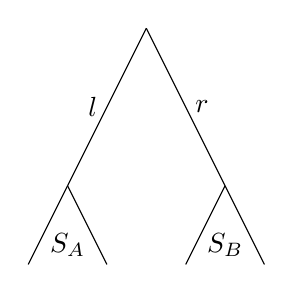
\begin{tikzpicture}
  \coordinate (P) at (0,2);
  \coordinate (A) at (-1.0,0);
  \coordinate (A1) at (-1.5,-1.0);
  \coordinate (A2) at (-0.5,-1.0);
  \coordinate (B) at (1,0);
  \coordinate (B1) at (0.50,-1.0);
  \coordinate (B2) at (1.5,-1.0);
  \node (SA) at (-1.0,-0.75) {$S_A$};
  \node (SB) at (1.0,-0.75) {$S_B$};
  \draw[] (P) -- node [left] {$l$} (A);
  \draw[] (P) -- node [right] {$r$} (B);
  \draw[] (A) -- (A1);
  \draw[] (A) -- (A2);
  \draw[] (B) -- (B1);
  \draw[] (B) -- (B2);
\end{tikzpicture}
\]

(weak coproduct diagram) %FIXME

extends to Weak Biproducts of arbitrary Set-indexed Families of Types
$\bigoplus_{i \in I} A_i$

In Process Calculus, these constructions yield \emph{Disjointly
  Guarded Sums}

Name-free, Names controlled indirectly via Types

applying general definition of Non-determinism and Semi-additivity
obtains $p + q = p \cup q$ which is the Interpretation of
Non-determinism in the Trace Model

in $\cat{ASProc}$ with Processes as Synchronization Trees Modulo Weak
Bisimulation, $p+q$ is a Non-associative version of CSP \emph{Internal
  Choice} $p \sqcap q$


\asterism


\textbf{Input/Output}

Type $X$:
\begin{align*}
  \Sigma_X &= \{\bullet\} \\
  S_X &= \Sigma_X^*
\end{align*}

Type $Y$ for an Input/Output pair Communicating with a single Client:
\begin{align*}
  \Sigma_Y &= \{inl(\bullet), inr(\bullet)\} \\
  S_Y &= a.b.S_Y + ab.S_Y
\end{align*}
where $a$, $b$, and $ab$ are abbreviations for $\{inl(\bullet)\}$,
$\{inr(\bullet)\}$, and $\{inl(\bullet),inr(\bullet)\}$, resp.
Compatible Clients are of the form $a.b.P$ where $P$ is the
Continuation Process.

\interrobang Note the above is inferred from the examples of Clients
given in \cite{abramsky-gay-nagarajan96}: $client = a.b.client$ and
$client = a.b.nil$

$cell : X \parr ... \parr X$

\fist Note unlike in $\cat{SProc}$, the Asynchronous Ports do not need
Delays ($\delta\Delta X$)


\textbf{Safety Specifications}

the above definition of $Y$ for an Input/Output pair Communicating
with a single Client has Deadlock Freedom

Example desired Safety Specification: ``Clients of a Scheduler are
Scheduled Cyclically''

$p : A$

Type $S$ with same Alphabet as $A$ but more restricted Safety
Specification

\emph{Safety Morphism} -- $s: A \rightarrow A$ such that $p : I
\rightarrow A$ Satisfies the Specification in $S$ if and only if $p =
s \circ p$

expresses stronger Specifications without ``forgetting'' what the
Interface looks like

for $s = \id_S$ (considered as a Morphism $A \rightarrow A$ because
$S_S \subseteq S_A$), $p = s \circ p \Leftrightarrow traces(p)
\subseteq S_S$

Correctness Proofs of Processes built from Subcomponents

(scheduler example)



% --------------------------------------------------------------------
\subsection{Proof Net} \label{sec:proof_net}
% --------------------------------------------------------------------

\cite{llwiki16}

Proof Nets can be seen as a Quotient of One-sided Sequent Calculus
Proofs (\S\ref{sec:sequent_calculus}) under Commutation of Rules



% --------------------------------------------------------------------
\subsection{Geometry of Synthesis} \label{sec:geometry_of_synthesis}
% --------------------------------------------------------------------

Bounded version of Geometry of Interaction



% --------------------------------------------------------------------
\subsection{Multiobject GOI}\label{sec:multiobject_goi}
% --------------------------------------------------------------------

\cite{haghverdi-scott05}

Multiplicative Linear Logic (\S\ref{sec:multiplicative_linear_logic})

Parital Trace (\S\ref{sec:partial_trace})



% --------------------------------------------------------------------
\subsection{Linear Combinatory Algebra}\label{sec:linear_combinatory_algebra}
% --------------------------------------------------------------------

2002 - Abramsky-Haghverdi-Scott - \emph{Geometry of Interaction and Linear
  Combinatory Algebras}

used for Realisers in Quantitative Type Theory
(\S\ref{sec:quantitative_type})



% ====================================================================
\section{Calculus of Capabilities}\label{sec:capabilities_calculus}
% ====================================================================

Crary-Walker-Morrisett99 \emph{Typed Memory Management in a Calculus
  of Capabilities}

Region-based Memory Management

Continuation-passing-style Language

Chargueraud-Pottier07 \emph{Functional Translation of a Calculus of
  Capabilities}

Walker-Morrisett00 \emph{Alias Types for Recursive Data Structures}

Alias Types (\S\ref{sec:alias_type})

cf. \emph{Reflective Higher-Order (RHO) Calculus} (\S\ref{sec:rho_calculus});
Namespace Logic (\S\ref{sec:namespace_logic}), Spatial-behavioral Types
(\S\ref{sec:spatial_behavioral})



% --------------------------------------------------------------------
\subsection{Capability}\label{sec:capability}
% --------------------------------------------------------------------

Shi-Xi13 -- Views (\S\ref{sec:view}) can be seen as Linear Types for
classifying Capabilities

cf. Object-Capability Model (Information Security Model), Capability-based
Security

2013 - Drossopoulou, Noble - \emph{The Need for Capability Policies}

\emph{Deniability} specifications are Open and describe Necessary Conditions for
some Effect to take place; cf. Hoare Logic specifications describing Sufficient
Conditions and are Closed

2013 - Meredith, Stay, Drossopoulou - \emph{Policy as Types} -- (Curry-Howard
Isomorphism \S\ref{sec:curry_howard}): representation of \emph{Policy} as Types
in a Spatial Behavioral Type System (\S\ref{sec:spatial_behavioral}) for
RHO-calculus (\S\ref{sec:rho_calculus}, a variant of Asynchronous Polyadic
$\pi$-calculus \S\ref{sec:polyadic_pi_calculus}); Spatial Behavioral Types
suffice as a \emph{Security Policy Language}; Namespace Logic
(\S\ref{sec:namespace_logic}) treats the Type of a Concurrent Process as an
Assertion that it belongs to a Set of Processes, all of which satisfy some
Property, and treat these Properties as \emph{Contracts} governing the Behavior
of the Process

when $\pi$-calculus is Polarized (i.e. Channels Names are indicated as being
either $+$ Input or $-$ Output), it is an Ocap (Object-capability) Language; in
RHO Calculus, the Polarization is provided by Namespaces at the Type level

a \emph{Capability}, i.e. \emph{access} to a Behavior, power or Authority, is
represented by a \emph{Channel}
